\documentclass[
  % --- Opções da classe memoir ---
  12pt,                     % Tamanho da fonte
  % openright,              % Capítulos começam em página ímpar (insere página vazia caso preciso)
  oneside,                  % Para impressão em verso e anverso. Oposto a oneside
  a4paper,                  % Tamanho do papel
  % --- opções da classe abntex2 ---
  % chapter=TITLE,          % Títulos de capítulos convertidos em letras maiúsculas
  % section=TITLE,          % Títulos de seções convertidos em letras maiúsculas
  % subsection=TITLE,       % Títulos de subseções convertidos em letras maiúsculas
  % subsubsection=TITLE,    % Títulos de subsubseções convertidos em letras maiúsculas
  % --- opções do pacote babel ---
  % english,                % Idioma adicional para hifenização
  % french,                 % Idioma adicional para hifenização
  % spanish,                % Idioma adicional para hifenização
  portuguese,
  brazil                    % O último idioma é o principal do documento
]{abntex2}

% ---
% Pacotes básicos
% ---
% \usepackage{fourier}              % Fonte Utopia (serif)
% \usepackage{libertine}            % Fonte Libertine (serif) e Biolinum (sans)
% \usepackage{XCharter}             % Fonte serifada principal do texto: BT Charter
\usepackage[sc]{mathpazo}           % Fonte serifada principal do texto: Palatino Linotype
% \linespread{1.05}                 % Palladio/Palatino needs more leading (space between lines)
\usepackage{biolinum}               % Fonte sem serifa principal
\usepackage[utf8]{inputenc}         % Codificacao do documento
\usepackage[T1]{fontenc}            % Seleção de codigos de fonte
\usepackage{lastpage}               % Usado pela Ficha catalográfica
\usepackage{indentfirst}            % Indenta o primeiro parágrafo de cada seção.
\usepackage{color}                  % Controle das cores
\usepackage{graphicx}               % Inclusão de gráficos
\usepackage{microtype}              % Para melhorias de justificação
\usepackage{amsmath}
\usepackage{nicefrac}

\newtheorem{teo}{Teorema}[chapter]
\newtheorem{exer}{Exercício}
\newtheorem{cor}{Corolário}
\newtheorem{lem}{Lema}
\newtheorem{pro}{Proposição}[chapter]
\newtheorem{exemplo}{Exemplo}[chapter]
\newtheorem{defi}{Definição}[chapter]
\newtheorem{prop}{Propriedade}[chapter]

% ---
% NOVOS COMANDOS
% ---
\newcommand{\N}{\mathbb{N}}
\newcommand{\Z}{\mathbb{Z}}
\newcommand{\R}{\mathbb{R}}
\newcommand{\Q}{\mathbb{Q}}
\newcommand{\C}{\mathbb{C}}
\newcommand{\trav}{\,---\,}
\newcommand{\mathperiod}{\;\mathrm{.}}
\newcommand{\mathcomma}{\;\mathrm{,}}


% ---
% Pacotes adicionais
% ---
\usepackage[ruled,vlined,lined,linesnumbered,algochapter,portuguese]{algorithm2e}
\usepackage{listings}
\usepackage{multicol}
\usepackage{xspace}
\newcommand{\supress}{{[}\ldots{]}\xspace}

% ---
% Pacotes de citações
% ---
% \usepackage[brazilian,hyperpageref]{backref}        % Paginas com as citações na bibl
\usepackage[num,overcite]{abntex2cite}                % Citações padrão ABNT
\citebrackets()

% ---
% CONFIGURAÇÕES DE PACOTES
% ---

% ---
% Configurações do pacote backref
% Usado sem a opção hyperpageref de backref
% \renewcommand{\backrefpagesname}{Citado na(s) página(s):~}
% Texto padrão antes do número das páginas
% \renewcommand{\backref}{}
% Define os textos da citação
% \renewcommand*{\backrefalt}[4]{
% \ifcase #1 %
%   Nenhuma citação no texto.%
% \or
%   Citado na página #2.%
% \else
%   Citado #1 vezes nas páginas #2.%
% \fi}%


% ---
% Configurações de aparência do PDF final
% ---

% Alterando o aspecto da cor azul
\definecolor{blue}{RGB}{41,5,195}

% Informações do PDF
\makeatletter
\hypersetup{
  % pagebackref=true,
  pdftitle={\@title},
  pdfauthor={\@author},
  pdfsubject={\imprimirpreambulo},
  pdfcreator={LaTeX with abnTeX2},
  % pdfkeywords={CUDA}{autovalores}{autovetores}{diagonalização},
  colorlinks=true,           % false: boxed links; true: colored links
  linkcolor=blue,            % color of internal links
  citecolor=blue,            % color of links to bibliography
  filecolor=magenta,         % color of file links
  urlcolor=blue,
  bookmarksdepth=4,
  hidelinks
}
\makeatother

% ---
% Espaçamentos entre linhas e parágrafos
% ---
% O tamanho do parágrafo é dado por:
\setlength{\parindent}{1.3cm}

% Controle do espaçamento entre um parágrafo e outro:
\setlength{\parskip}{0.2cm}  % tente também \onelineskip

% ---
% Apresentação/formatação da epígrafe dos capítulos
% ---
\epigraphfontsize{\small\itshape}
\setlength{\epigraphwidth}{0.6\textwidth}
\setlength{\epigraphrule}{0pt}

\usepackage{xifthen} % provides \isempty command below
\newcommand{\epiauthor}[2][]{%
  \ifthenelse{\isempty{#1}}%
  {\textnormal{\textsc{---#2}}}% if #1 is empty
  {\textnormal{\textsc{---#2}}, #1}% if #1 is not empty
}

\usepackage{tikz}
\usetikzlibrary{arrows.meta, positioning}
\usetikzlibrary{decorations.markings}
\usetikzlibrary{shapes.geometric,shapes.symbols,shapes.misc}
\tikzset{
  start_end/.style={
      rectangle,
      rounded corners,
      text width=3cm, draw,
      minimum height=1.3cm,
      text centered,
    },
  process/.style={
      text width=3cm, draw,
      minimum height=1.3cm,
      text centered,
    },
  decision/.style={
      diamond,
      aspect=2,
      text width=3cm, draw,
      minimum height=1.3cm,
      text centered,
    },
  description/.style={
      text centered,
      text width=5cm,
    },
  myarrow/.style={
      postaction={
          decorate, decoration={
              markings,mark=at position #1 with {\arrow{Stealth};}
            }
        }
    },
}

% ---
% Informações de dados para capa e folha de rosto
% ---
\titulo{Título}
\autor{Davi V. R. Feliciano}
\orientador{Luiz Antonio Ribeiro Junior}
% \coorientador{Nome do Coorientador}
\local{Brasília}
\data{\today}

\instituicao{
  	Universidade de Brasília\par
  	Campus Darcy Ribeiro
}

\tipotrabalho{Projeto de Trabalho de Conclusão de Curso}

\preambulo{
	Dissertação apresentada como Projeto de Trabalho de Conclusão
	de Curso para obtenção do grau de Bacharelado em Física pelo
	programa de graduação do Instituto de Física da Universidade
	de Brasília.
}

% ---
% Indice
% ---
\makeindex

\begin{document}

% Retira espaço extra obsoleto entre as frases.
\frenchspacing

% ---
% Elementos Pré Textuais
% ---

% ---
% Capa
% ---
\renewcommand{\imprimircapa}{
	\begin{capa}
		\center
		\ABNTEXchapterfont\Large Universidade de Brasília\par
		Campus Darcy Ribeiro\par
		\vspace*{1cm}
		{\ABNTEXchapterfont\Large\imprimirautor\par}
		\vspace{3.8cm}
		\ABNTEXchapterfont\bfseries\LARGE\imprimirtitulo
		\vfill
		\Large\imprimirlocal\par
		\Large{2022}
		\vspace*{1cm}
	\end{capa}
}
\imprimircapa

% ---
% Folha de rosto
% (o * indica que haverá a ficha bibliográfica)
% ---
\imprimirfolhaderosto*

% ---
% Inserir a ficha bibliográfica
% ---
% Isto é um exemplo de Ficha Catalográfica, ou ``Dados internacionais de
% catalogação-na-publicação''. Você pode utilizar este modelo como referência.
% Porém, provavelmente a biblioteca da sua universidade lhe fornecerá um PDF
% com a ficha catalográfica definitiva após a defesa do trabalho. Quando estiver
% com o documento, salve-o como PDF no diretório do seu projeto e substitua todo
% o conteúdo de implementação deste arquivo pelo comando abaixo:
%
% \begin{fichacatalografica}
%   \includepdf{ficha-catalog-disserta-wilson.pdf}
% \end{fichacatalografica}
% ---
% \begin{fichacatalografica}
  \vspace*{\fill}                   % Posição vertical
  \hrule                            % Linha horizontal
  \begin{center}                    % Minipage Centralizado
    \begin{minipage}[c]{12.5cm}     % Largura
      
      \imprimirautor
      
      \hspace{0.5cm} \imprimirtitulo  / \imprimirautor. --
      \imprimirlocal, \imprimirdata.
      
      \hspace{0.5cm} \pageref{LastPage} p.: il. (algumas color.) ; 30 cm.\\
      
      \hspace{0.5cm} \imprimirorientadorRotulo~\imprimirorientador\\
      
      \hspace{0.5cm}
      \parbox[t]{\textwidth}{\imprimirtipotrabalho~--~\imprimirinstituicao,
        \imprimirdata.}\\
      
      \hspace{0.5cm}
      1. Algoritmo Genético.
      2. Otimização Numérica.
      3. Python.
      I. Luiz Antonio Ribeiro Junior.
      II. Universidade de Brasília.
      III. Instituto de Física.
      IV. Busca por Extremos de Funções Multidimensionais Utilizando Algoritmo Genético.\\
      
      % \hspace{8.75cm} CDU 02:141:005.7\\
      
    \end{minipage}
  \end{center}
  \hrule
\end{fichacatalografica}

% ---
% Inserir folha de aprovação
% ---
% Isto é um exemplo de Folha de aprovação, elemento obrigatório da NBR
% 14724/2011 (seção 4.2.1.3). Você pode utilizar este modelo até a aprovação
% do trabalho. Após isso, substitua todo o conteúdo deste arquivo por uma
% imagem da página assinada pela banca com o comando abaixo:
% \includepdf{folha_de_aprovacao_assinada.pdf}
% ---
% \begin{folhadeaprovacao}

  \begin{center}
    {\ABNTEXchapterfont\large\imprimirautor}
    
    \vspace*{\fill}\vspace*{\fill}
    \begin{center}
      \ABNTEXchapterfont\bfseries\Large\imprimirtitulo
    \end{center}
    \vspace*{\fill}
    
    \hspace{.45\textwidth}
    \begin{minipage}{.5\textwidth}
      \imprimirpreambulo
    \end{minipage}%
    \vspace*{\fill}
  \end{center}
  
  Trabalho aprovado. \imprimirlocal, 05 de agosto de 2015:
  
  \assinatura{\textbf{\imprimirorientador} \\ Orientador}
  \assinatura{\textbf{Nome do Membro Externo} \\ Membro Externo - IF-UnB}
  \assinatura{\textbf{Nome do Membro Interno} \\ Membro Interno}
  %\assinatura{\textbf{Professor} \\ Convidado 3}
  %\assinatura{\textbf{Professor} \\ Convidado 4}
  
  \begin{center}
    \vspace*{0.5cm}
    {\large\imprimirlocal}
    \par
    {\large\imprimirdata}
    \vspace*{1cm}
  \end{center}
  
\end{folhadeaprovacao}

% ---
% Dedicatória
% ---
% \begin{dedicatoria}
% 	\vspace*{\fill}
% 	\centering
% 	\noindent
% 	\textit{\def\changemargin#1#2{\list{}{\rightmargin#2\leftmargin#1}\item[]}
\let\endchangemargin=\endlist 

\begin{changemargin}{8cm}{0cm}
  \begin{flushleft}
    \vspace*{0.75\textheight}
    
    Aos meus pais, Alessandra Feliciano e Wendell Feliciano, que não mediram esforços
    em minha educação e possibilitaram a conclusão dessa importante etapa em minha vida.
    
  \end{flushleft}
\end{changemargin}}\vspace*{\fill}
% \end{dedicatoria}

% ---
% Agradecimentos
% ---
% \begin{agradecimentos}
% 	Agradeço à minha mãe Alessandra, por ter me apoiado e me aconselhado no decorrer
de toda esta jornada, ao meu pai Wendell, quem me apresentou logo cedo à ciência
e manteve em mim a curiosidade que possibilitou a conclusão deste curso e à
minha irmã, Beatriz, a quem almejo inspirar de forma similar em sua futura
trajetória. Agradeço também à minha companheira Isabela Nogueira, uma amizade
fruto da UnB que pretendo levar para a vida, quem me auxiliou e me confortou nos
momentos difíceis no decorrer deste curso. Sou grato ainda a todos os
professores e professoras que participaram de minha formação, em especial aos
professores Arsen Melikyan, Alexandre Dias e Luiz Ribeiro, e as pessoas que me
inspiraram a explorar a área da Física, das quais posso destacar Wendel Lopes e
Matheus Horovits. Por fim, agradeço aos meus amigos Victor Rebeque, Caio
Matheus, Caio César, Aléx Cortês, Nowras Ali, Daniel Andrada, Felipe
Rodrigues, Lucas Camacho, Jonatas Nogueira, Guilherme Meyer, Ricardo Augusto,
Letícia Brotherhood que contribuíram com discussões, ideias e risadas.

% \end{agradecimentos}

% ---
% Epígrafe
% ---
% \begin{epigrafe}
% 	\vspace*{\fill}
% 	\begin{flushright}
% 		\textit{``Escreva a epígrafe aqui.\\

\textnormal{Autor (1XXX--1XXX)}


				
				
				 }
% 	\end{flushright}
% \end{epigrafe}

% ---
% Resumo
% ---
\setlength{\absparsep}{18pt} % Ajusta o espaçamento dos parágrafos do resumo
\begin{resumo}
	Nas diversas áreas do conhecimento humano é bem conhecida uma série de problemas de otimização. 
A solução desses problemas consiste em encontrar em um conjunto de configurações, um subconjunto,
ou mesmo um elemento que melhor satisfaça um ou mais vínculos previamente determinados. Uma
estratégia famosa por solucionar problemas de tal classe de forma rápida e eficiente consiste no
emprego dos algoritmos genéticos. São assim chamados devido à forte inspiração em fenômenos
da biologia evolutiva\trav como mutação, recombinação (ou \textit{crossover}) e seleção\trav
na elaboração de suas etapas de execução. Neste projeto de trabalho é proposto um algoritmo genético para
a otimização de funções reais, isto é, para a procura dos pontos nos quais a função é máxima
(ou mínima). Sua implementação é feita em Python com o uso da biblioteca NumPy. 
O algoritmo foi aplicado na otimização de algumas funções de exemplo e na busca
de uma matriz Hamiltoniana do modelo $ k \cdot p $ para o melhor ajuste das bandas de
energia de condução e de valência de alguns Dicalcogenetos de Metais de Transição\trav \ch{CrS2} e
\ch{CrSe2}\trav calculadas previamente via o método DFT. Por fim, é feita uma discussão
acerca dos resultados e da eficácia e performance do programa. 

\vspace{\onelineskip}\noindent
\textbf{Palavras-chaves}: Algoritmo Genético, Otimização Numérica, Máximos de
Funções, Mínimos de Funções, Ajuste de Curvas, Dicalcogenetos de Metais de
Transição, Python.
\end{resumo}

% ---
% Abstract
% ---
\begin{resumo}[Abstract]
	\begin{otherlanguage*}{english}
		On the diverse areas of human knowledge, there are a series of well-known optimization
problems. The solution of these problems consists in finding, in a collection of configurations,
a subset, or even an element that better satisfies one or more constraints previously determined. A
famous strategy to solve such problems in a quick and efficient fashion relies on the use of
genetic algorithms. They receive such name due to the strong inspiration in phenomena of
evolutionary biology\trav like mutation, recombination (or crossover) and selection\trav in its execution. 
In this project, a genetic algorithm is proposed for the
optimization of real functions, that is, for the search of the points in which the function is
maximum (or minimum). Its implementation is done using the Python programming language, by means of the NumPy library.
The code developed was applied in the optimization of some example functions, and a discussion
was conducted concerning the results, as well as on the efficiency and performance of the implementation.

\vspace{\onelineskip}\noindent
\textbf{Keywords}: Genetic Algorithm, Numerical Optimization, Maximum of Functions, Minimum of Functions, Python.

	\end{otherlanguage*}
\end{resumo}

% ---
% Listas (tabelas, abreviaturas e siglas, símbolos etc...)
% ---
% ---
% Lista de ilustrações
% ---
\pdfbookmark[0]{\listfigurename}{lof}
\listoffigures*
\cleardoublepage

% ---
% Lista de tabelas
% ---
% \pdfbookmark[0]{\listtablename}{lot}
% \listoftables*
% \cleardoublepage

% ---
% Lista de abreviaturas e siglas
% ---
% \begin{siglas}
%   \item[CPU] Central Processing Unit
%   \item[CUDA] Compute Unified Device Architecture
% 	\item[EISPACK] Eigensystem Package
% 	\item[GPU] Graphics Processing Unit
% 	\item[LAPACK] Linear Algebra Package
% \end{siglas}

% ---
% Lista de símbolos
% ---
% \begin{simbolos}
%   \item[$||x||_2$] norma euclidiana
% \end{simbolos}


% ---
% Sumário
% ---
\pdfbookmark[0]{\contentsname}{toc}
\tableofcontents*
\cleardoublepage


% ---
% Elementos Textuais
% ---
\textual

% ---
% Capítulos
% ---
\chapter{Introdução}\label{cap_introducao}

\section{Problemas de Otimização}

Em matemática e ciência da computação, problemas de otimização consistem naqueles em que
a solução é um elemento de um conjunto de candidatos que melhor satisfaz uma determinada
série de condições. Um exemplo clássico dessa classe é o problema da mochila 
(\textit{knapsack problem}, em inglês)\cite{knapsack_wiki}, no qual
procura-se, dentre um conjunto de itens com diversos preços e pesos, o subconjunto que
maximiza o valor total. Esse valor é calculado somando-se os preços dos itens postos na
mochila. 

Entretanto a solução deve respeitar um vínculo: o peso total dos objetos escolhidos
não deve exceder o peso máximo suportado pela mochila. Tal problema não é NP-completo, e,
ainda que seja possível encontrar a solução exata usando algoritmos de programação dinâmica,
a complexidade de tais algoritmos é $ \mathcal{O} (n w) $, onde $n$ é o número de itens e $w$ é a
capacidade da bolsa. Assim, o tempo de execução para muitos itens\trav que é o caso de interesse,
usualmente\trav pode ser mais longo do que o desejado.

Outro exemplo comum de problema de otimização é o de otimização numérica, do qual constituem
solução os pontos de máximo ou mínimo global de uma função 
$ f : \R^n \rightarrow \R $. Tomemos como exemplo simples a função
\begin{equation}
  f(x, y) = \cos(n\pi r)\exp\left(-\frac{r^2}{\sigma^2}\right) \mathcomma
  \label{eq:damped_cos}
\end{equation}
definida no domínio $ [-1, 1] \times [-1, 1] $, cujo gráfico se encontra na figura (\ref{fig:damped_cos}). 
Analiticamente é fácil determinar o ponto de máximo global em $ r = 0 $ usando métodos de cálculo
para funções de múltiplas variáveis. 

Contudo, não é sempre que pode-se dispor de tal facilidade. 
Nos casos em que a função objetivo é de maior complexidade, com domínio contido espaços de maior dimensão; 
em que a função tem evolução temporal; em que a função possui diversas descontinuidades; ou em que a função
depende de variáveis aleatórias, o problema se torna impraticável de resolver de forma analítica. 
Isto posto, como desenvolver um algoritmo para encontrar a solução?

\begin{figure}
  \centering
  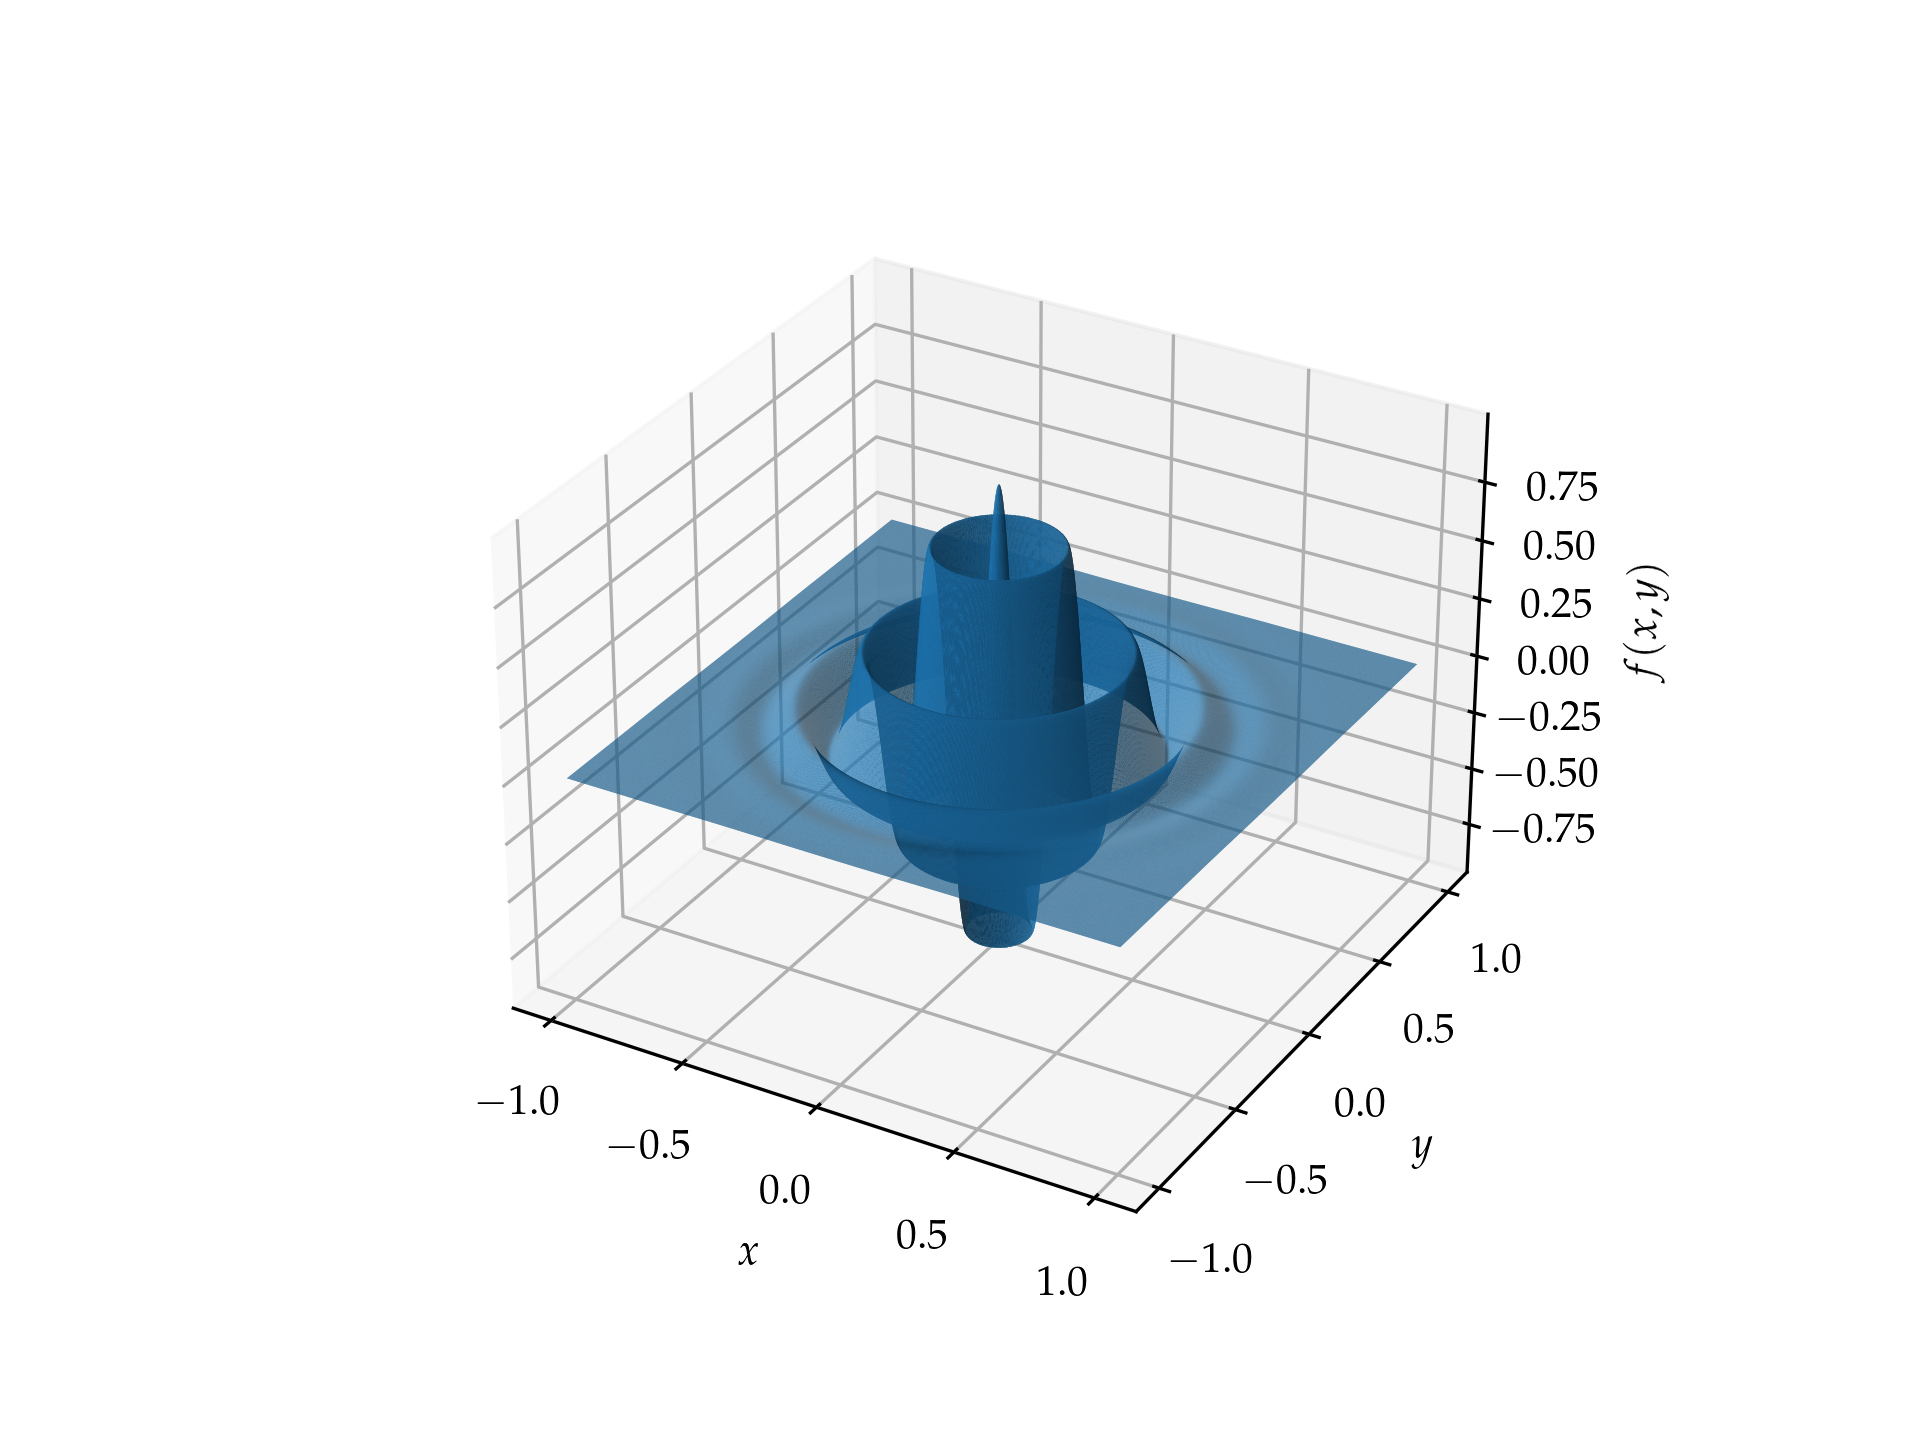
\includegraphics[width=\textwidth]{imagens/damped_cossine.png}
  \caption{Gráfico da função definida na equação (\ref{eq:damped_cos}), com $ n = 9 $ e $ \sigma = 0,4 $.}
  \label{fig:damped_cos}
\end{figure}

Uma classe de algoritmos mais simples que se propõem a resolver esse problema é são os algoritmos do
tipo \textit{hill climbing}. Sugerido pelo nome, o funcionamento desses algoritmos consiste, resumidamente,
em sortear um ponto inicial no domínio da função, calcular o gradiente da função no ponto, e seguir
na direção resultante por uma distância pré-definida, e repetir esses passos até que o módulo do
vetor gradiente seja próximo de zero, respeitando uma tolerância previamente determinada. 

O problema com esse tipo de algoritmo é que, quando aplicado em funções como a definida anteriormente, a tendência é
de que a solução encontrada seja um máximo local na grande maioria das vezes. No caso da função definida
pela equação (\ref{eq:damped_cos}), o máximo local só seria encontrado pelo algoritmo se o ponto inicial
fosse tal que $ r < \nicefrac{1}{2n} $. Se os pontos iniciais do algoritmo forem gerados aleatoriamente,
para a domínio definido, a probabilidade de um ponto pertencer a esta região é $ P(n) = \nicefrac{\pi}{16n^2} $.
Para $ n = 9 $, como na figura (\ref{fig:damped_cos}), $ P \approx 0,2\% $. 

Ademais, é possível que esse tipo
de algoritmo indique erroneamente como solução pontos de sela e planícies em determinados casos, o que o
torna ainda menos eficaz para o propósito.

Uma outra categoria de algoritmos que podem resolver ambos os problemas de forma rápida e chegar a uma
solução que se aproxima o suficiente da solução exata são os algoritmos genéticos. Tais algoritmos,
quando bem implementados podem chegar a uma solução aproximada para o problema da mochila de forma
rápida para valores de $n$ e $w$ ordens de grandeza superiores aos que tornariam praticável o uso da
estratégia proposta anteriormente. 

No problema de otimização numérica, um algoritmo desse tipo é vantajoso pois é capaz de chegar na solução
de forma rápida na maioria dos casos, identificando não só o máximo global, como também os máximos
locais contidos na região de busca. Outra vantagem é que esse método pode ser aplicado sem problemas
em espaços de busca com grande número de dimensões, ou em funções não estacionárias, contínuas ou
descontínuas. Além disso, como será mostrado posteriormente, o algoritmo é paralelizável, o que pode
acelerar a obtenção de uma solução.

\section{O Algoritmo Genético}

Os algoritmos genéticos foram primeiramente desenvolvidos por John H. 
Holland\cite{holland1992ga}\cite{holland_wiki} na década de 60. Levam esse nome pois sua formulação teve como 
forte influência o processo de evolução natural que fomenta a origem das espécies desde o surgimento da vida
em nosso planeta. Em sua execução, é inicializada uma população de indivíduos da mesma espécie\footnote{
  Isso significa que seus respectivos códigos genéticos possuem a mesma estrutura: mesma número de
  cromossomos com uma mesma quantidade de genes. Assim, pode haver reprodução entre tais indivíduos.
}.
Cada indivíduo corresponde a um candidato a solução do problema de otimização proposto, e tem sua
identidade codificada pelo seu material genético\footnote{
  No caso do problema da mochila, por exemplo, uma
  estrutura natural para o material genético é um cromossomo binário, com $n$ genes, cada um correspondente
  a um objeto do problema. Por outro lado, no problema de otimização numérica, dois cromossomos seriam
  necessários, um para codificar cada coordenada em cada dimensão do espaço de busca.
}.

Então, sob algum critério, é selecionada uma parcela desses indivíduos, a qual dará origem a novos
descendentes, cujos cromossomos serão gerados pela recombinação dos cromossomos correspondentes nos
pais. Nesse passo é introduzida uma probabilidade de mutação nos genes dos filhos. 

Ao final desse processo, descarta-se a parcela não selecionada da população, dando origem a uma nova geração, formada
pelos pais seus filhos. Esse processo é repetido iterativamente até que uma condição de parada seja
atingida. Essa condição pode ser imposta sobre o número de gerações ou sobre o tempo de execução do programa,
por exemplo.

Respeitando as diferenças de implementação em cada passo, devido as peculiaridades de cada tipo de problema
de otimização proposto, essas etapas são presentes em todo algoritmo genético, e são bem resumidas no fluxograma
presente na figura (\ref{fig:ga_flow}).

\begin{figure}
  \centering
  \begin{tikzpicture}
    \node[start_end] (start) {Início};
    \node[io, below=1em of start] (init_pop) {População\\ Inicial};
    \node[process, below=1em of init_pop]  (selection) {Seleção};
    \node[process, below=1em of selection]  (crossover) {Recombinação};
    \node[process, below=1em of crossover]  (mutation) {Mutação};
    \node[decision, below=1em of mutation]  (check) {Condição atingida?};
    \node[document, left=10ex of check] (print_stats) {Informações da\\População};
    \node[start_end, above=10ex of print_stats] (end) {Fim};
    \draw[myarrow=.9] (start.south) --  (init_pop.north);
    \draw[myarrow=.9] (init_pop.south) --  (selection.north);
    \draw[myarrow=.9] (selection.south) --  (crossover.north);
    \draw[myarrow=.9] (crossover.south) --  (mutation.north);
    \draw[myarrow=.9] (mutation.south) -- (check.north);
    \draw[myarrow=.9] (check.east) -- node[description, above] {Não} ([xshift=10ex]check.east) |- (selection.east);
    \draw[myarrow=.9] (check.west) -- node[description, above] {Sim} (print_stats.east);
    \draw[myarrow=.9] (print_stats.north) -- (end.south);
  \end{tikzpicture}
  \caption{Fluxograma geral de um algoritmo genético.}
  \label{fig:ga_flow}
\end{figure}

\newpage
\section{A Implementação}

A linguagem de programação escolhida para a implementação do algoritmo foi Python. Amplamente utilizada no meio 
acadêmico, trata-se de uma linguagem de fácil compreensão e aprendizado, além de contar com diversas bibliotecas
já implementadas com o objetivo de resolver problemas recorrentes.

As duas principais bibliotecas utilizadas neste projeto foram NumPy\cite{harris2020array} e Matplotlib\cite{hunter2007}. 
A primeira se trata de uma biblioteca para manipulação numérica e vetorizada de matrizes. É implementada na linguagem C, 
o que confere performance às operações numéricas, mantendo a facilidade de uso e versatilidade características da linguagem
Python. Já a segunda, se trata de uma biblioteca para a criação de gráficos matemáticos, que será de suma importância
na ilustração de forma clara dos resultados obtidos.

Os detalhes acerca da codificação escolhida para o material genético dos indivíduos, bem como os métodos utilizados
nas etapas de seleção, recombinação e mutação foram propostos em \citeyear{roncaratti2006ga} por \citeauthor{roncaratti2006ga},
e serão abordados de forma breve no capítulo seguinte.

\chapter{Metodologia}\label{cap_metodologia}

\section{Codificação}

\newcommand{\kth}[2]{{#1}^{(k)}_{#2}}
\newcommand{\kpth}[2]{{#1}^{(k + 1)}_{#2}}
\newcommand{\xmin}[1]{x^{(min)}_{#1}}
\newcommand{\xmax}[1]{x^{(max)}_{#1}}

Seja uma população de $n$ indivíduos representada pelo conjunto
\begin{equation}
  A = \left\{ A_1\;, \mathdots,  \;A_k\;, \mathdots, \;A_n \right\} \mathcomma
\end{equation}
onde cada indivíduo tem seu código genético representado por $m$ cromossomos
de $l$ bits, de forma que, usando uma notação matricial,
\begin{equation}
  A_k = \left[
    \begin{matrix}
      \kth{a}{11} & \cdots & \kth{a}{1m} \\
      \vdots      & \ddots & \vdots      \\
      \kth{a}{l1} & \cdots & \kth{a}{lm} \\
    \end{matrix}
    \right]
  \mathcomma
\end{equation}
onde $ \kth{a}{ij} \in \{0,1\} $, para $i$, $j$ e $k$ inteiros tais que
$ i \in \left[ 0, l \right] $, $ j \in \left[ 0, m \right] $ e $ k \in \left[ 0, n \right] $.

Para um problema de otimização numérica de uma função $ f : \mathcal{C} \subseteq \R^m \rightarrow \R $,
deve existir um mapa injetivo entre $A$ e o conjunto
\begin{equation}
  X = \left\{ X_1 \; , \mathdots,  \; X_k \; , \mathdots, \; X_n \right\} \mathcomma
\end{equation}
onde
\begin{equation}
  X_k = \left( \kth{x}{1}, \mathdots, \; \kth{x}{j}, \mathdots, \; \kth{x}{m} \right)
\end{equation}
são vetores de $ \R^n $ e representam a posição do respectivo indivíduo no espaço de busca.
Tal espaço é um subconjunto de $ \mathcal{C} $ definido pelo produto cartesiano
\begin{equation}
  \mathcal{S} = \bigtimes_{j = 1}^m \; [ \xmin{j} \; , \; \xmax{j} ] \mathcomma
\end{equation}
sendo $ \xmin{j} $ e $ \xmax{j} $, respectivamente, os valores mínimo e máximo para
a coordenada $ \kth{x}{j} $.

Como $l$ bits são capazes de representar números inteiros em $ [0, 2^l) $,
uma forma natural de mapear tal intervalo
em $ [ \xmin{j} \; , \; \xmax{j} ] $ é
\begin{equation}
  x^{(k)}_j = \xmin{j} + \frac{\xmax{j} - \xmin{j}}{2^l - 1} \sum_{i = 1}^l \kth{a}{ij} 2^{i - 1} \mathcomma
\end{equation}
cuja relação inversa é determinada por
\begin{equation}
  \sum_{i = 1}^l \kth{a}{ij} 2^{i - 1} =
  \left\lfloor \frac{(\kth{x}{j} - \xmin{j})(2^l - 1)}{\xmax{j} - \xmin{j}} \right\rfloor
  \mathperiod
\end{equation}

\section{Seleção}

Para o processo de seleção é introduzida uma nova função, denominada função desempenho.
Tal função é alguma função $ g : \R \rightarrow \R $ a partir da qual se calcula a probabilidade
de seleção do indivíduo $k$
\begin{equation}
  P_k = \frac{g(f(X_k))}{\sum_{j = 1}^n g(f(X_j))} \mathperiod
\end{equation}

Existe uma liberdade para a escolha da função desempenho, desde que se respeite a condição a
função seja sempre positiva. A ideia é que se escolha uma função desempenho que
selecione os melhores indivíduos, mas ainda mantenha uma boa variedade genética na
próxima geração. Assim, em toda geração, em média, haverá indivíduos em todo o espaço
de busca, evitando que a solução convirja de forma muito rápida\footnote{
  Retomando a função usada como exemplo no capítulo anterior, definida na Equação
  \paref{eq:damped_cos}, se escolhermos uma função de desempenho que privilegie
  de forma desproporcional pontos onde o valor da função é maior. Dependendo da
  distribuição inicial dos indivíduos, é possível que após algumas gerações,
  toda a população se concentre em $ r = \nicefrac{1}{2n} $, que é um
  máximo local.
}.

\newcommand{\fmin}{f_{min}}
\newcommand{\fmax}{f_{max}}

\begin{equation}
  a =
  \begin{cases}
    \frac{\mu (h - 1)}{\fmax - \mu} \;, & \text{se } \fmin > \frac{h\mu - \fmax}{h - 1} \\
    \frac{\mu}{\mu - \fmin}         \;, & \text{caso contrário}
  \end{cases}
  \label{eq:linear_fit_a}
\end{equation}
\begin{equation}
  b =
  \begin{cases}
    \frac{\mu (\fmax - h\mu)}{\fmax - \mu} \;, & \text{se } \fmin > \frac{h\mu - \fmax}{h - 1} \\
    - \frac{\mu\fmin}{\mu - \fmin}         \;, & \text{caso contrário}
  \end{cases}
  \label{eq:linear_fit_b}
\end{equation}

Nesse trabalho a função desempenho usada foi uma função linear $ g(x) = ax + b $
sendo $a$ e $b$ definidos pelas Equações \paref{eq:linear_fit_a} e \paref{eq:linear_fit_b},
onde
\begin{equation}
  \fmin = \min_{X_k \in X} f(X_k) \mathcomma
\end{equation}
\begin{equation}
  \fmax = \max_{X_k \in X} f(X_k) \mathcomma
\end{equation}
$h$ é um parâmetro real maior que $1$ e $\mu$ é a média do valor de $f$ sobre a população, dada por
\begin{equation}
  \mu = \sum_{k = 1}^n \frac{f(X_k)}{n} \mathperiod
\end{equation}

A seleção do indivíduos que serão recombinados para formar a geração seguinte é feita por meio
de uma roleta simples, permitindo ou não repetições. São feitos $ \nicefrac{n}{2} $ sorteios,
já que para cada par de indivíduos recombinados, dois novos serão gerados\footnote{
  Por esse motivo, $n$ deve ser um múltiplo de 4.
}.
Desse modo, a geração subsequente será constituída pelos indivíduos pais selecionados e os seus
respectivos filhos, seguindo com $n$ indivíduos.

\section{Recombinação e Mutação}

Seja o conjunto de indivíduos selecionados
\begin{equation}
  S = \left\{ S_1\;, \mathdots,  \;S_k\;, \mathdots, \;S_n \right\} \mathperiod
  \label{eq:selection}
\end{equation}
Estes indivíduos passarão, em pares adjacentes\footnote{
  O par $ (S_1, S_2) $ dá origem a dois indivíduos. O par $ (S_3, S_4) $ forma outros dois, e assim segue
  até que $ \nicefrac{n}{2} $ novos indivíduos sejam gerados.
}, pelo processo de recombinação e mutação, para dar origem a
geração seguinte da população. Esse processo é iniciado com o sorteio de duas posições em cada cromossomo,
para cada um desses pares. Essas posições são chamadas de pontos de recombinação.

Em seguida, o material genético dos indivíduos filhos será obtido pela união das partes complementares
de cada par de cromossomos dos pais e, por fim, são introduzidas mutações nos genes, com uma probabilidade predefinida.

\begin{figure}
  \centering
  \resizebox*{\textwidth}{!}{
    \begin{tikzpicture}
      \def\verticalmargin{1.3}
      \begin{scope}[local bounding box=fig1]
        \begin{scope}[start chain=1 going right,node distance=-0.15mm]
          \node [on chain=1,gene] (parent_1_left)     {0};
          \node [on chain=1,gene] (recomb_point_1_up) {0};
          \node [on chain=1,gene_filled]              {1};
          \node [on chain=1,gene_filled]              {0};
          \node [on chain=1,gene_filled]              {1};
          \node [on chain=1,gene_filled]              {1};
          \node [on chain=1,gene] (recomb_point_2_up) {0};
          \node [on chain=1,gene] (parent_1_right)    {1};
          \node [left=of parent_1_left] {$S_k$};
        \end{scope}
        \begin{scope}[start chain=1 going right,node distance=-0.15mm, shift={(0,-\verticalmargin)}]
          \node [on chain=1,gene] (mask_left)  {0};
          \node [on chain=1,gene]              {0};
          \node [on chain=1,gene]              {1};
          \node [on chain=1,gene]              {1};
          \node [on chain=1,gene]              {1};
          \node [on chain=1,gene]              {1};
          \node [on chain=1,gene]              {0};
          \node [on chain=1,gene] (mask_right) {0};
          \node [left=of mask_left] {$R$};
        \end{scope}
        \begin{scope}[start chain=1 going right,node distance=-0.15mm, shift={(0,-2*\verticalmargin)}]
          \node [on chain=1,gene_filled] (parent_2_left)       {1};
          \node [on chain=1,gene_filled] (recomb_point_1_down) {1};
          \node [on chain=1,gene]                              {1};
          \node [on chain=1,gene]                              {1};
          \node [on chain=1,gene]                              {1};
          \node [on chain=1,gene]                              {0};
          \node [on chain=1,gene_filled] (recomb_point_2_down) {1};
          \node [on chain=1,gene_filled] (parent_2_right)      {0};
          \node [left=of parent_2_left] {$S_{k + 1}$};
        \end{scope}
        \begin{scope}[start chain=1 going right,node distance=-0.15mm, shift={(0,-3*\verticalmargin)}]
          \node [on chain=1,gene_mutated] (mutation_left) {1};
          \node [on chain=1,gene]                         {0};
          \node [on chain=1,gene]                         {0};
          \node [on chain=1,gene]                         {0};
          \node [on chain=1,gene]                         {0};
          \node [on chain=1,gene]                         {0};
          \node [on chain=1,gene]                         {0};
          \node [on chain=1,gene]                         {0};
          \node [left=of mutation_left] {$M$};
        \end{scope}
        \draw ($(fig1.north west)+(0,0.85)$) rectangle ($(fig1.south east)+(0.15,-0.15)$);
        \draw [densely dotted] (recomb_point_1_up.east) -- (recomb_point_1_down.east);
        \draw [densely dotted] (recomb_point_2_up.west) -- (recomb_point_2_down.west);
        \node [description, font=\tiny, above=1.5ex of recomb_point_1_up.east] {Ponto de\\ Recombinação};
      \end{scope}
      \begin{scope}[xshift=21em, local bounding box=fig2]
        \begin{scope}[start chain=1 going right,node distance=-0.15mm]
          \node [on chain=1,gene_mutated] (mut_offspring_1_left) {1};
          \node [on chain=1,gene]                                {0};
          \node [on chain=1,gene]                                {1};
          \node [on chain=1,gene]                                {1};
          \node [on chain=1,gene]                                {1};
          \node [on chain=1,gene]                                {0};
          \node [on chain=1,gene]                                {0};
          \node [on chain=1,gene] (mut_offspring_1_right)        {1};
        \end{scope}
        \begin{scope}[start chain=1 going right,node distance=-0.15mm, shift={(0,-1*\verticalmargin)}]
          \node [on chain=1,gene] (offspring_1_left)  {0};
          \node [on chain=1,gene]                     {0};
          \node [on chain=1,gene]                     {1};
          \node [on chain=1,gene]                     {1};
          \node [on chain=1,gene]                     {1};
          \node [on chain=1,gene]                     {0};
          \node [on chain=1,gene]                     {0};
          \node [on chain=1,gene] (offspring_1_right) {1};
        \end{scope}
        \begin{scope}[start chain=1 going right,node distance=-0.15mm, shift={(0,-2*\verticalmargin)}]
          \node [on chain=1,gene_filled] (offspring_2_left)  {1};
          \node [on chain=1,gene_filled]                     {1};
          \node [on chain=1,gene_filled]                     {1};
          \node [on chain=1,gene_filled]                     {0};
          \node [on chain=1,gene_filled]                     {1};
          \node [on chain=1,gene_filled]                     {1};
          \node [on chain=1,gene_filled]                     {1};
          \node [on chain=1,gene_filled] (offspring_2_right) {0};
        \end{scope}
        \begin{scope}[start chain=1 going right,node distance=-0.15mm, shift={(0,-3*\verticalmargin)}]
          \node [on chain=1,gene_mutated] (mut_offspring_2_left) {0};
          \node [on chain=1,gene_filled]                         {1};
          \node [on chain=1,gene_filled]                         {1};
          \node [on chain=1,gene_filled]                         {0};
          \node [on chain=1,gene_filled]                         {1};
          \node [on chain=1,gene_filled]                         {1};
          \node [on chain=1,gene_filled]                         {1};
          \node [on chain=1,gene_filled] (mut_offspring_2_right) {0};
        \end{scope}
        \path [font=\tiny] (mask_right.east)++(0.15,0) edge node [above] {$(S_k \land R ) \lor (S_{k + 1} \land \lnot R)$} (offspring_1_left.west);
        \path [font=\tiny] (parent_2_right.east)++(0.15,0) edge node [below] {$(S_k \land \lnot R ) \lor (S_{k + 1} \land R)$} (offspring_2_left.west);
        \path [font=\tiny] (offspring_1_right.east) edge[bend right=90] node [left] {$\oplus M$} (mut_offspring_1_right.east);
        \path [font=\tiny] (offspring_2_right.east) edge[bend left=90] node [left] {$\oplus M$} (mut_offspring_2_right.east);
      \end{scope}
    \end{tikzpicture}
  }
  \caption{
    Diagrama ilustrando\trav em um caso com $m = 1$ e $l = 8$\trav a recombinação entre os indivíduos $S_k$ e $S_{k + 1}$
    e mutação nos filhos gerados segundo as respectivas máscaras de recombinação e mutação $R$ e $M$.
  }
  \label{fig:recomb_diagram}
\end{figure}


Matematicamente, podemos realizar esse processo para cada par da seguinte forma. Primeiramente, devemos
sortear os pontos de recombinação. Esse processo é feito por meio da geração de $m$ pares
de números naturais aleatórios distintos $ (\kth{\alpha}{j}, \kth{\beta}{j}) $ tais que
$ 0 \leq \kth{\alpha}{j} < \kth{\beta}{j} $ e $ \kth{\alpha}{j} \leq \kth{\beta}{j} < l $ onde
$ j = 0, 1, \dots, m $ e $ k = 0, 2, 4, \dots, \nicefrac{n}{2} - 2 $.

Posteriormente, é montada uma matriz $R$ denominada máscara de recombinação, definida por
\begin{equation}
  \kth{r}{ij} =
  \begin{cases}
    0 \;, & \text{se } i \leq \kth{\alpha}{j} \text{ ou } i > \kth{\beta}{j} \\
    1 \;, & \text{caso contrário}
  \end{cases}
  \mathcomma
\end{equation}
bem como uma máscara de mutação $M$, tal que
\begin{equation}
  \kth{m}{ij} =
  \begin{cases}
    1 \;, & \text{se houver mutação} \\
    0 \;, & \text{caso contrário}
  \end{cases}
  \mathperiod
\end{equation}

Finalmente, o conjunto dos indivíduos resultantes da recombinação da seleção no conjunto definido
pela Equação \paref{eq:selection} será
\begin{equation}
  S' = \left\{ S'_1\;, \mathdots,  \;S'_k\;, \mathdots, \;S'_{\nicefrac{n}{2}} \right\}
\end{equation}
tal que
\begin{subequations}
  \begin{align}
    \kth{s'}{ij}  & = (\kth{s}{ij} \land \kth{r}{ij}) \lor (\kpth{s}{ij} \land \lnot \kth{r}{ij}) \oplus \kth{m}{ij} \mathcomma \\
    \kpth{s'}{ij} & = (\kth{s}{ij} \land \lnot \kth{r}{ij}) \lor (\kpth{s}{ij} \land \kth{r}{ij}) \oplus \kth{m}{ij} \mathcomma
  \end{align}
\end{subequations}
onde $\lnot$, $\land$, $\lor$ e $\oplus$ são os operadores lógicos de negação, conjunção, disjunção e disjunção exclusiva,
respectivamente.

Ao final desse processo\trav resumido no diagrama presente na Figura \paref{fig:recomb_diagram}\trav
teremos uma nova população, sobre a qual poderemos ordenar os indivíduos segundo a função desempenho, verificar
as características dos primeiros, e, caso necessário, repetir o algoritmo desde a etapa de seleção.

\section{Estratégia Elitista}

Afim de garantir a reprodução das características dos melhores indivíduos na geração seguinte, uma
estratégia elitista pode ser tomada. Seja $\epsilon$ o melhor indivíduo\footnote{
  Aquele cuja solução correspondente $X_{\epsilon}$ satisfaz $ g(f(X_{\epsilon})) = \max_{X_k \in X} g(f(X_k)) $.
}
do conjunto $S$ definido na Equação \paref{eq:selection}. A ideia dessa abordagem é introduzir\trav
antes do processo se recombinação\trav cópias de $S_{\epsilon}$ na população\footnote{
  O conjunto dessas cópias é chamado de elite da população.
}
com o objetivo de preservar seu material genético, assim como recombina-lo com o de outros indivíduos, na esperança
de obter soluções ainda melhores para o problema.

Para isso, substituímos o conjunto $S$ por
\begin{equation}
  S =
  \left\{
  \underbrace{S_{\epsilon}\;, \mathdots,  \;S_{\epsilon}}_{e_1 \text{ cópias}}\;,\;
  \overbrace{S_{\epsilon}\;, \mathdots,  \;S_{\epsilon}}^{e_2 \text{ cópias}}\;,\;
  \underbrace{S_{e_1 + e_2 + 1}\;, \mathdots,  \;S_{\nicefrac{n}{2}}}_{\mathllap{e_3 \text{ cópias dentre os restantes}}}
  \right\}
  \mathcomma
\end{equation}
onde os primeiros $e_1 + e_2$ indivíduos foram trocados por $S_{\epsilon}$\footnote{
  Como a recombinação ocorre em pares, $e_1$ e $e_2$ devem ser pares.
}, e, dentre os indivíduos restantes,
são feitas $e_3$ substituições similares em posições aleatórias.

Ao final desse processo, prossegue-se para a etapa de recombinação, com o detalhe de que os primeiros $e_1$
indivíduos terão probabilidade de mutação $p_1 = 0$, os $e_2$ indivíduos seguintes e o restante da população
terão probabilidades de mutação não nulas $p_2$ e $p_3$.

Como consequência, $S_{\epsilon}$ será parte da população seguinte, uma vez que a recombinação entre um
indivíduo e seu clone dá origem a dois outros clones, na ausência de mutações. Ademais, cópias mutadas
também estarão presentes, bem como cruzamentos de $S_{\epsilon}$ com $e_3$ indivíduos distintos.
\chapter{Resultados}
\label{cap_resultados}

Neste capítulo são exibidos os resultados obtidos da aplicação do algoritmo
desenvolvido na otimização de algumas funções. Na seção \ref{sec_test_functions}
o algoritmo é utilizado para acusar máximos de algumas funções de $\R^2$ em $\R$
e na seção \ref{sec_resultados_tmdcs} é feito o ajuste das bandas de energia
dos TMDCs \ch{CrS2} e \ch{CrSe2} minimizando o desvio quadrático médio entre
os autovalores da hamiltoniana do modelo $ k \cdot p $ e os respectivos níveis
calculados previamente via DFT. Por fim, com os parâmetros ajustados, são ilustrados
alguns resultados físicos relevantes.

\section{Testes em Funções}
\label{sec_test_functions}

Nessa seção são exibidos os resultados de alguns testes em funções reais em $\R^2$. Em cada teste, 
8 populações com 1000 indivíduos com cromossomos de 32 bits são evoluídas por 100 gerações. O espaço de busca
considerado foi $ [-1,1] \times [-1, 1] $, onde os indivíduos foram distribuídos aleatoriamente. 
O valor usado para o parâmetro da função desempenho foi $h = 2$,
as configurações para a elite foram $e_1 = 4$, $e_2 = 6$ e $e_3 = 10$ e as probabilidades de mutação $p_2$ e $p_3$ escolhidas
foram $p_2 = 5\%$ e $p_3 = 5\%$.

Ao final do processo,
foram gerados gráficos com as curvas de nível de cada função e com as posições de todos os
integrantes de todas as populações. Os 8 melhores indivíduos são marcados de forma distinta,
afim de atestar se o algoritmo foi capaz ou não de encontrar a solução real do problema.
Um segundo gráfico com os valores das funções dos 200 melhores indivíduos de cada população
no decorrer das gerações foi gerado, a fim de mostrar, em caso de convergência, sua rapidez.

Ambos os gráficos foram feitos novamente com probabilidades de mutação $p_2 = p_3 = 20\%$
para demonstrar o papel da mutação no decorrer do algoritmo, e averiguar seu impacto na diversidade genética
dos indivíduos.
Por fim, é feita uma breve discussão sobre a performance da implementação do algoritmo e sua
complexidade de tempo de execução.

A primeira função testada foi
\begin{align}
  \begin{split}    
    f_1(x,y) & = \cos(9\pi r)\exp\left\{-\frac{r^2}{(0,4)^2}\right\} \;\text{, com} \\
    r      & = \sqrt{
      \left(x - 0,5\right)^2 +
      \left(y - 0,5\right)^2
    }
  \end{split}
  \label{eq:func_damped_cossine}
\end{align}
cujo gráfico se encontra na Figura \ref{fig:graph_damped_cossine} e os
resultados obtidos estão dispostos nas Figuras \ref{fig:contour_damped_cossine},
\ref{fig:evolution_damped_cossine}, \ref{fig:contour_damped_cossine_mut_20} e 
\ref{fig:evolution_damped_cossine_mut_20}. A segunda função testada foi
\begin{align}
  \begin{split}
    f_2(x,y) & = 0,8 \exp\left\{-\frac{r_1^2}{(0,3)^2}\right\} +
    0,88 \exp\left\{-\frac{r_2^2}{(0,03)^2}\right\} \;\text{, onde} \\
    r_1      & = \sqrt{
      \left(x - 0,5\right)^2 +
      \left(y - 0,5\right)^2
    } \;\text{ e} \\
    r_2      & = \sqrt{
      \left(x - 0,6\right)^2 +
      \left(y - 0,1\right)^2
    } \mathcomma
  \end{split}
  \label{eq:func_near_gaussians}
\end{align}
cujo gráfico se encontra na Figura \ref{fig:graph_near_gaussians} com os
resultados obtidos ilustrados nas Figuras \ref{fig:contour_near_gaussians},
\ref{fig:evolution_near_gaussians}, \ref{fig:contour_near_gaussians_mut_20} e 
\ref{fig:evolution_near_gaussians_mut_20}.

Como pode ser observado, em todos os casos, os melhores indivíduos foram localizados 
com precisão no máximo global. Não obstante, uma variedade genética proporcional a
probabilidade de mutação foi mantida, dada uma escolha correta de $p_2$ e $p_3$ para cada
problema. Nos casos em que $p_2 = 20\%$, os indivíduos, ao final do processo, se encontravam
espalhados por todo o espaço de busca. 

Vale ressaltar porém que o valor necessário de $p_2$ e $p_3$ para que uma população 
tenha a distribuição desejada depende da função a ser otimizada, como pode ser visto
comparando as Figuras \ref{fig:contour_damped_cossine_mut_20} e \ref{fig:evolution_damped_cossine_mut_20}
com as Figuras \ref{fig:contour_near_gaussians_mut_20} e \ref{fig:evolution_near_gaussians_mut_20}.
Assim, a influência dos parâmetros $p_2$, $p_3$, $e_1$, $e_2$ e $e_3$ no comportamento da população
deve ser estudada em cada caso, afim de extrair do algoritmo o resultado desejado.

Outra vantagem do algoritmo é que os máximos locais também puderam ser encontrados.
Isso pode ser observado especialmente na Figura \ref{fig:evolution_damped_cossine_mut_20},
onde visivelmente há uma concentração de indivíduos em $ f_1(x,y) \approx 0,74 $ e 
$ f_1(x,y) \approx 0,29 $, que correspondem aos dois primeiros máximos locais.
Algo similar pode ser observado na segunda função, nas primeiras gerações da Figura 
\ref{fig:evolution_near_gaussians_mut_20}, com alguma concentração da população em
vermelho em $f_1(x,y) \approx 0,8$.

Claro que, mesmo nos casos em que não é possível inferir o máximo local da evolução
de uma parcela da população\trav como ocorre na Figura \ref{fig:evolution_damped_cossine}\trav
uma análise estatística feita sobre os valores das funções desempenho dos indivíduos e
suas respectivas posições ainda seria capaz de acusá-lo.

Em alguns casos, 100 gerações não são o suficiente para determinar a solução correta. Na população
em vermelho na Figura \ref{fig:evolution_near_gaussians} houve uma convergência rápida para o
máximo local, onde todos os 200 melhores indivíduos permaneceram durante toda a duração do teste.
Algo similar ocorreu na população em verde, para a maioria dos indivíduos da elite. Entretanto, 
o número de gerações sempre pode ser escolhido conforme a necessidade.

\begin{figure}
  \begin{subfigure}{\textwidth}
    \centering
    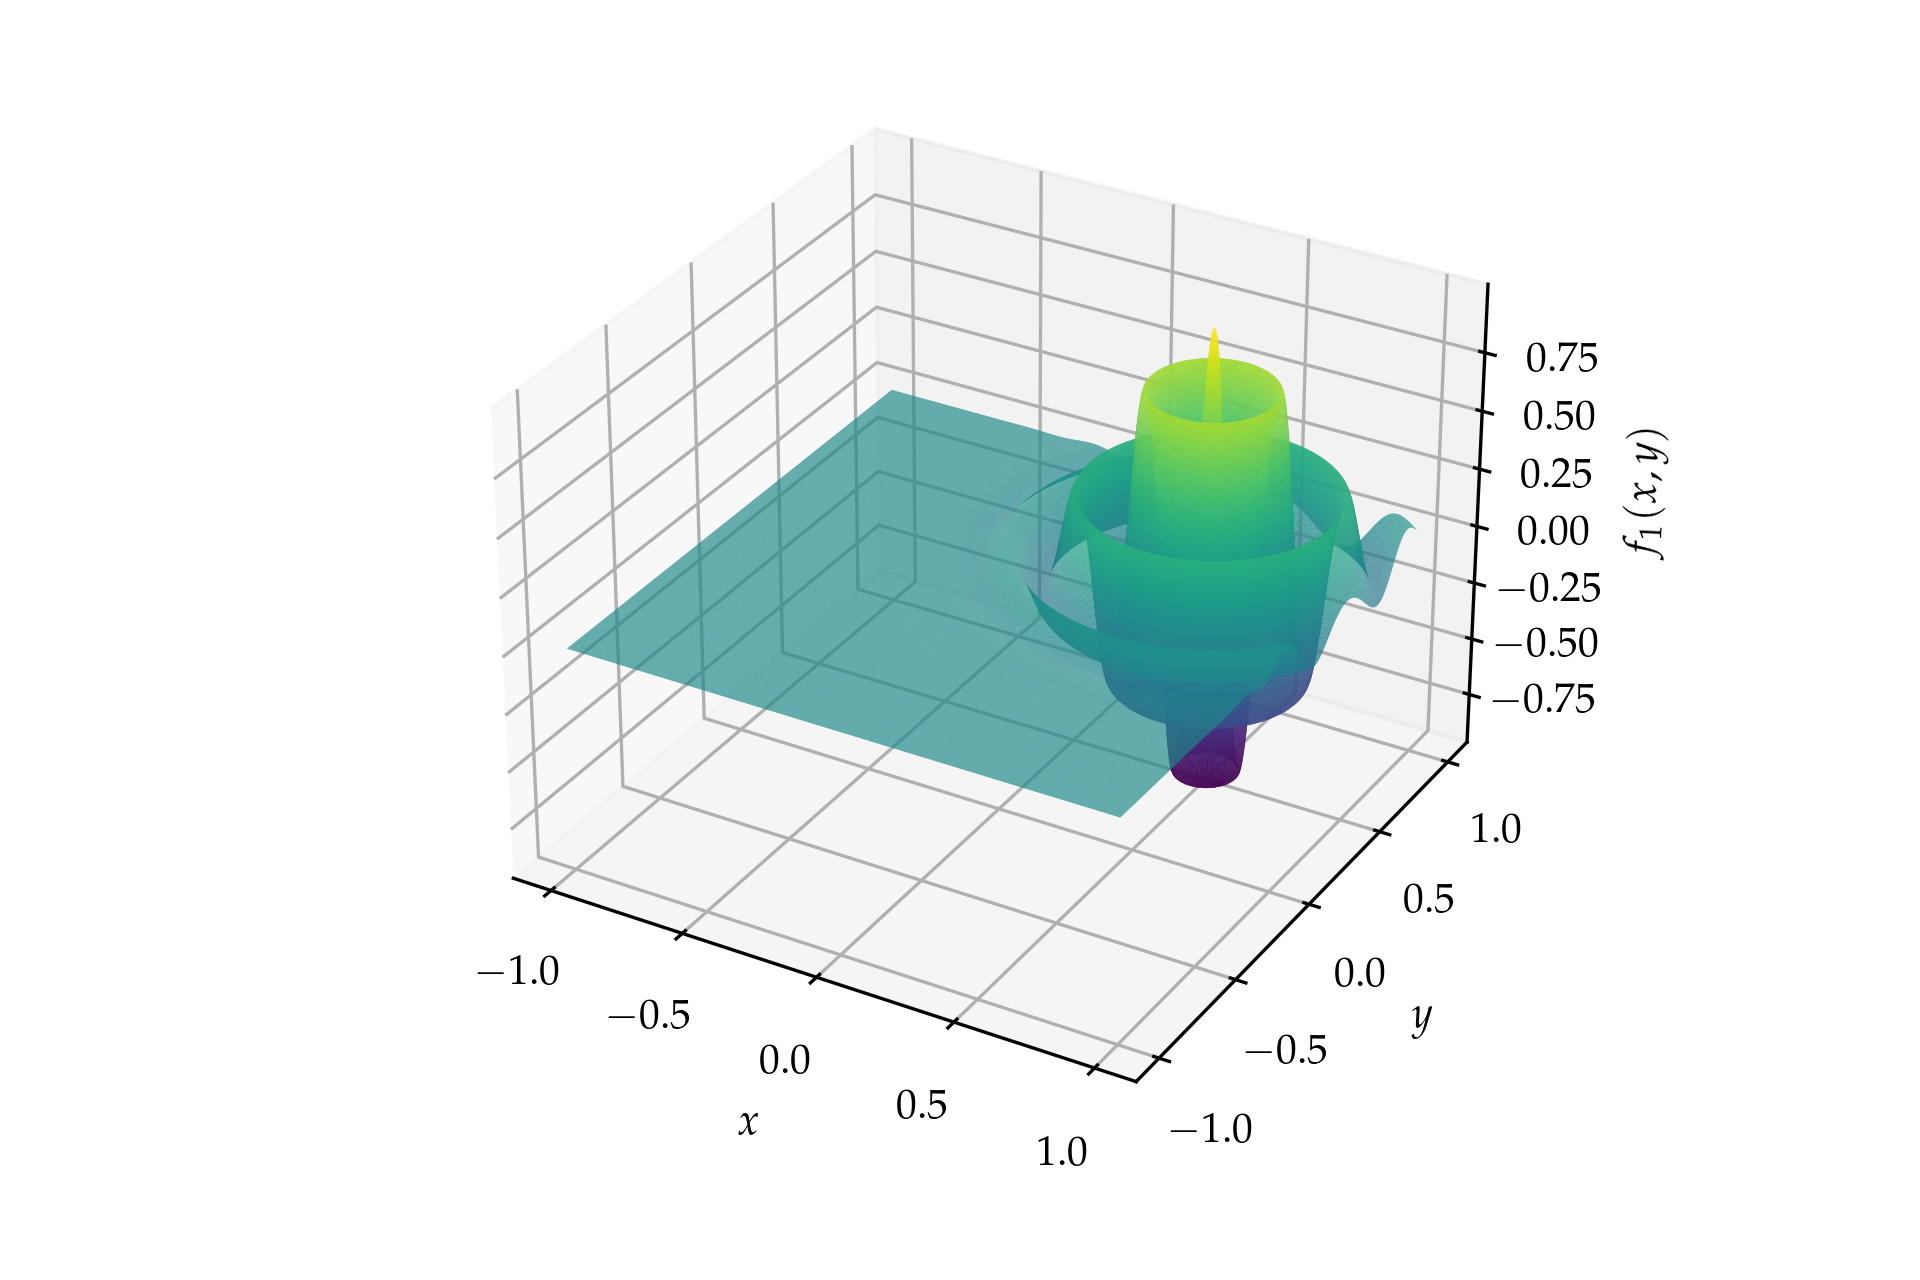
\includegraphics[width=\textwidth]{imagens/graph_damped_cossine.png}
    \caption{}
    \label{fig:graph_damped_cossine}
  \end{subfigure}
  \begin{subfigure}{\textwidth}
    \centering
    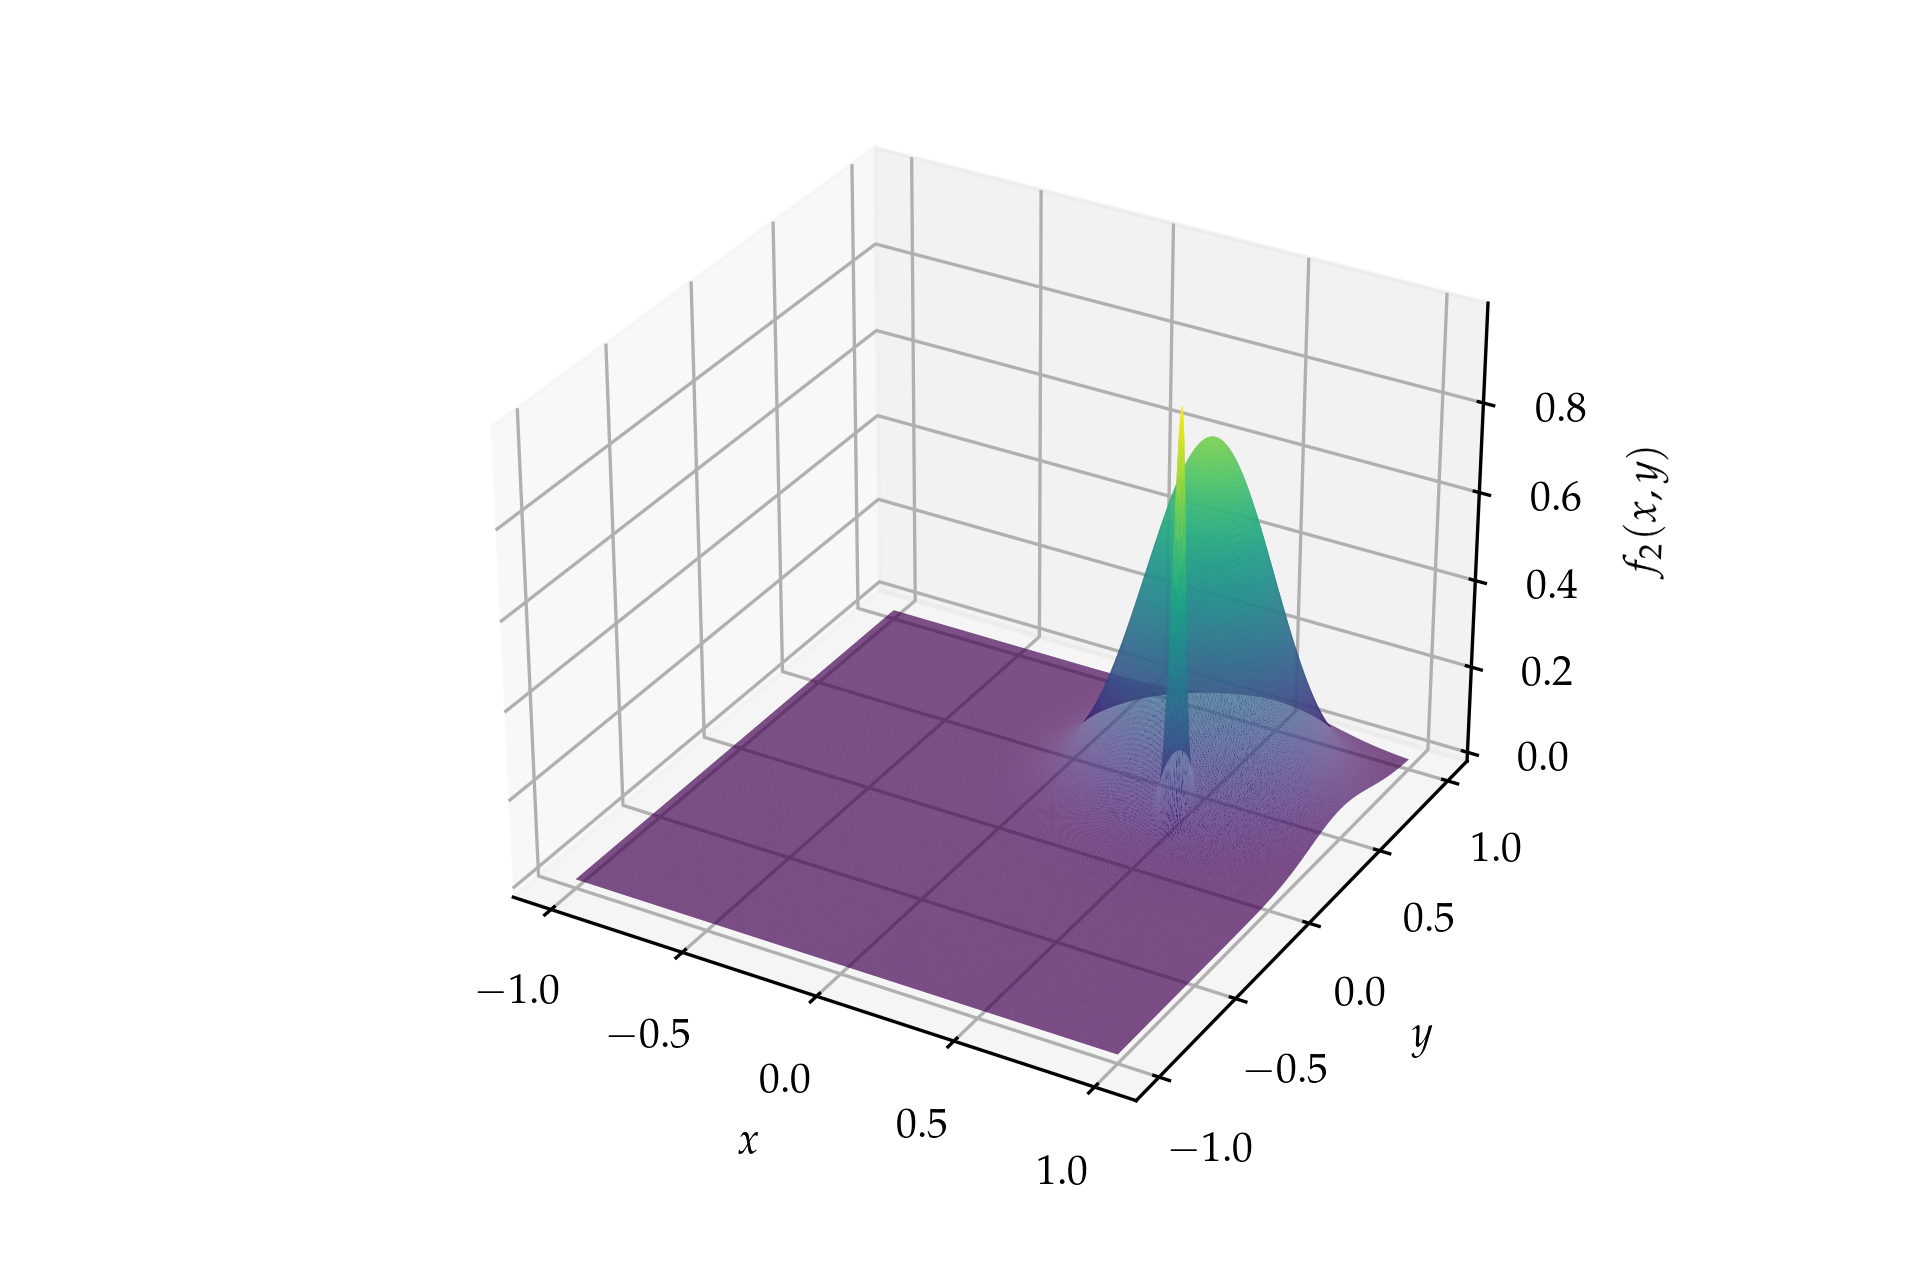
\includegraphics[width=\textwidth]{imagens/graph_near_gaussians.png}
    \caption{}
    \label{fig:graph_near_gaussians}
  \end{subfigure}
  \caption{
    \subref{fig:graph_damped_cossine} Gráfico da função $f_1(x,y)$.
    \subref{fig:graph_near_gaussians} Gráfico da função $f_2(x,y)$.
  }
\end{figure}

\begin{figure}[p]
  \centering
  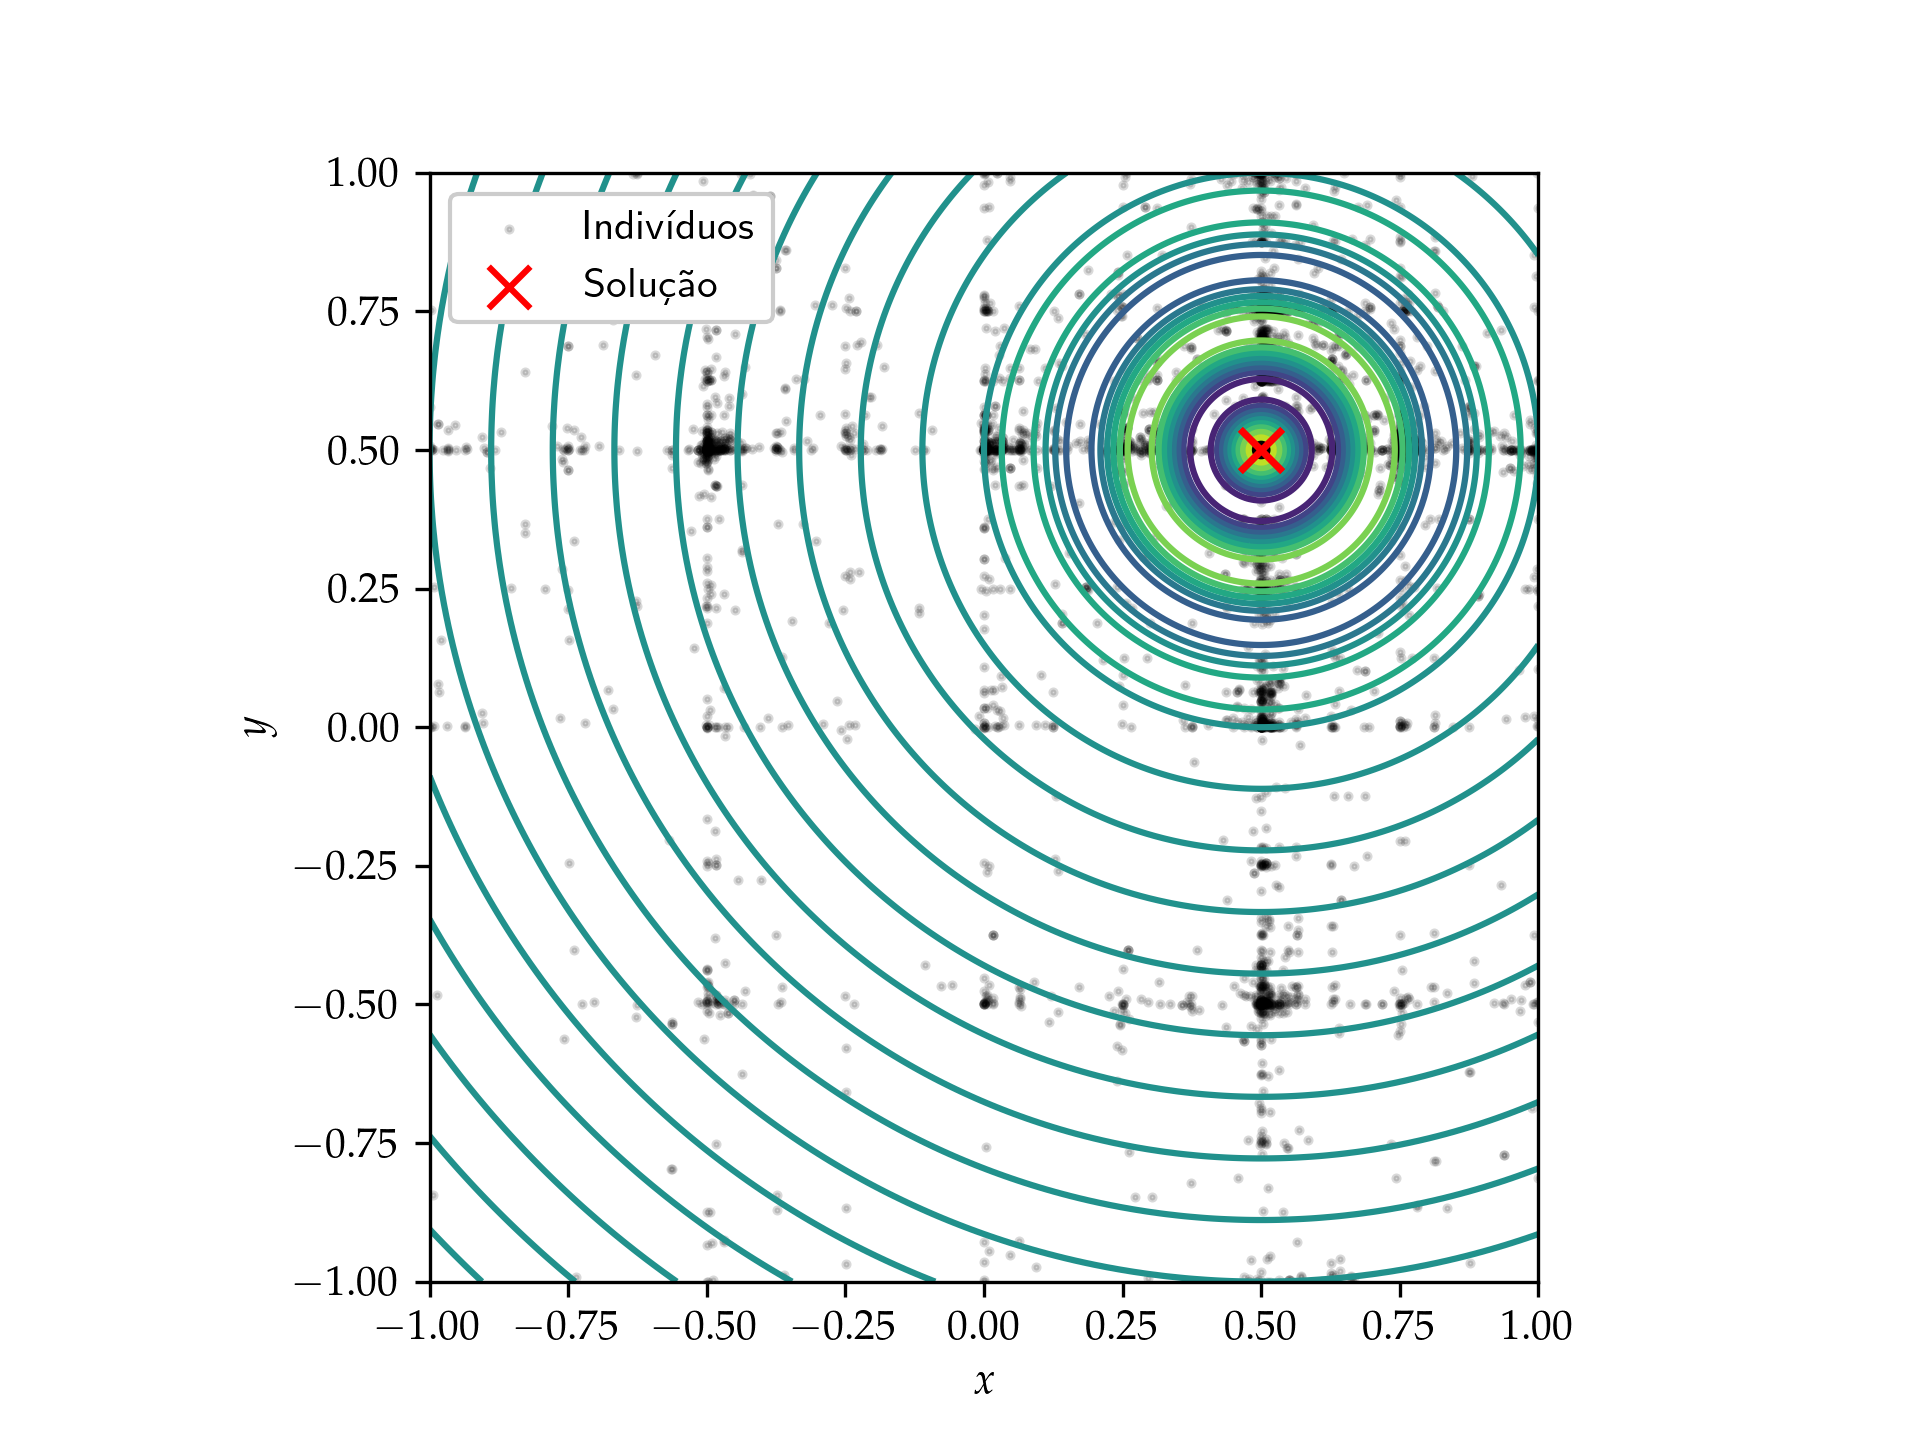
\includegraphics[width=\textwidth]{imagens/low_prob/contour_damped_cossine.png}
  \caption{
    Curvas de nível da função $f_1(x,y)$. Os pontos em preto indicam as posições dos indivíduos
    de 8 populações em sua 100ª geração na otimização da função, com $ p_2 = p_3 = 5\% $. 
    Marcado com um $\times$ vermelho estão os melhores indivíduos de cada população.
  }
  \label{fig:contour_damped_cossine}
\end{figure}

\begin{figure}[p]
  \centering
  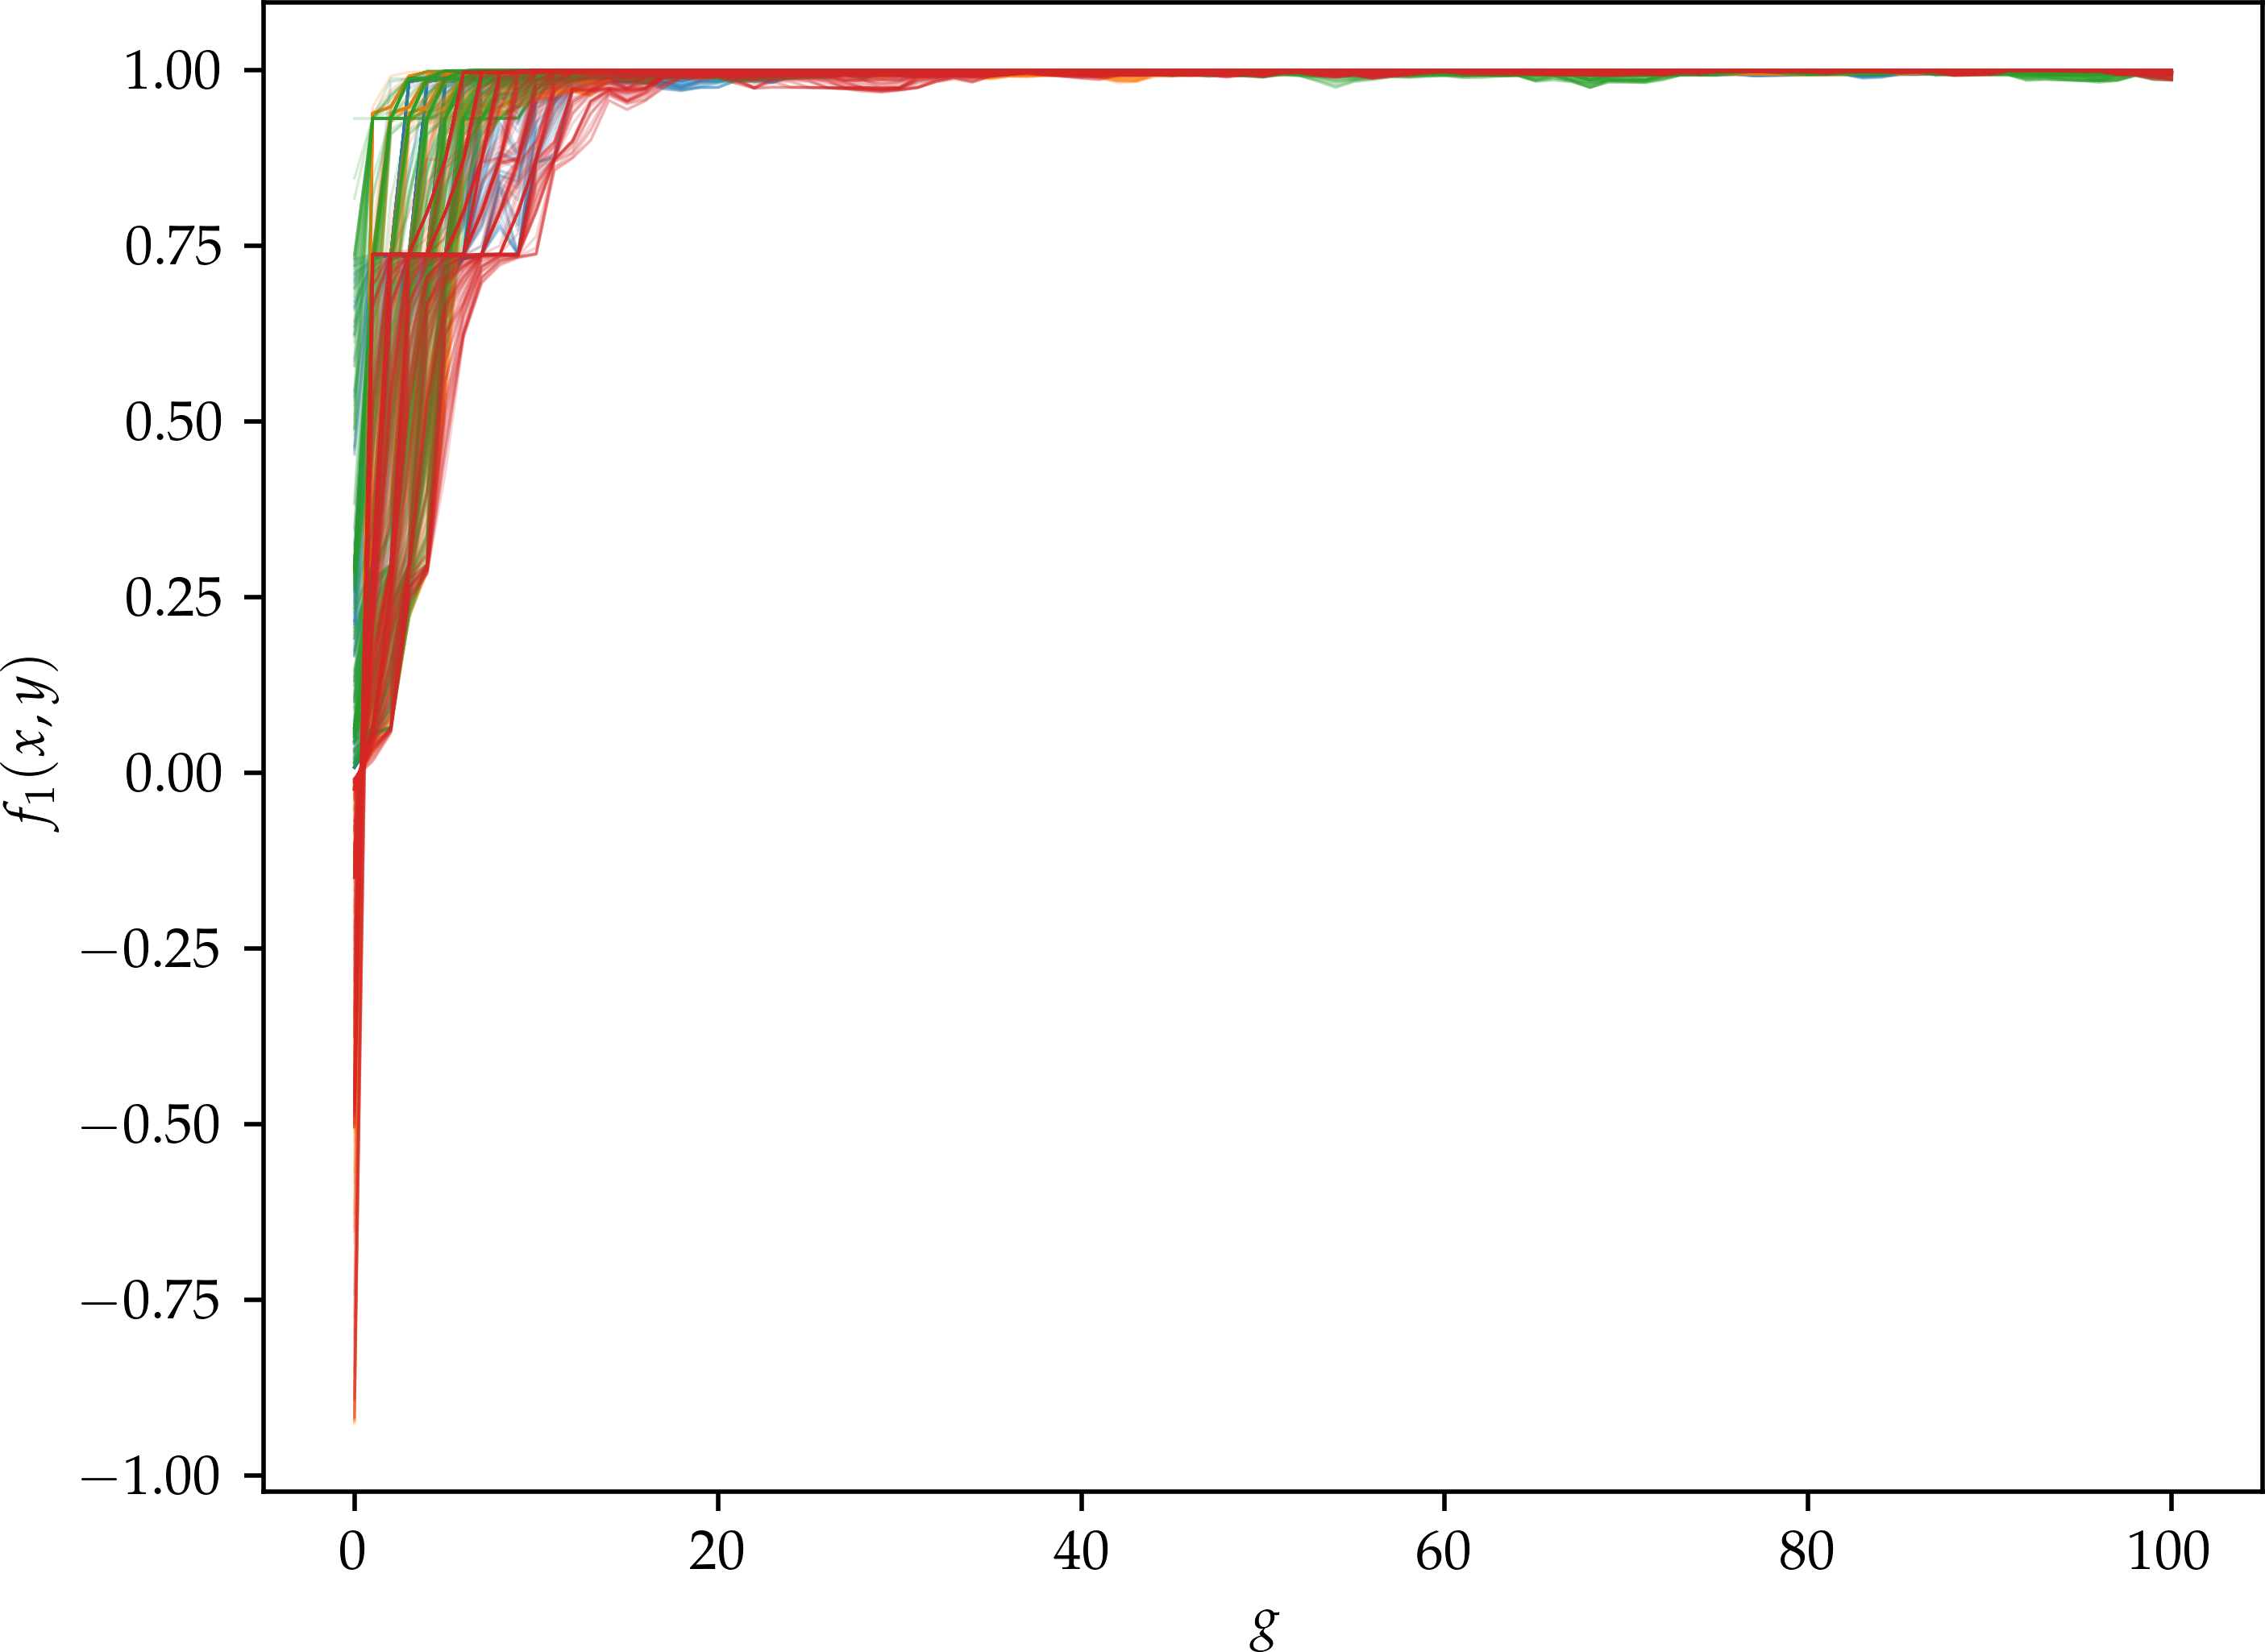
\includegraphics[width=\textwidth]{imagens/low_prob/evolution_damped_cossine.png}
  \caption{
    Evolução dos valores da função $ f_1(x,y) $ para os
    melhores 200 indivíduos de cada população, diferenciadas por cor, em termos da geração $g$,
    com $ p_2 = p_3 = 5\% $.
  }
  \label{fig:evolution_damped_cossine}
\end{figure}

\begin{figure}[p]
  \centering
  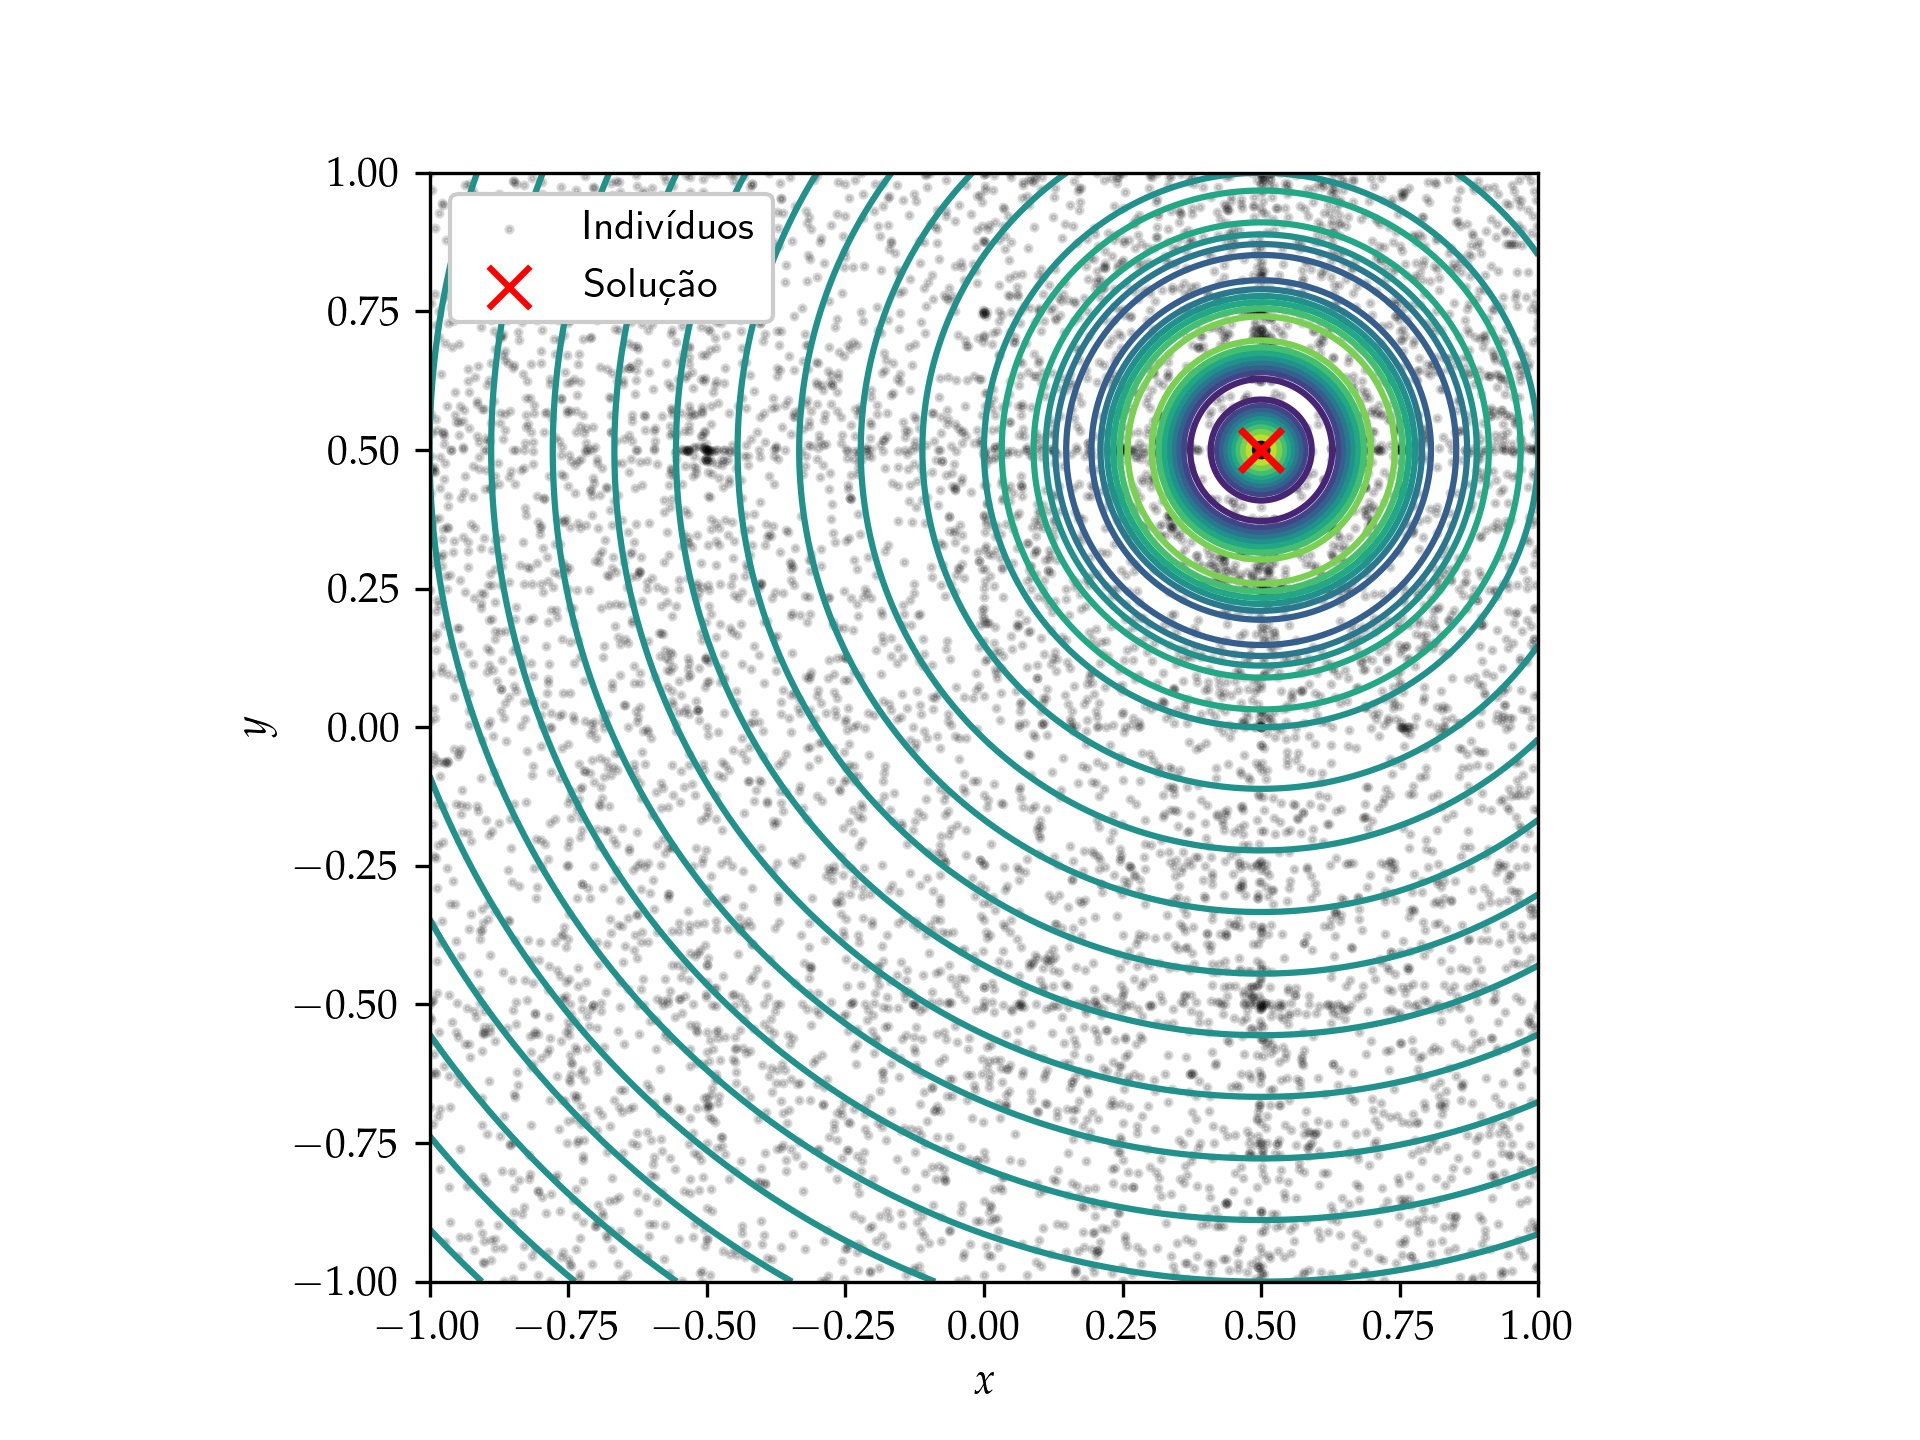
\includegraphics[width=\textwidth]{imagens/high_prob/contour_damped_cossine.png}
  \caption{
    Curvas de nível da função $f_1(x,y)$. Os pontos em preto indicam as posições dos indivíduos
    de 8 populações em sua 100ª geração na otimização da função, com $ p_2 = p_3 = 20\% $. 
    Marcado com um $\times$ vermelho estão os melhores indivíduos de cada população.
  }
  \label{fig:contour_damped_cossine_mut_20}
\end{figure}

\begin{figure}[p]
  \centering
  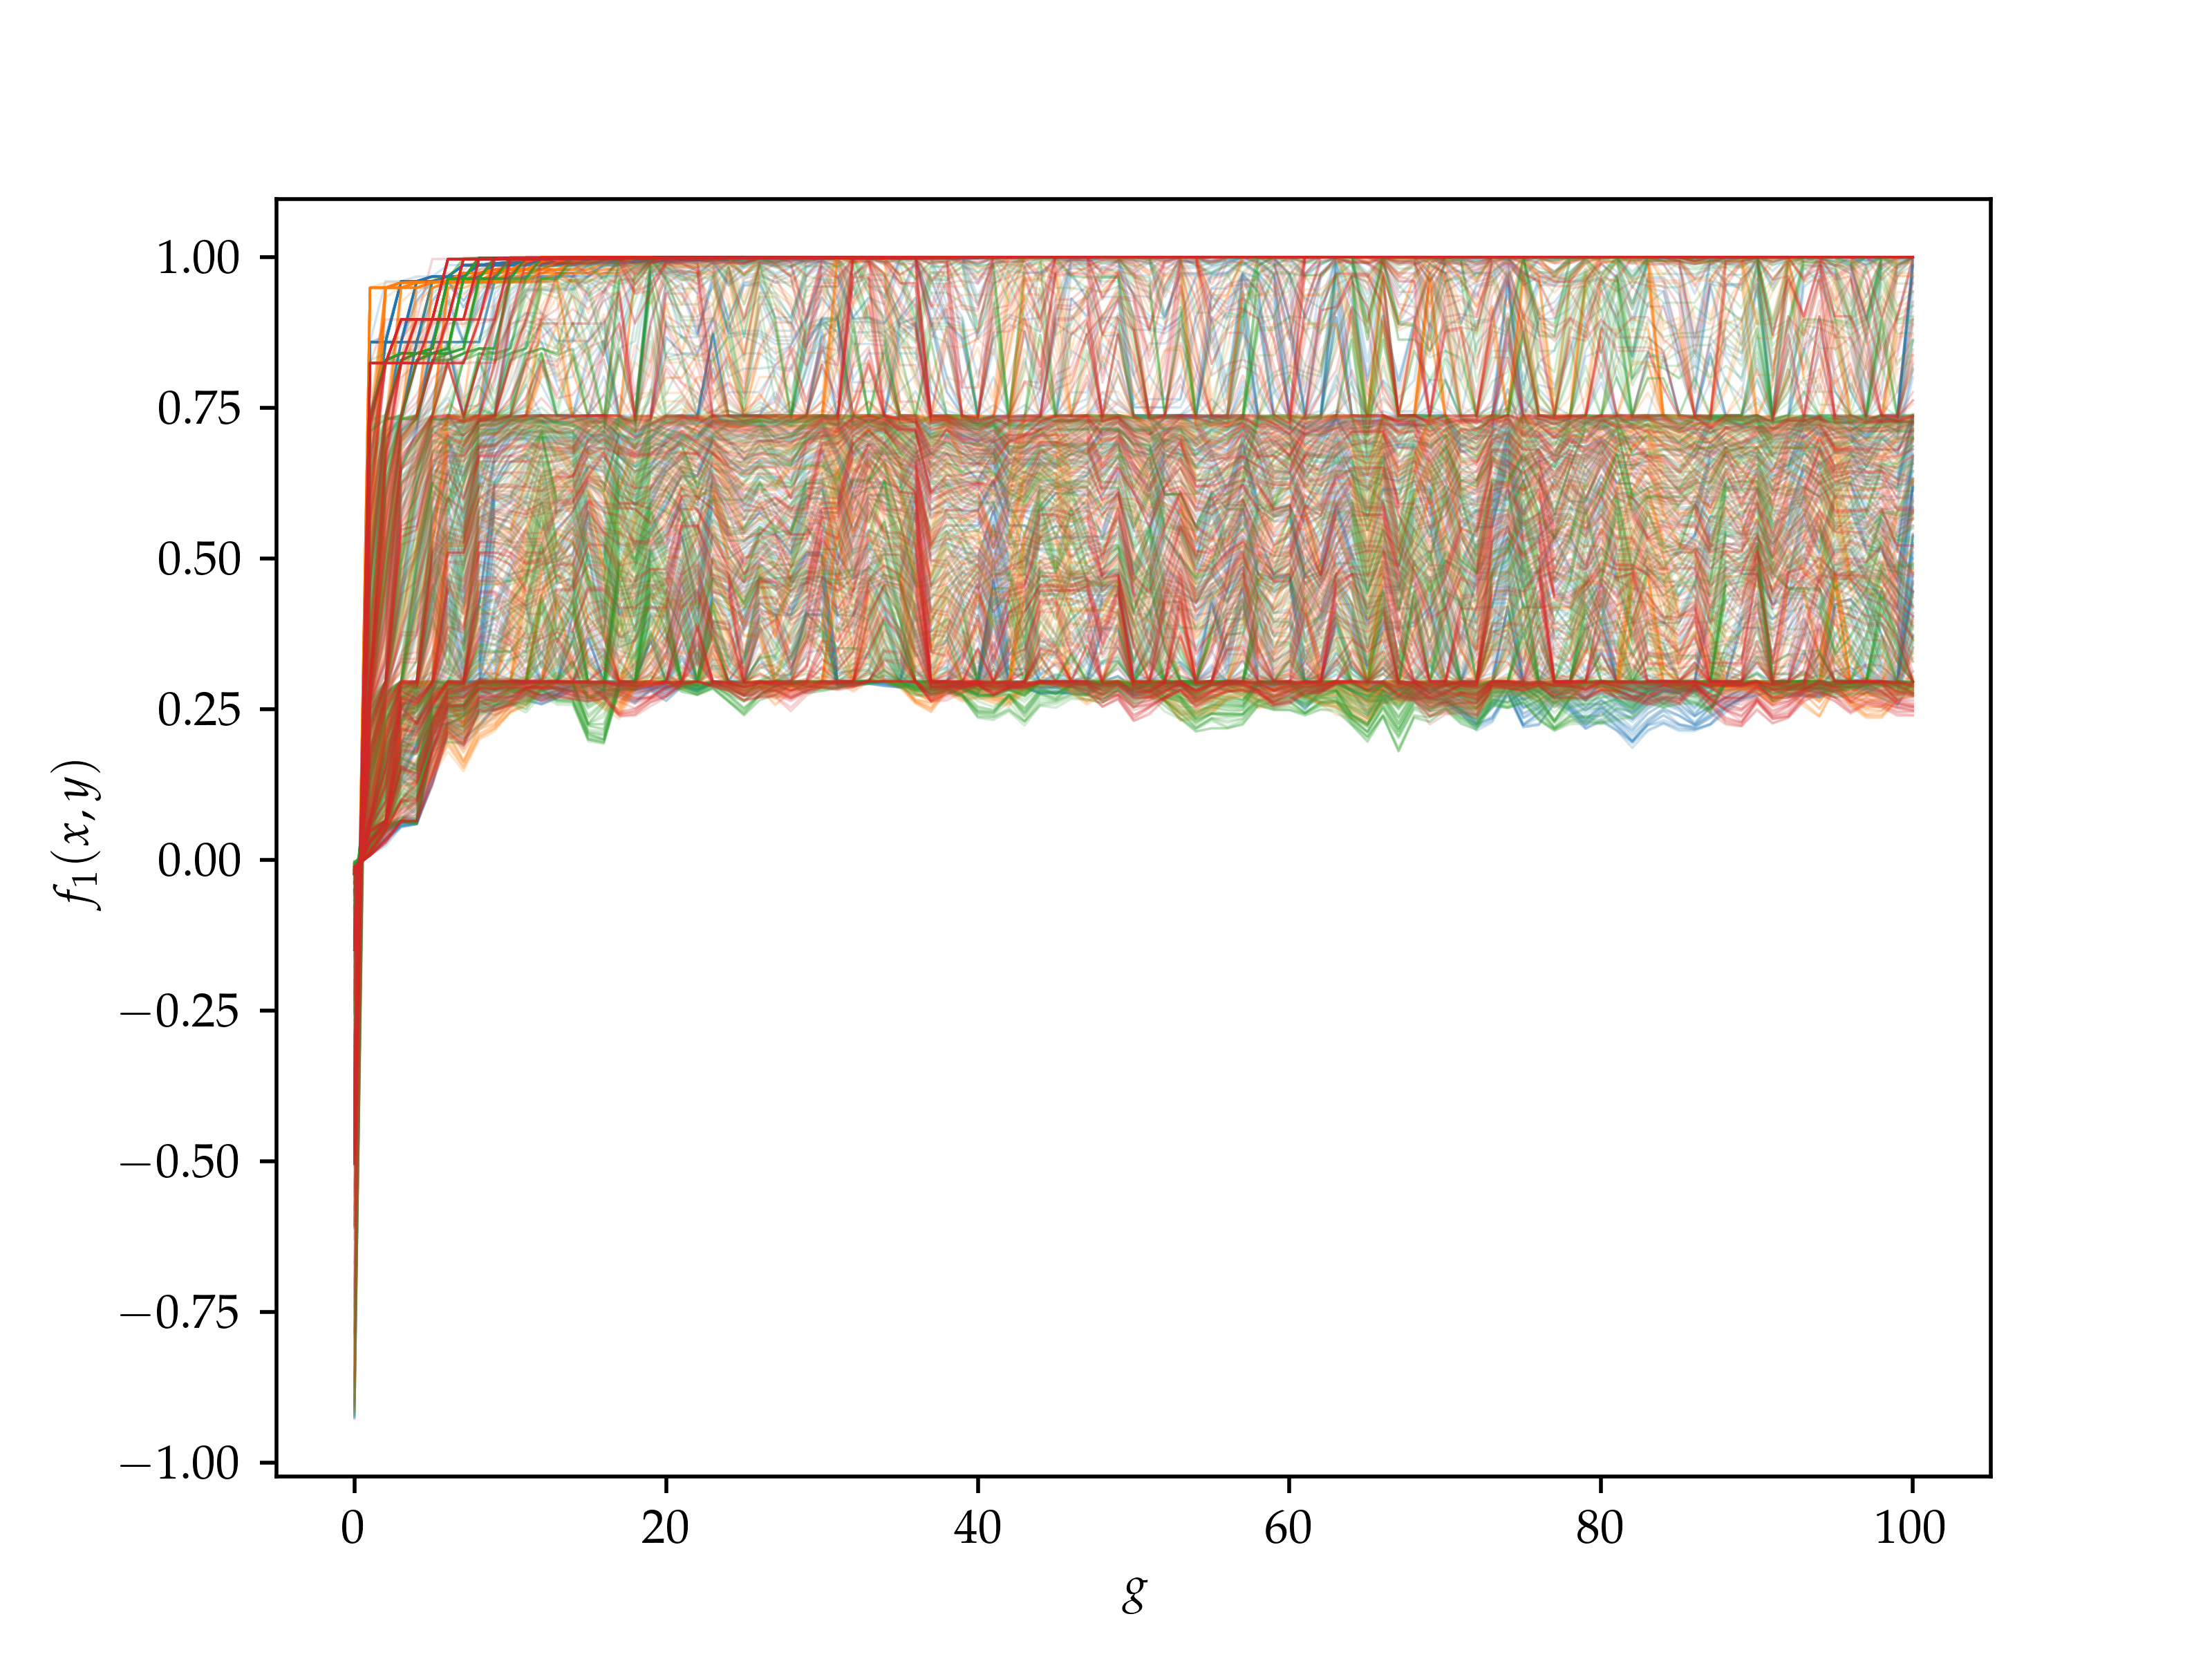
\includegraphics[width=\textwidth]{imagens/high_prob/evolution_damped_cossine.png}
  \caption{
    Evolução dos valores da função $ f_1(x,y) $ para os
    melhores 200 indivíduos de cada população, diferenciadas por cor, em termos da geração $g$,
    com $ p_2 = p_3 = 20\% $.
  }
  \label{fig:evolution_damped_cossine_mut_20}
\end{figure}

\begin{figure}[p]
  \centering
  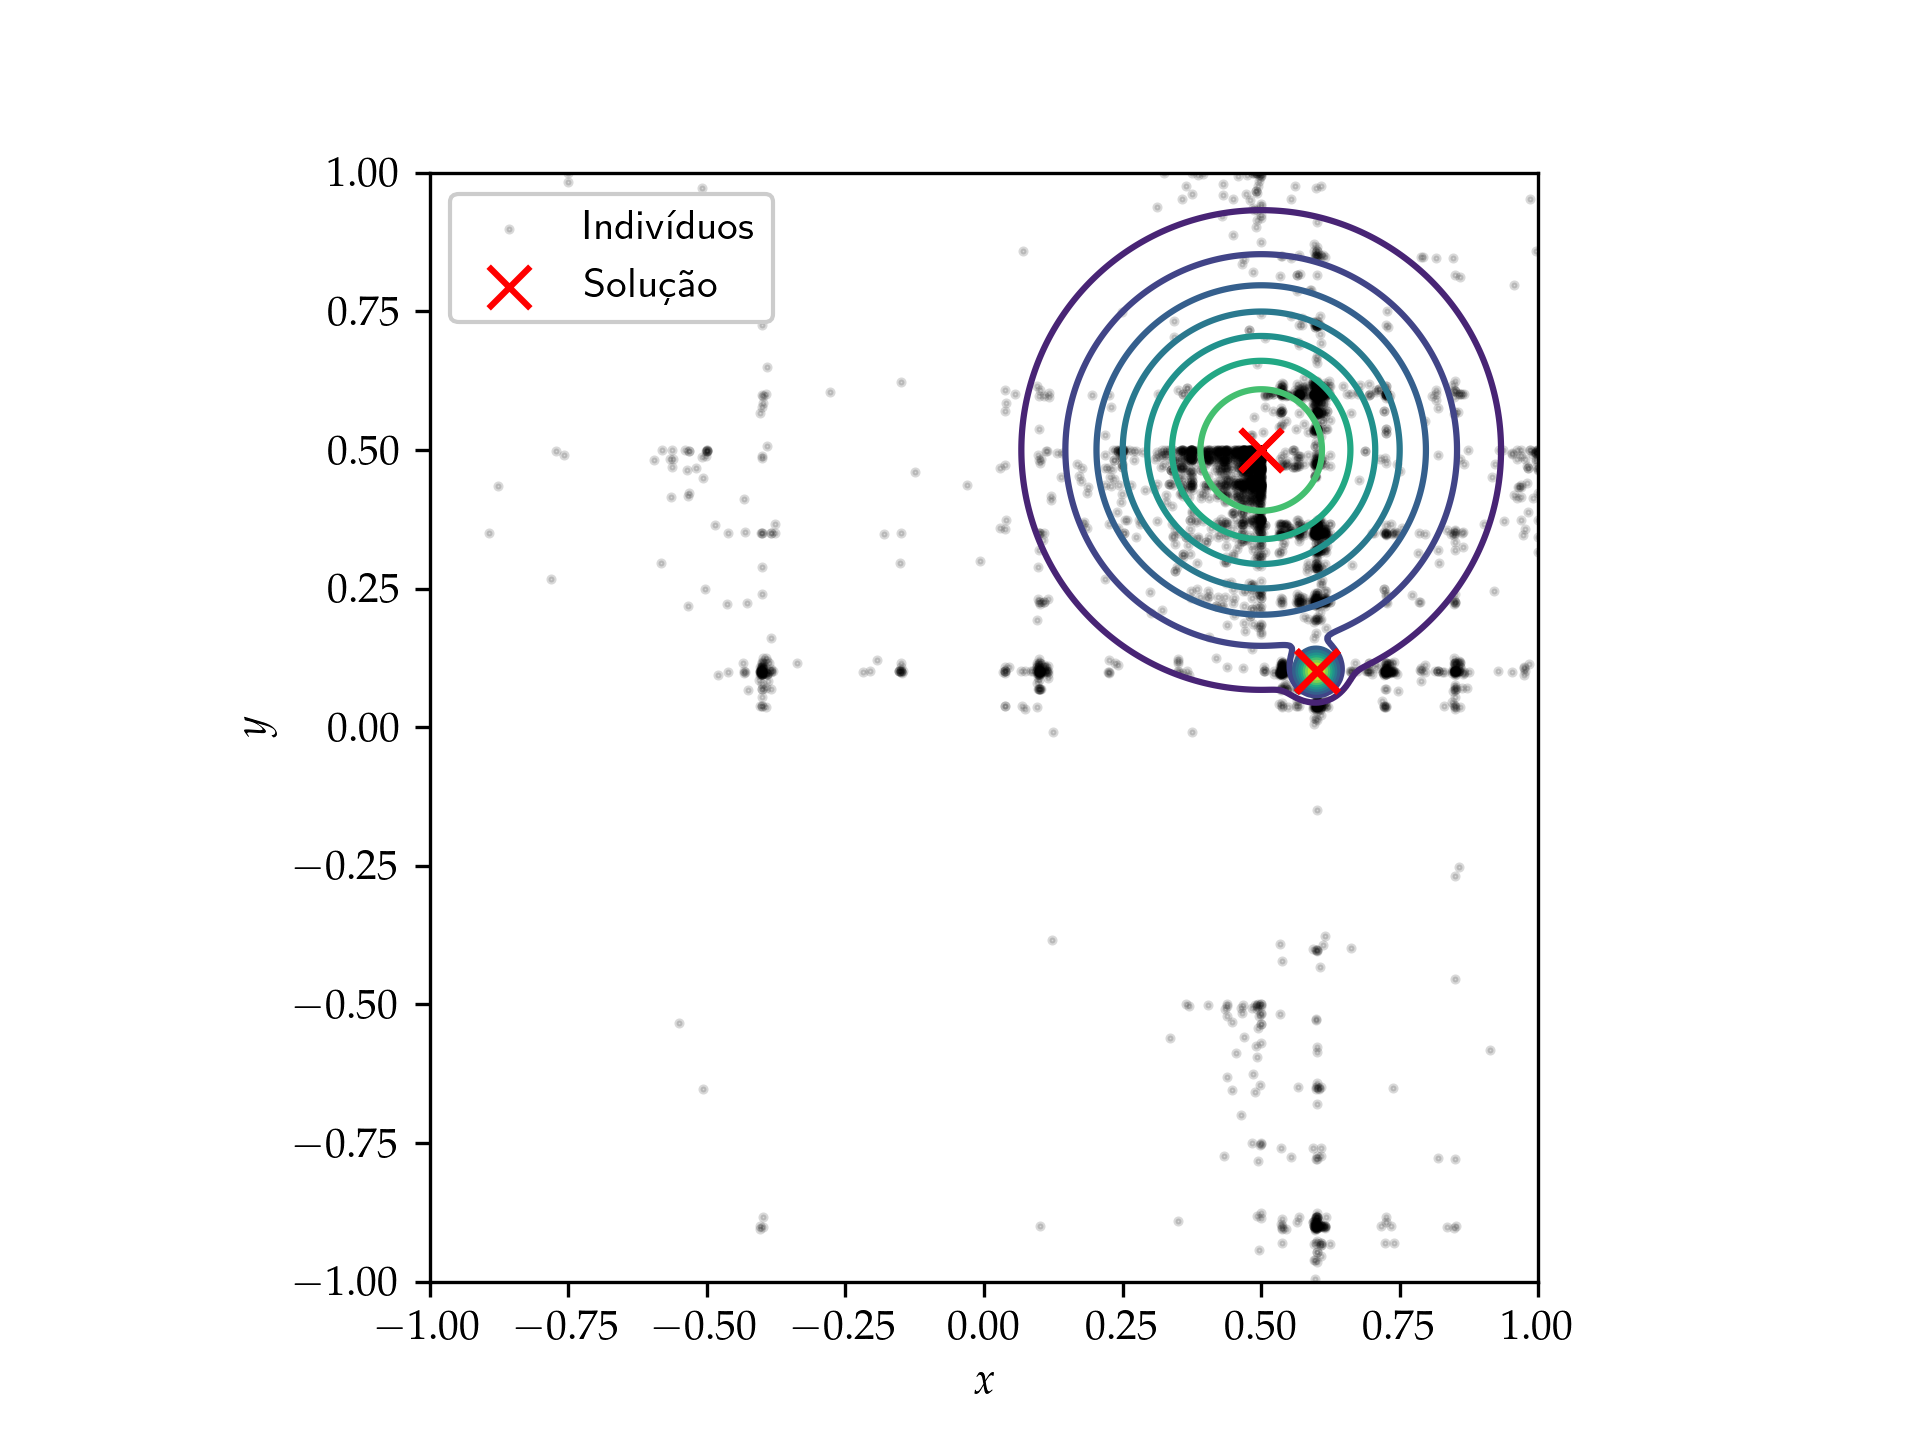
\includegraphics[width=\textwidth]{imagens/low_prob/contour_near_gaussians.png}
  \caption{
    Curvas de nível da função $f_2(x,y)$. Os pontos em preto indicam as posições dos indivíduos
    de 8 populações em sua 100ª geração na otimização da função, com $ p_2 = p_3 = 5\% $. 
    Marcado com um $\times$ vermelho estão os melhores indivíduos de cada população.
  }
  \label{fig:contour_near_gaussians}
\end{figure}

\begin{figure}[p]
  \centering
  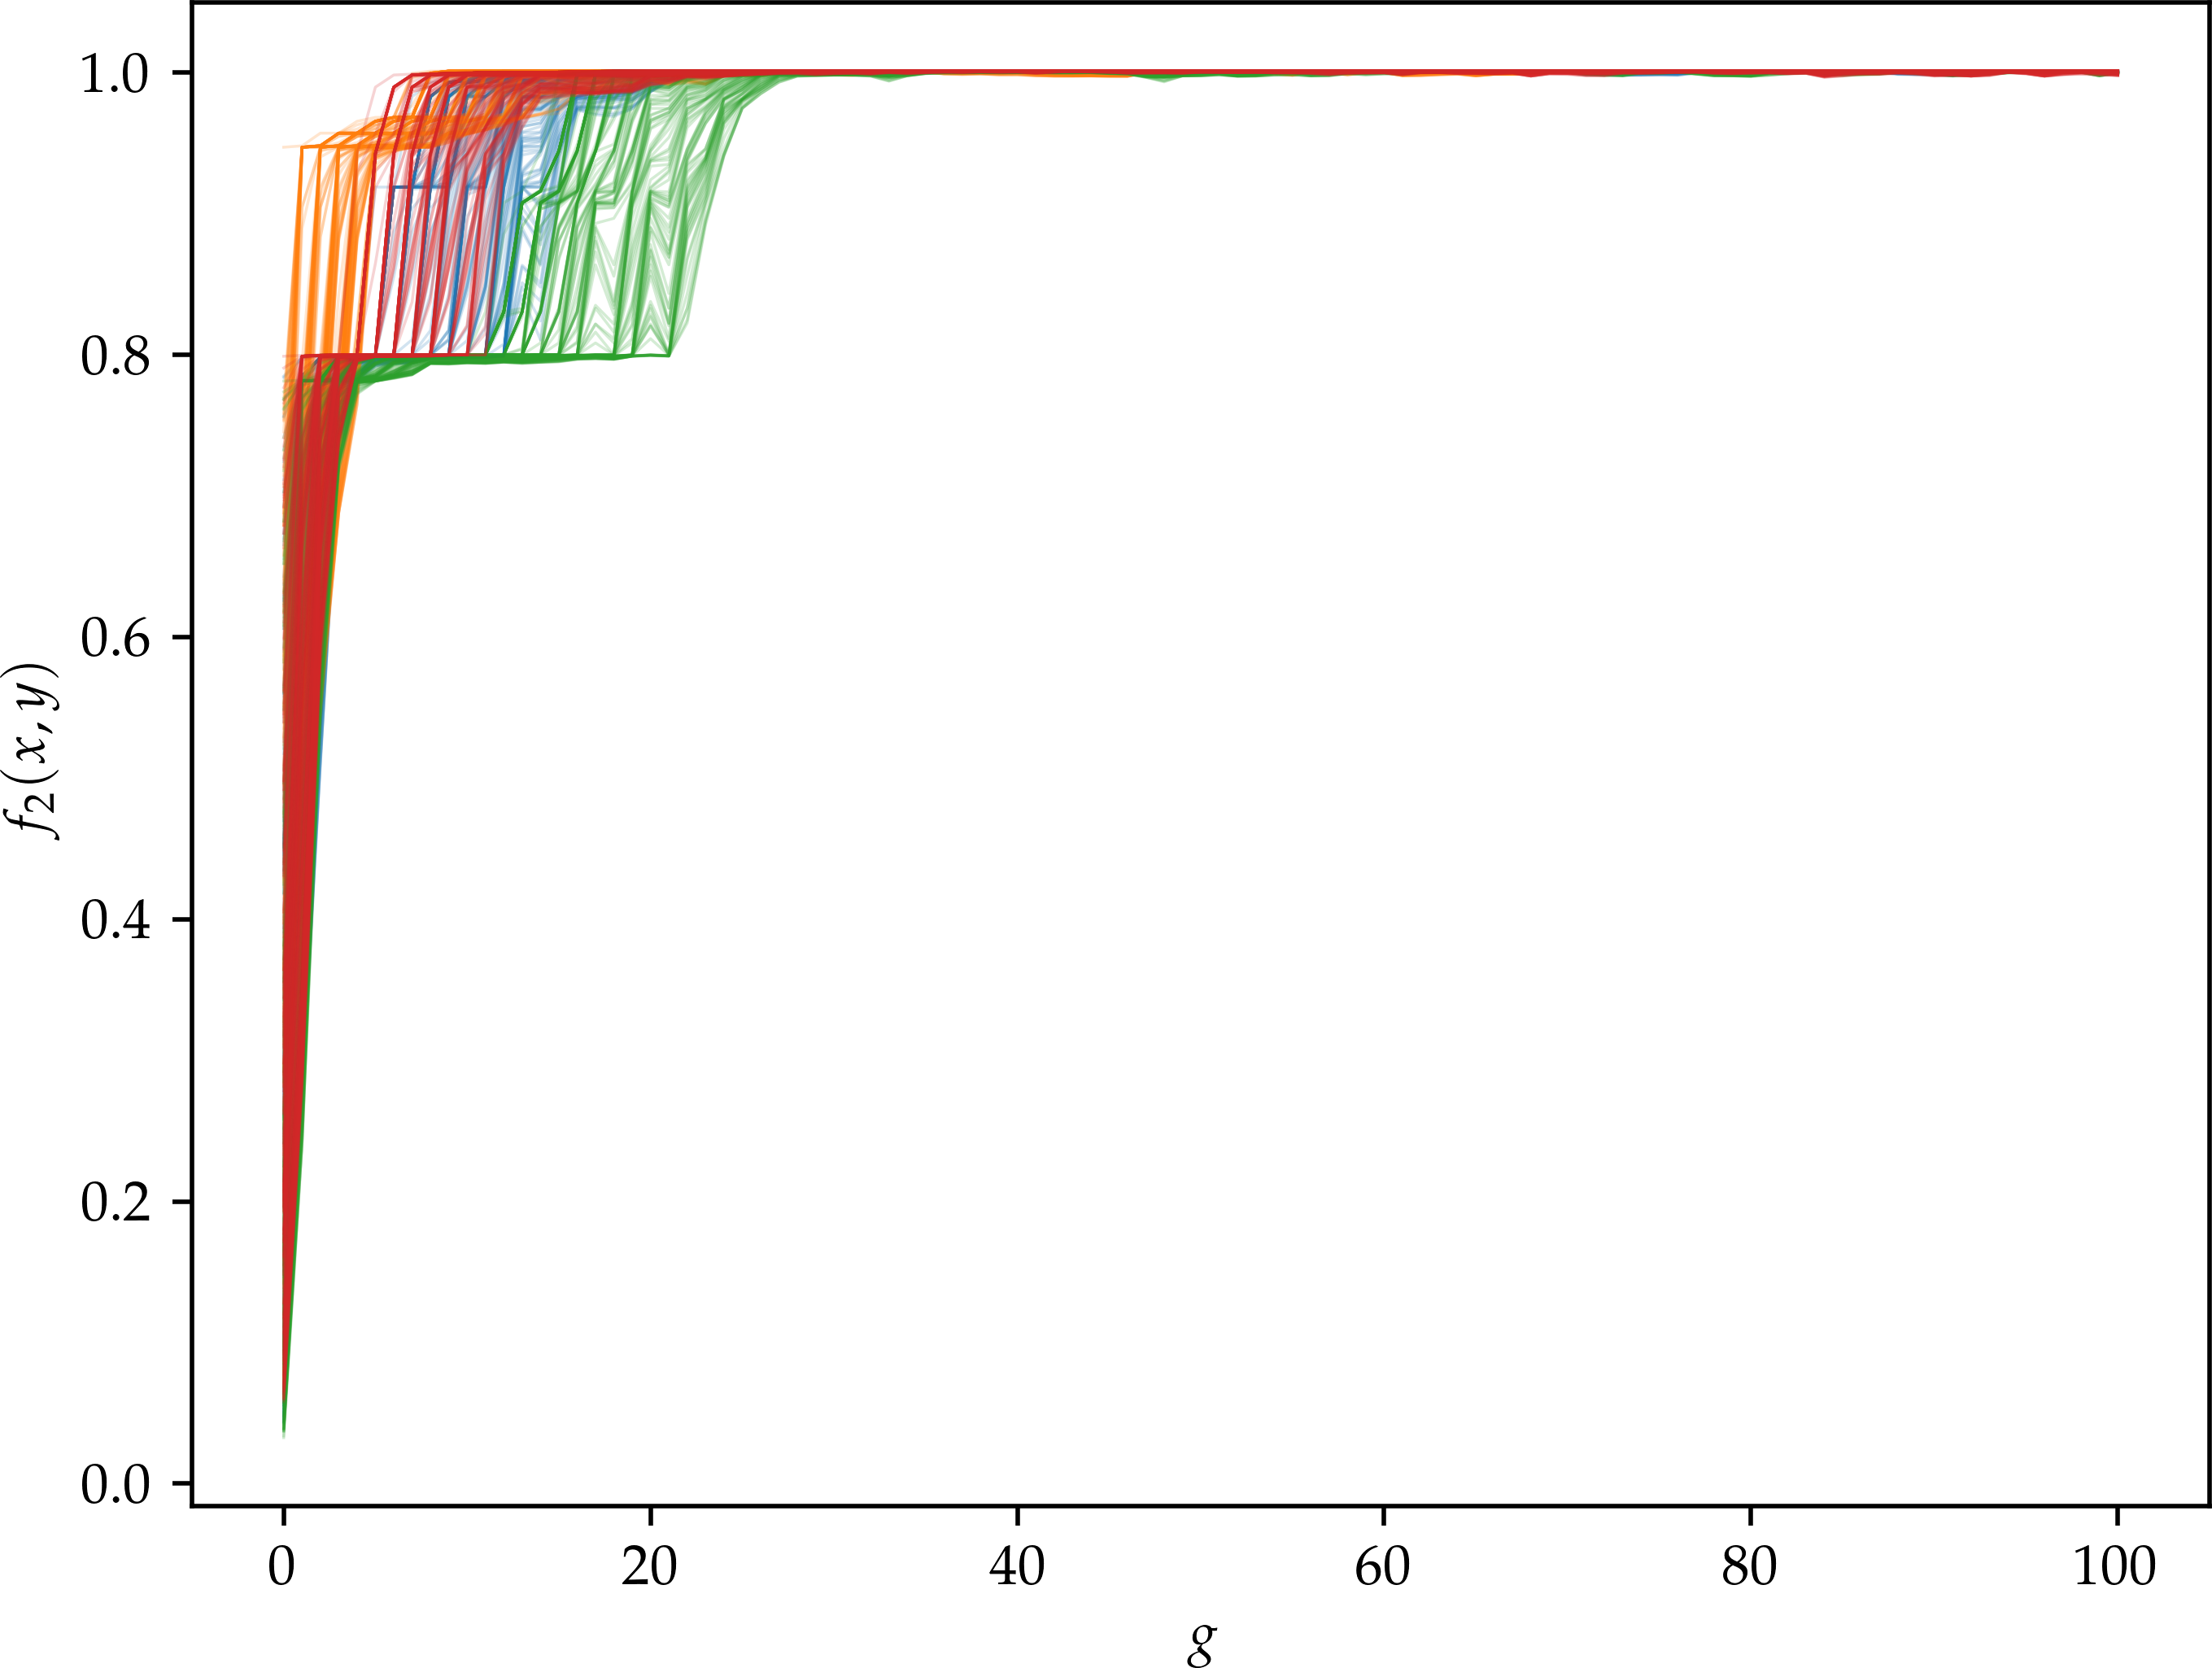
\includegraphics[width=\textwidth]{imagens/low_prob/evolution_near_gaussians.png}
  \caption{
    Evolução dos valores da função $ f_2(x,y) $ para os
    melhores 200 indivíduos de cada população, diferenciadas por cor, em termos da geração $g$,
    com $ p_2 = p_3 = 5\% $.
  }
  \label{fig:evolution_near_gaussians}
\end{figure}

\begin{figure}[p]
  \centering
  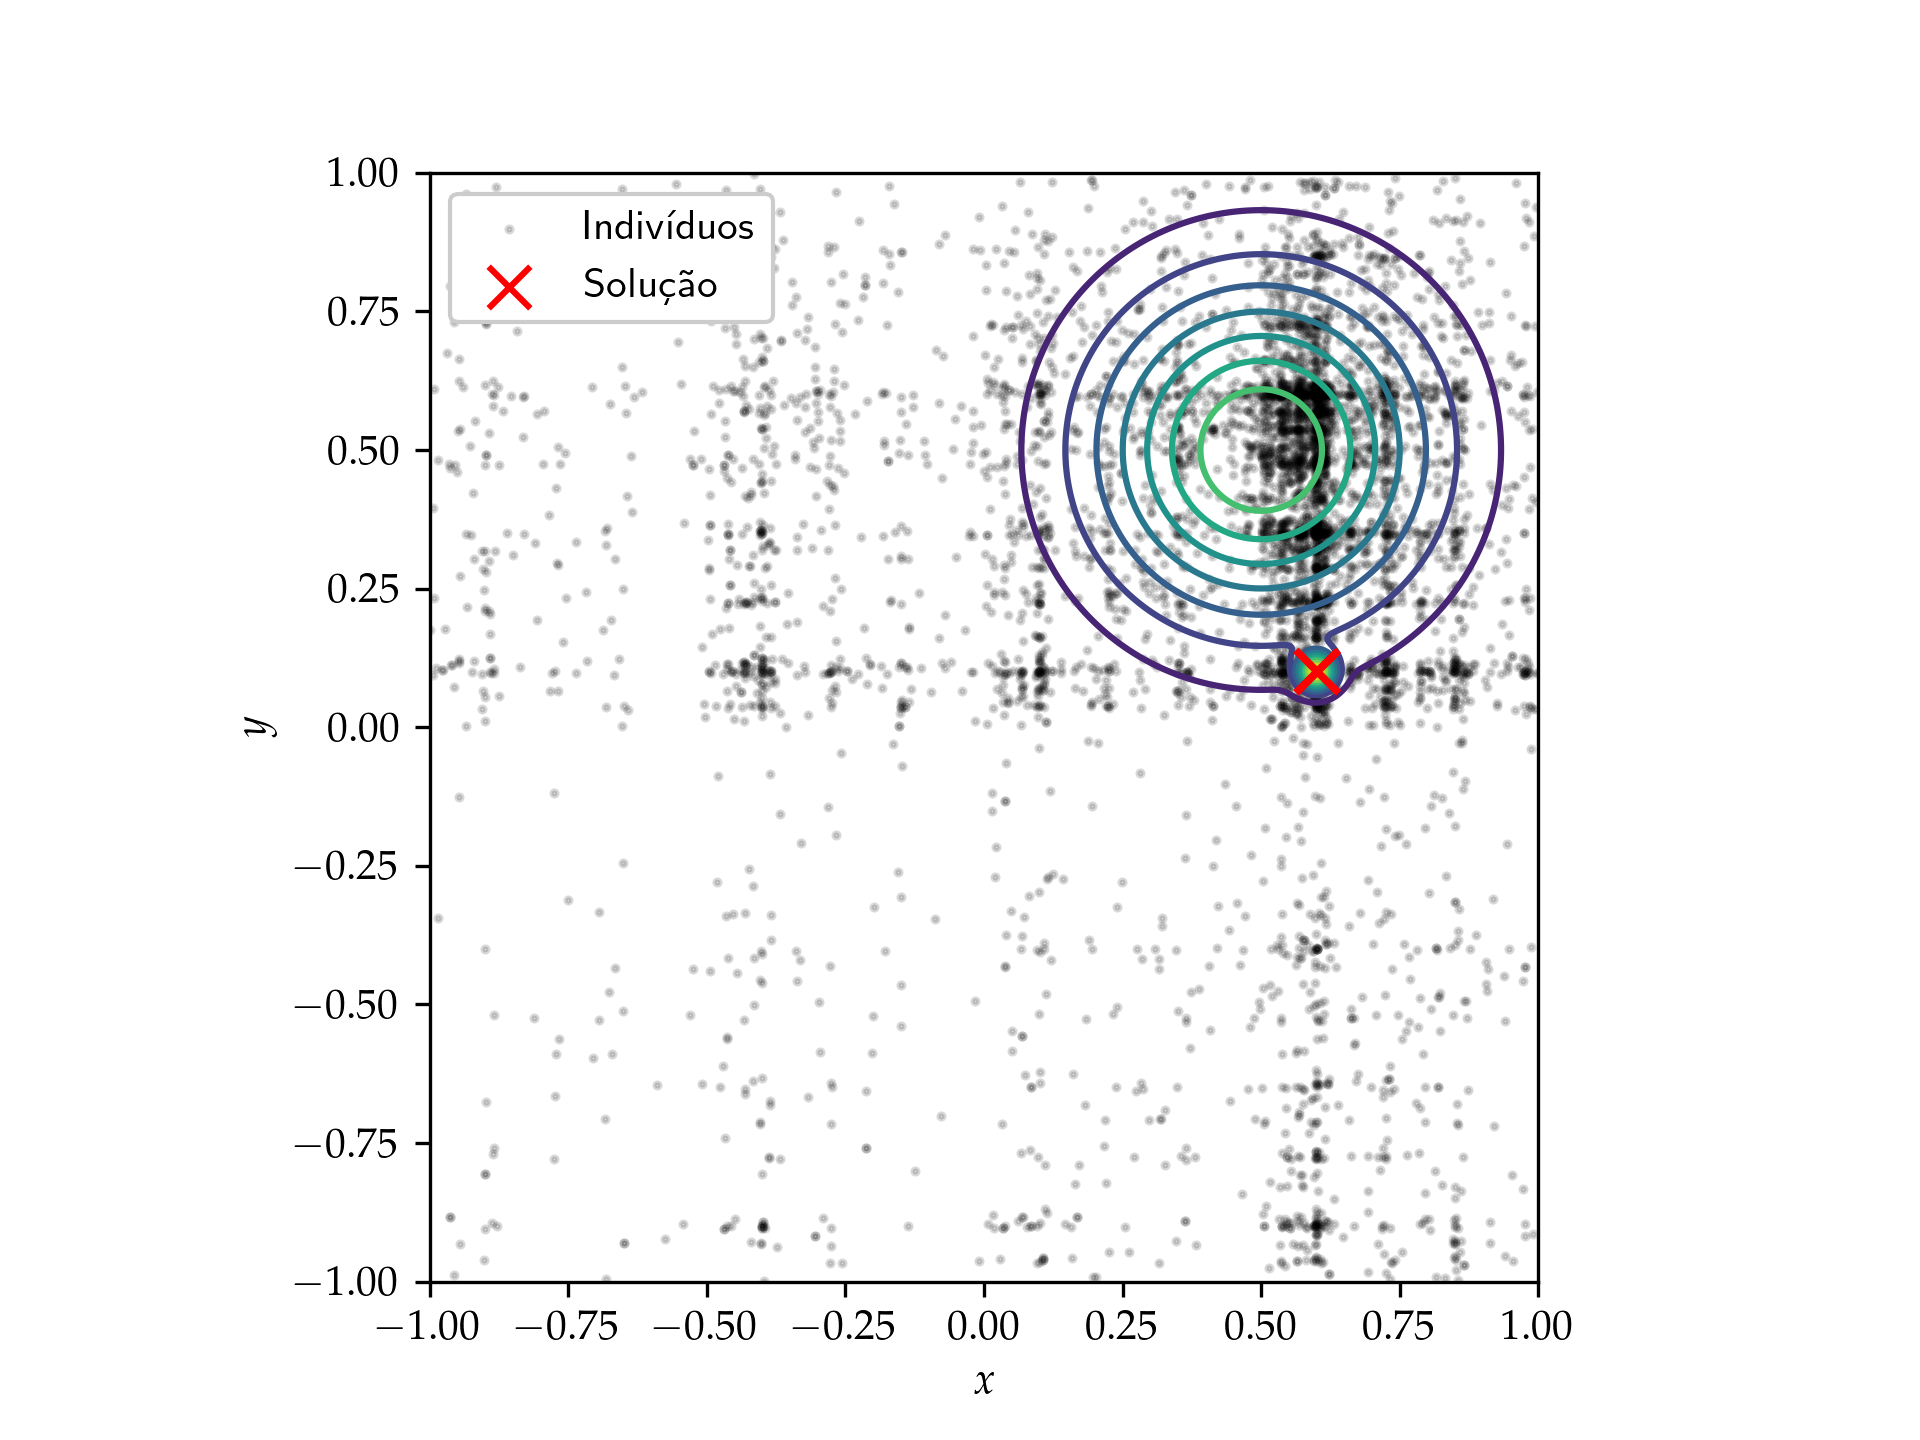
\includegraphics[width=\textwidth]{imagens/high_prob/contour_near_gaussians.png}
  \caption{
    Curvas de nível da função $f_2(x,y)$. Os pontos em preto indicam as posições dos indivíduos
    de 8 populações em sua 100ª geração na otimização da função, com $ p_2 = p_3 = 20\% $. 
    Marcado com um $\times$ vermelho estão os melhores indivíduos de cada população.
  }
  \label{fig:contour_near_gaussians_mut_20}
\end{figure}

\begin{figure}[p]
  \centering
  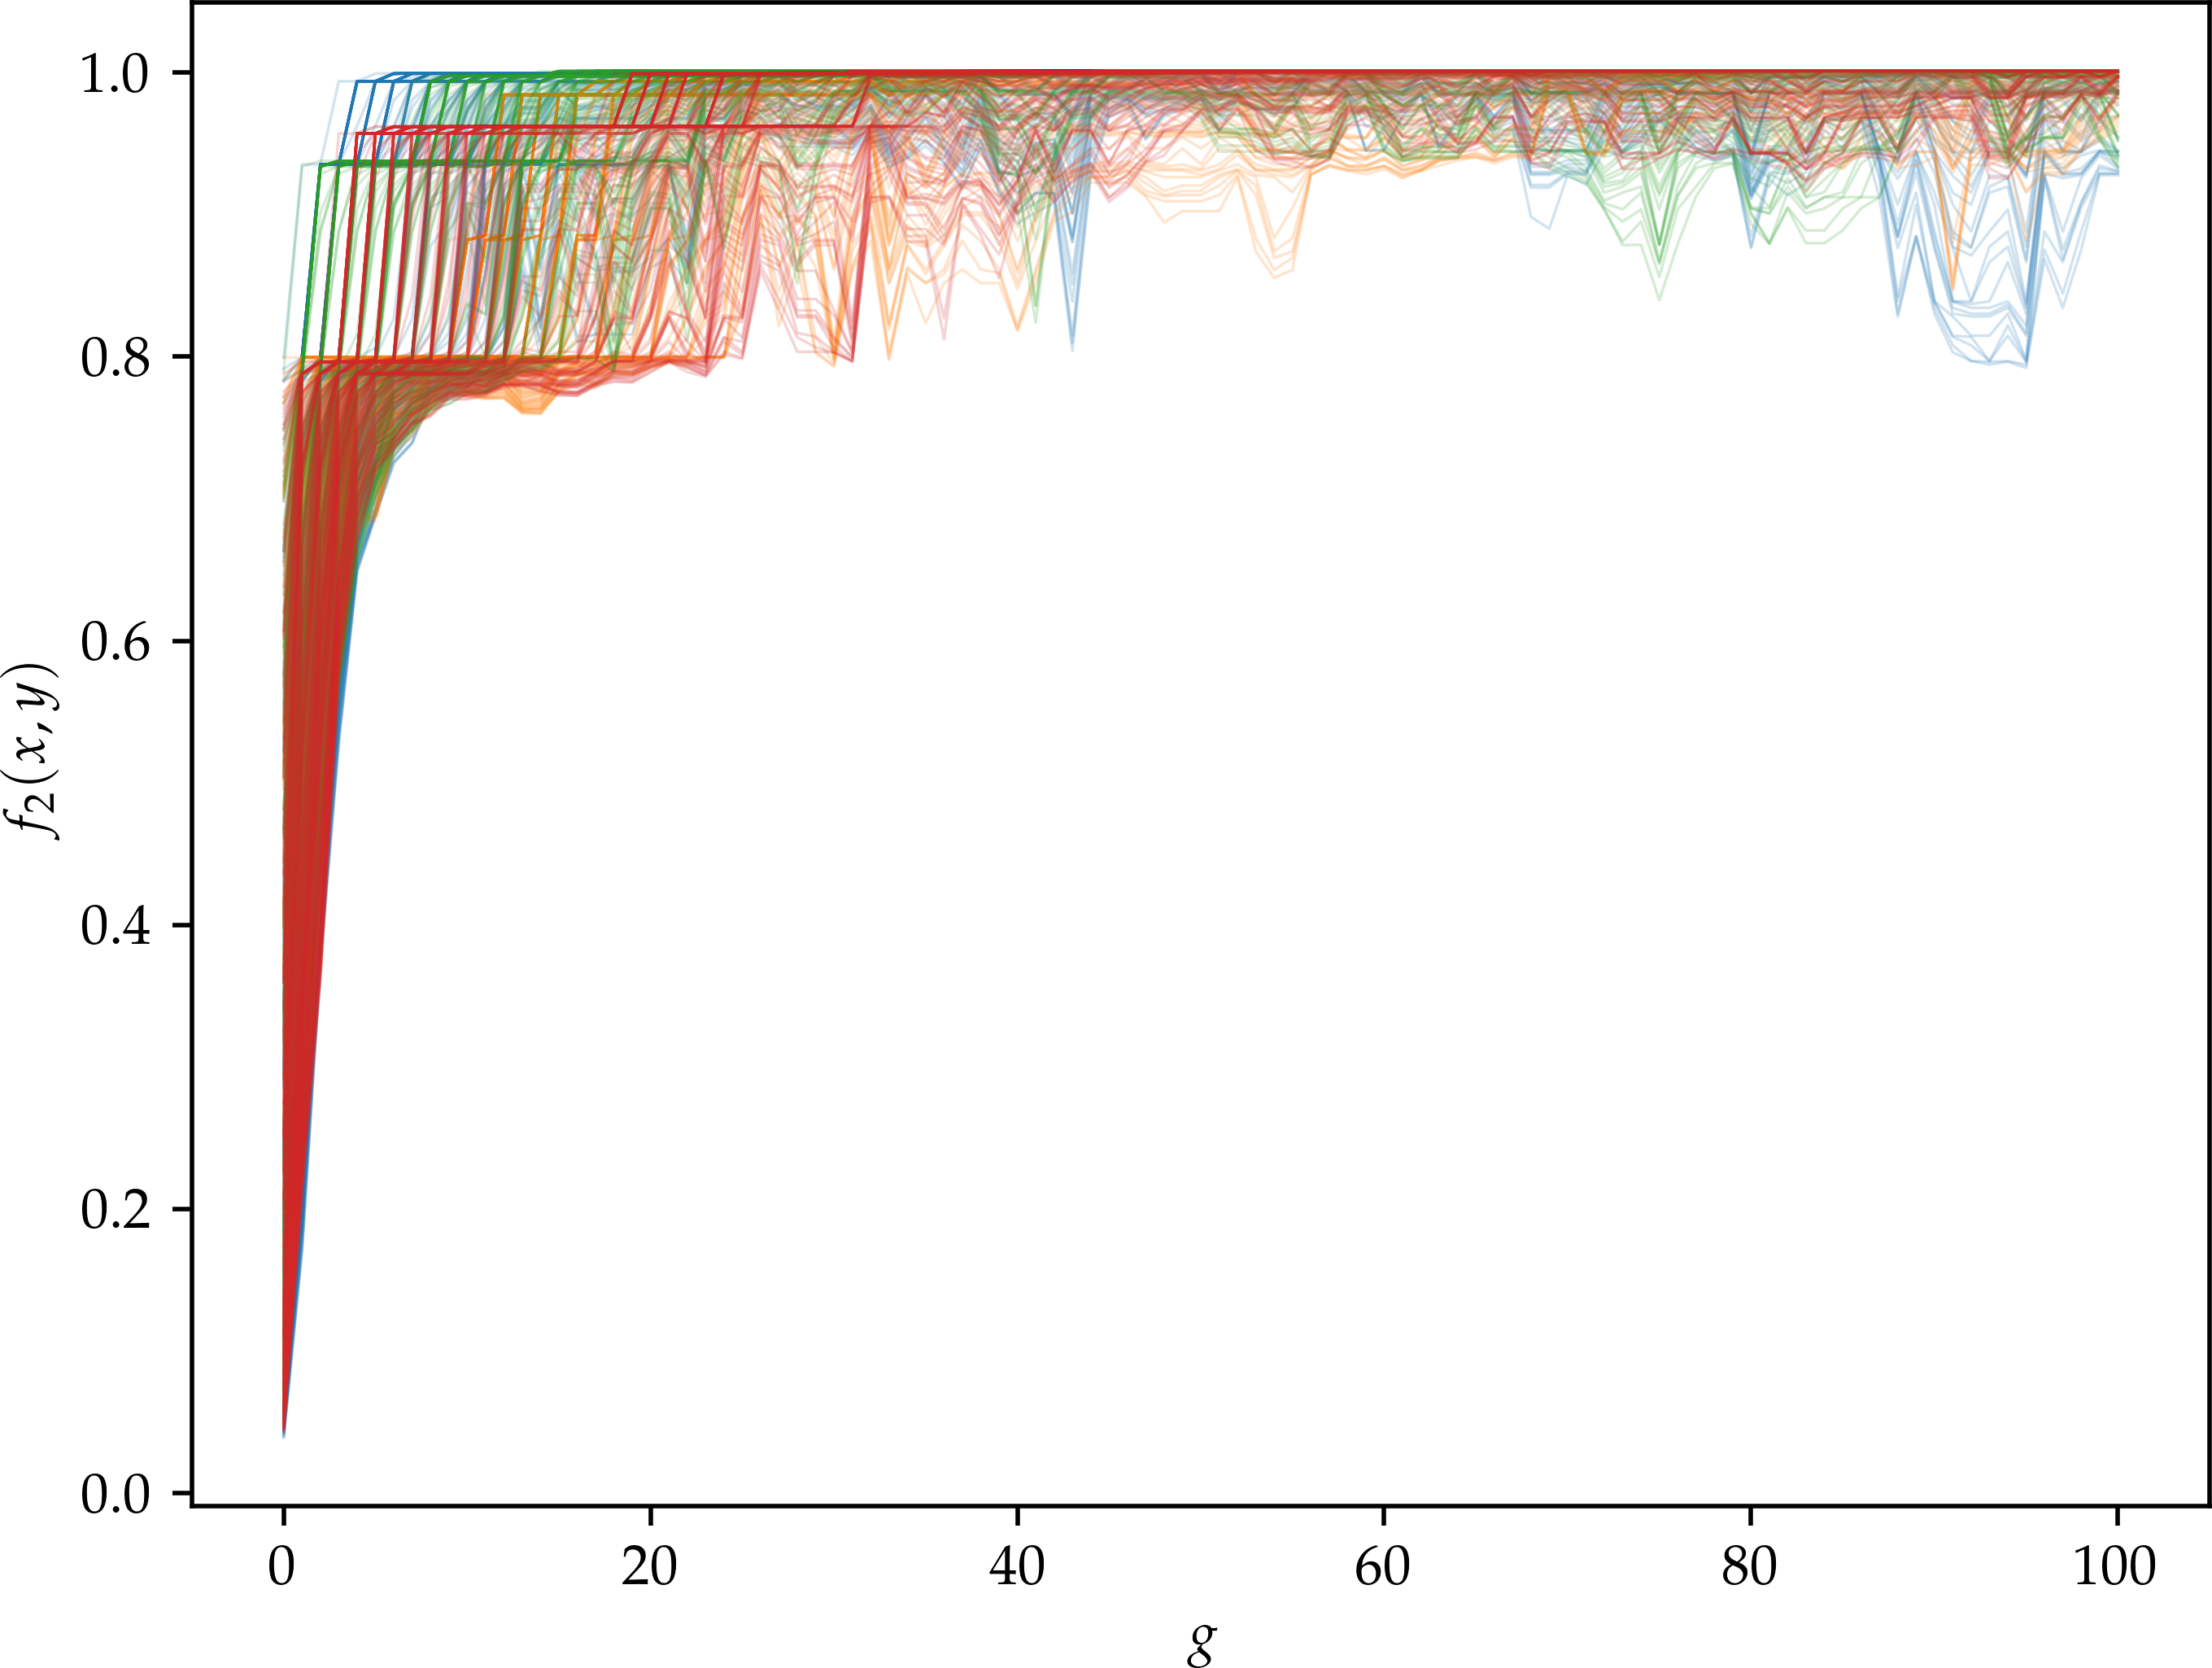
\includegraphics[width=\textwidth]{imagens/high_prob/evolution_near_gaussians.png}
  \caption{
    Evolução dos valores da função $ f_2(x,y) $ para os
    melhores 200 indivíduos de cada população, diferenciadas por cor, em termos da geração $g$,
    com $ p_2 = p_3 = 20\% $.
  }
  \label{fig:evolution_near_gaussians_mut_20}
\end{figure}

\section{Ajuste das Estruturas de Banda dos Cristais \ch{CrS2} e \ch{CrSe2}}
\label{sec_resultados_tmdcs}

Para o ajuste das bandas de energia dos materiais \ch{CrS2} e \ch{CrSe2} foram
executados 16 processos concorrentes com 1000 indivíduos cada, evoluídos no
decorrer de 200 gerações, com probabilidades de mutação $ p_2 = p_3 = 5\% $ e
$ h = 2 $. A distribuição da elite nas populações ocorreu de forma que $ e_1 =
  5\% $, $ e_2 = e_3 = 10\% $, sendo os percentuais tomados em relação ao tamanho
da população. A região de busca considerada no processo de ajuste é dada pelo
produto cartesiano dos intervalos na Tabela \ref{tab:search_region}.

É importante mencionar que foi usada uma estratégia para o refinamento do espaço
de busca, a qual consistiu em, após decorridas as primeiras 100 gerações, o
espaço de busca de cada população era limitado a um subespaço com 10\% do
volume, centrado no melhor indivíduo. Então novas populações eram
inicializadas\trav com uma distribuição uniforme de indivíduos na região
refinada\trav e o processo era retomado pelas 100 gerações restantes.
Ao final desse processo, toma-se o melhor indivíduo de todas as populações
como resultado.

\begin{table}[h]
  \centering
  \begin{tabular}{lrr}
    \toprule
                & $\xmin{j}$ & $\xmax{j}$ \\
    \midrule
    $E_F$       & \num{-1.0} & \num{1.0}  \\
    $\Delta$    & \num{0.5}  & \num{1.2}  \\
    $\lambda_c$ & \num{0.0}  & \num{1.0}  \\
    $\lambda_v$ & \num{0.0}  & \num{1.0}  \\
    $\gamma_i$  & \num{-1.0} & \num{1.0}  \\
    \bottomrule
  \end{tabular}
  \caption{
    Intervalos de busca para cada parâmetro considerados no ajuste das bandas de
    energia via modelo $ k \cdot p $. Definidos estes intervalos, a região de
    busca é calculada conforme a Equação \ref{eq:search_region}.
  }
  \label{tab:search_region}
\end{table}

Para fins de comparação, foi feito um ajuste da mesma função da Equação
\ref{eq:tmdc_obj_function} porém via outro método denominado
\textit{Dual Annealing}\footnote{
  Documentado em 
  \url{https://docs.scipy.org/doc/scipy/reference/generated/scipy.optimize.dual_annealing.html},
  com definição do modelo e respectivas referências enumeradas ao final da página.
}. Trata-se de um método também estocástico, com enfase em busca local e global,
assim como o Algoritmo Genético implementado. Para a busca, foi utilizado um
número máximo de iterações de 2000, e uma temperatura inicial 
$ T_{q_v}(1) = \num{2.5e4} $. Analogamente ao método anterior, tomamos para o
ajuste o melhor resultado de 16 processos concorrentes.

Quanto aos parâmetros relativos ao modelo $k \cdot p$, para
\ch{CrS2} e \ch{CrSe2}, os parâmetros de rede considerados para os cálculos, bem
como os valores esperados para $ \Delta $ se encontram enumerados na Tabela
\ref{tab:lattice_delta}. Para o metal de transição em questão, $ \eta = 1 $ e
uma vez que a expansão é feita em torno do ponto do vale $K$, $ \tau = 1 $.

\begin{table}[h]
  \centering
  \begin{tabular}{lcc}
    \toprule
                                       & \ch{CrS2}         & \ch{CrSe2}        \\
    \midrule
    $ a \; (\si{\angstrom}) $          & \num{3.022302679} & \num{3.167287237} \\
    $ \Delta \; (\si{\electronvolt}) $ & \num{0.942}       & \num{0.763}       \\
    \bottomrule
  \end{tabular}
  \caption{
    Valores para os parâmetros de rede considerados nos processos de otimização
    e valores esperados para o \textit{bandgap}, para cada um dos materiais
    considerados.
  }
  \label{tab:lattice_delta}
\end{table}

Os gráficos com os resultados obtidos por meio dos dois métodos utilizados
aplicados a cada um dos TMDCs se encontram nas Figuras \ref{fig:crs2} e
\ref{fig:crse2}, com os parâmetros ajustados detalhados nas Tabelas
\ref{tab:crs2} e \ref{tab:crse2}. Observando esses gráficos, é possível atestar
a eficácia de ambos os métodos de ajuste, uma vez que as bandas de energia da
expansão de 3ª ordem do modelo $k \cdot p$ praticamente coincidiram \trav na
vizinhança de $K$\trav com as bandas calculadas pelo método DFT\footnote{
  O cálculo DFT foi realizado utilizando o pacote Quantum Espresso, as equações de
  Kohn-Sham foram resolvidas utilizando uma base de ondas planas e projetores PAW
  \cite{paw1994} para tratar os elétrons do "caroço", sendo que foram utilizados projetores do
  tipo \textit{scalar relativistic} para optimização da estrutura e \textit{full relativistic}
  para o cálculo da estrutura de bandas. A optimização da estrutura  foi feita
  mediante a minimização do tensor de estresse, considerando a interação de van
  der Waals Grimme D3 \cite{grime2006} \cite{grimme2010}, utilizando o algoritmo
  BFGS \cite{bfgs_wiki06,bfgs_wiki07,bfgs_wiki08,bfgs_wiki09}
  e restringindo o grau de liberdade referente ao tamanho do vácuo da
  monocamada na direção z. Para isso utilizamos uma malha $ 16 \times 16 \times 1 $
  e as seguintes energias de corte para a base de ondas planas: 49 Ry
  para os três sistemas estudados. Os mesmos parâmetros de cálculo foram
  utilizados para as propriedades eletrônicas. 
}.

\begin{table}[p]
  \centering
  \begin{subtable}{\textwidth}
    \centering
    \begin{tabular}{lrrrr}
\toprule
{} & \multicolumn{2}{c}{Algorítmo Genético} & \multicolumn{2}{c}{\textit{Dual Annealing}} \\
{} &           1ª Ordem &  3ª Ordem &                1ª Ordem &  3ª Ordem \\
\midrule
$f$         &           0,003858 &  0,000335 &                0,003860 &  0,000165 \\
$E_F$       &          -0,052734 &  0,023191 &               -0,052109 &  0,010791 \\
$\Delta$    &           1,077500 &  0,954347 &                1,076284 &  0,976370 \\
$\lambda_c$ &          -0,002289 &  0,006503 &                0,000000 &  0,000000 \\
$\lambda_v$ &           0,031810 &  0,030079 &                0,032250 &  0,033154 \\
$\gamma_0$  &           0,475147 &  0,508048 &               -0,475765 &  0,662441 \\
$\gamma_1$  &                    &  0,227823 &                         &  0,038586 \\
$\gamma_2$  &                    & -0,216329 &                         & -0,050962 \\
$\gamma_3$  &                    &  0,185349 &                         &  0,196977 \\
$\gamma_4$  &                    & -0,063952 &                         & -0,128763 \\
$\gamma_5$  &                    &  0,037538 &                         &  0,116953 \\
$\gamma_6$  &                    & -0,196858 &                         & -0,147924 \\
\bottomrule
\end{tabular}

    \caption{}
    \label{tab:crs2}
  \end{subtable}
  \\
  \vspace{0.6cm}
  \begin{subtable}{\textwidth}
    \centering
    \begin{tabular}{lrrrr}
\toprule
{} & \multicolumn{2}{c}{Algorítmo Genético} & \multicolumn{2}{c}{\textit{Dual Annealing}} \\
{} &           1ª Ordem &  3ª Ordem &                1ª Ordem &  3ª Ordem \\
\midrule
$f$         &           0,002695 &  0,000261 &                0,002695 &  0,000129 \\
$E_F$       &           0,657808 &  0,722708 &                0,657704 &  0,715254 \\
$\Delta$    &           0,897031 &  0,792868 &                0,896809 &  0,814547 \\
$\lambda_c$ &           0,006592 &  0,007456 &                0,006680 &  0,007329 \\
$\lambda_v$ &           0,045311 &  0,047549 &                0,045330 &  0,042298 \\
$\gamma_0$  &          -0,381442 & -0,649511 &                0,381519 &  0,456269 \\
$\gamma_1$  &                    & -0,090387 &                         &  0,137704 \\
$\gamma_2$  &                    &  0,090028 &                         & -0,154747 \\
$\gamma_3$  &                    & -0,075382 &                         &  0,124848 \\
$\gamma_4$  &                    & -0,059988 &                         & -0,030592 \\
$\gamma_5$  &                    &  0,037979 &                         &  0,016737 \\
$\gamma_6$  &                    &  0,110312 &                         & -0,169387 \\
\bottomrule
\end{tabular}

    \caption{}
    \label{tab:crse2}
  \end{subtable}
  \caption{
    Parâmetros da hamiltoniana $ \hat{H}_{kp} $ ajustados para \ch{CrS2} \subref{tab:crs2}
    e para \ch{CrSe2} \subref{tab:crse2} usando as expansões de 1ª e 3ª ordem
    de $ \hat{H}_{kp} $, bem como os valores para a função objetivo $f$ correspondente.
  }
  \label{tab:fit_results}
\end{table}

O \textit{bandgap} estimado com ambos os métodos apresentou uma discrepância
menor que 5\% com relação ao valor esperado para a expansão de 3ª ordem, o que
atesta a eficácia de ambos os métodos e do modelo $ k \cdot p $ em si. Ademais,
é possível observar que os valores obtidos para os parâmetros $E_F$, $\Delta$,
$\lambda_c$ e $\lambda_v$ e para o valor mínimo de $f$ encontrado em ambas as
ordens utilizadas não apresentaram grande discrepância quando comparados entre
os dois métodos utilizados para a busca. Já o parâmetro $\gamma_0$ ajustado
também apresentou uma variação muito pequena, porém com uma troca de sinal.

Dito isso, pode-se agora fazer uso prático dos parâmetros ajustados. Como
enunciado na Seção \ref{sec_tmdcs_intro}, o modelo $ k \cdot p $ possibilita a
inclusão de um termo de interação referente a um campo magnético uniforme 
$ \bvec{B} = B e_z $ à hamiltoniana $ \hat{H}_{kp} $. Assim, os novos níveis de
energia das bandas de valência e de condução serão dados pelos novos
autovalores. Calculando-os para a expansão de 1ª ordem obteremos as energias
\begin{equation}
  E_\pm (B, n, s_z) = \frac{\lambda_v \tau s_z}{2} \pm 
  \sqrt{
    \frac{(\Delta - \lambda_v \tau s_z)^2}{4} + 
    \frac{2 \gamma_0^2 a^2 e B n}{\hbar}
  }
  \mathcomma
  \label{eq:landau_levels}
\end{equation}
onde os sinais $+$ e $-$ se referem, respectivamente, as bandas de condução e de
valência, e $ s_z = 1 $ e $ s_z = -1 $ representam estados de spin \textit{up} e
\textit{down}, e $n$ é um natural não nulo \cite{dias2016tmdc,dias2016article,rose2013}. Para o caso
particular em que $ n = 0 $, 
\begin{equation}
  E_{n = 0} =
  \begin{cases}
    - \nicefrac{\Delta}{2} + \lambda_v s_z \;, & \text{se } \tau = 1  \\
    \nicefrac{\Delta}{2}                   \;, & \text{se } \tau = -1 \\
  \end{cases}
  \label{eq:landau_level_for_null_n}
\end{equation}
correspondendo a níveis de valência e de condução.

Os gráficos das Figuras \ref{fig:crs2_k_valley_landau_levels} e
\ref{fig:crse2_k_valley_landau_levels} ilustram o novo comportamento das bandas
de condução e de valência no vale $K$ para ambos os materiais estudados: com a
presença de um campo externo, há a quebra de degenerescência dando origem a
novos níveis de energia, conhecidos como níveis de Landau. De forma similar, nas
Figuras \ref{fig:crs2_k_prime_valley_landau_levels} e
\ref{fig:crse2_k_prime_valley_landau_levels} é retratado esse mesmo fenômeno
para o vale $K'$\footnote{
  É importante frisar que nas Figuras \ref{fig:k_valley_landau_levels} e
  \ref{fig:k_prime_valley_landau_levels}, o nível de referência de energia difere
  dos utilizados nas Figuras \ref{fig:crs2} e \ref{fig:crse2}.
}.

Como consequência, o \textit{bandgap} do material também será dependente de $B$ de forma que
\begin{equation}
  \Delta(B) = 
  \begin{cases}
    E_+(B, 1, -1) - \left( \lambda_v - \nicefrac{\Delta}{2} \right) \;, & \text{se } \tau = 1  \\
    \nicefrac{\Delta}{2} - E_-(B, 1, -1) \;,                            & \text{se } \tau = -1 \\
  \end{cases}
  \mathcomma
  \label{eq:new_bandgap}
\end{equation}
havendo a quebra da simetria entre os valores calculados para os vales $K$ e
$K'$, como é destacado nas Figuras \ref{fig:crs2_bandgap_field} e
\ref{fig:crse2_bandgap_field}. Tal comportamento pode ser explorado em
aplicações, uma vez que quanto maior o campo externo, maior é a dificuldade na
criação de um exciton, o que respalda em uma menor capacidade condutiva do
material.  

Isso pode criar margem para aplicações similares a sensores do tipo Hall, os quais
também tem por princípio o controle da condutividade com a aplicação de um campo
magnético externo.

\begin{figure}[p]
  \centering
  \begin{subfigure}{\textwidth}
    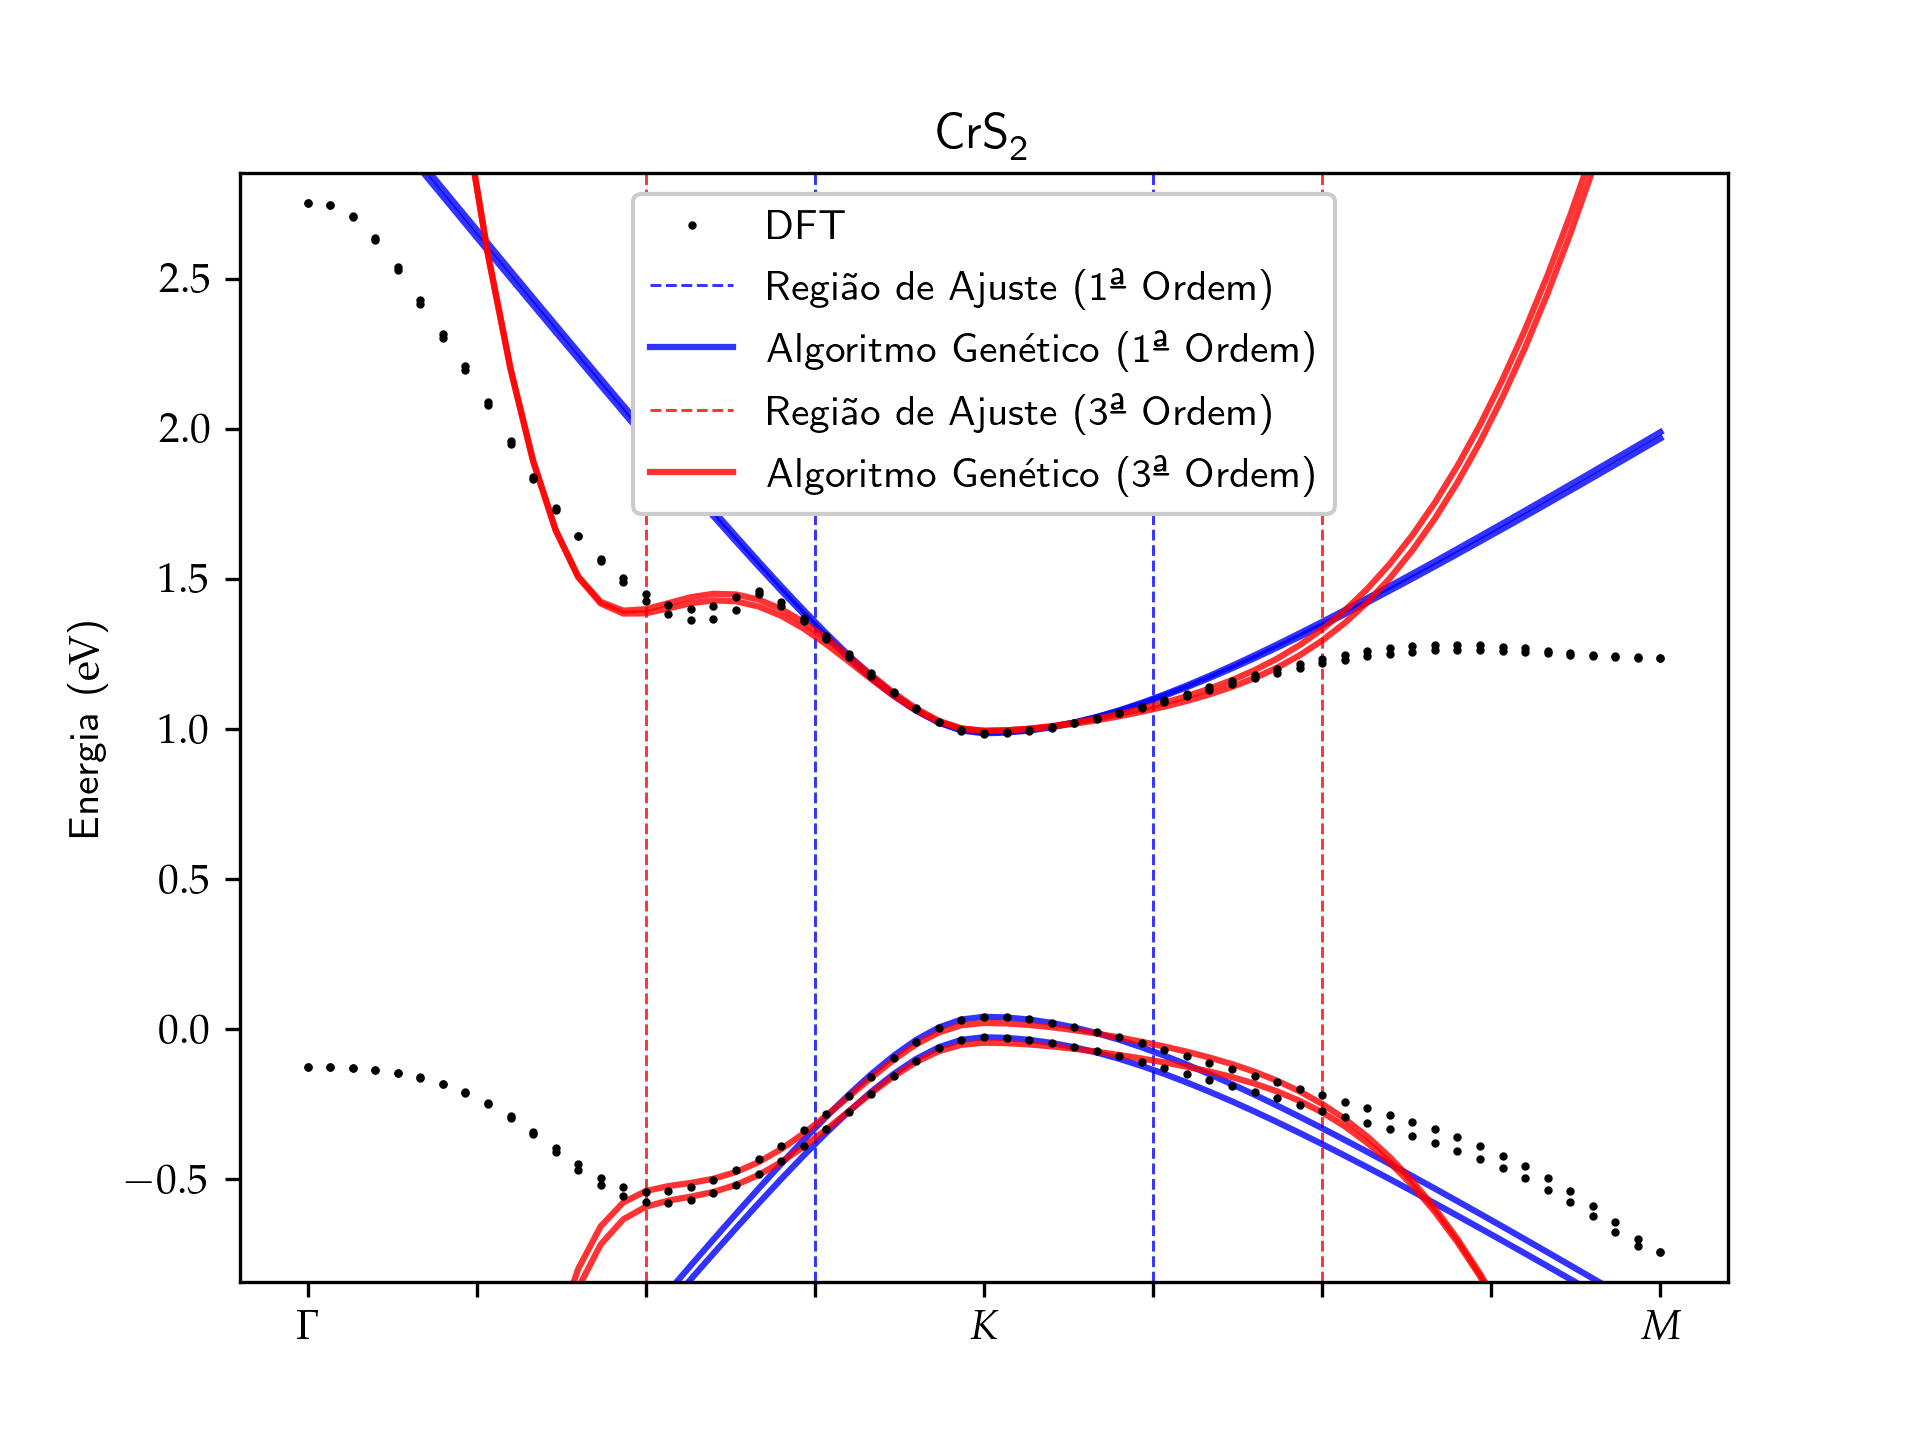
\includegraphics[trim=0 0.6cm 0 0.6cm,clip,width=\textwidth]{imagens/crs2_genetic_algorithm_order_13.png}
    \caption{}
    \label{fig:crs2_genetic_algorithm}
  \end{subfigure}
  \begin{subfigure}{\textwidth}
    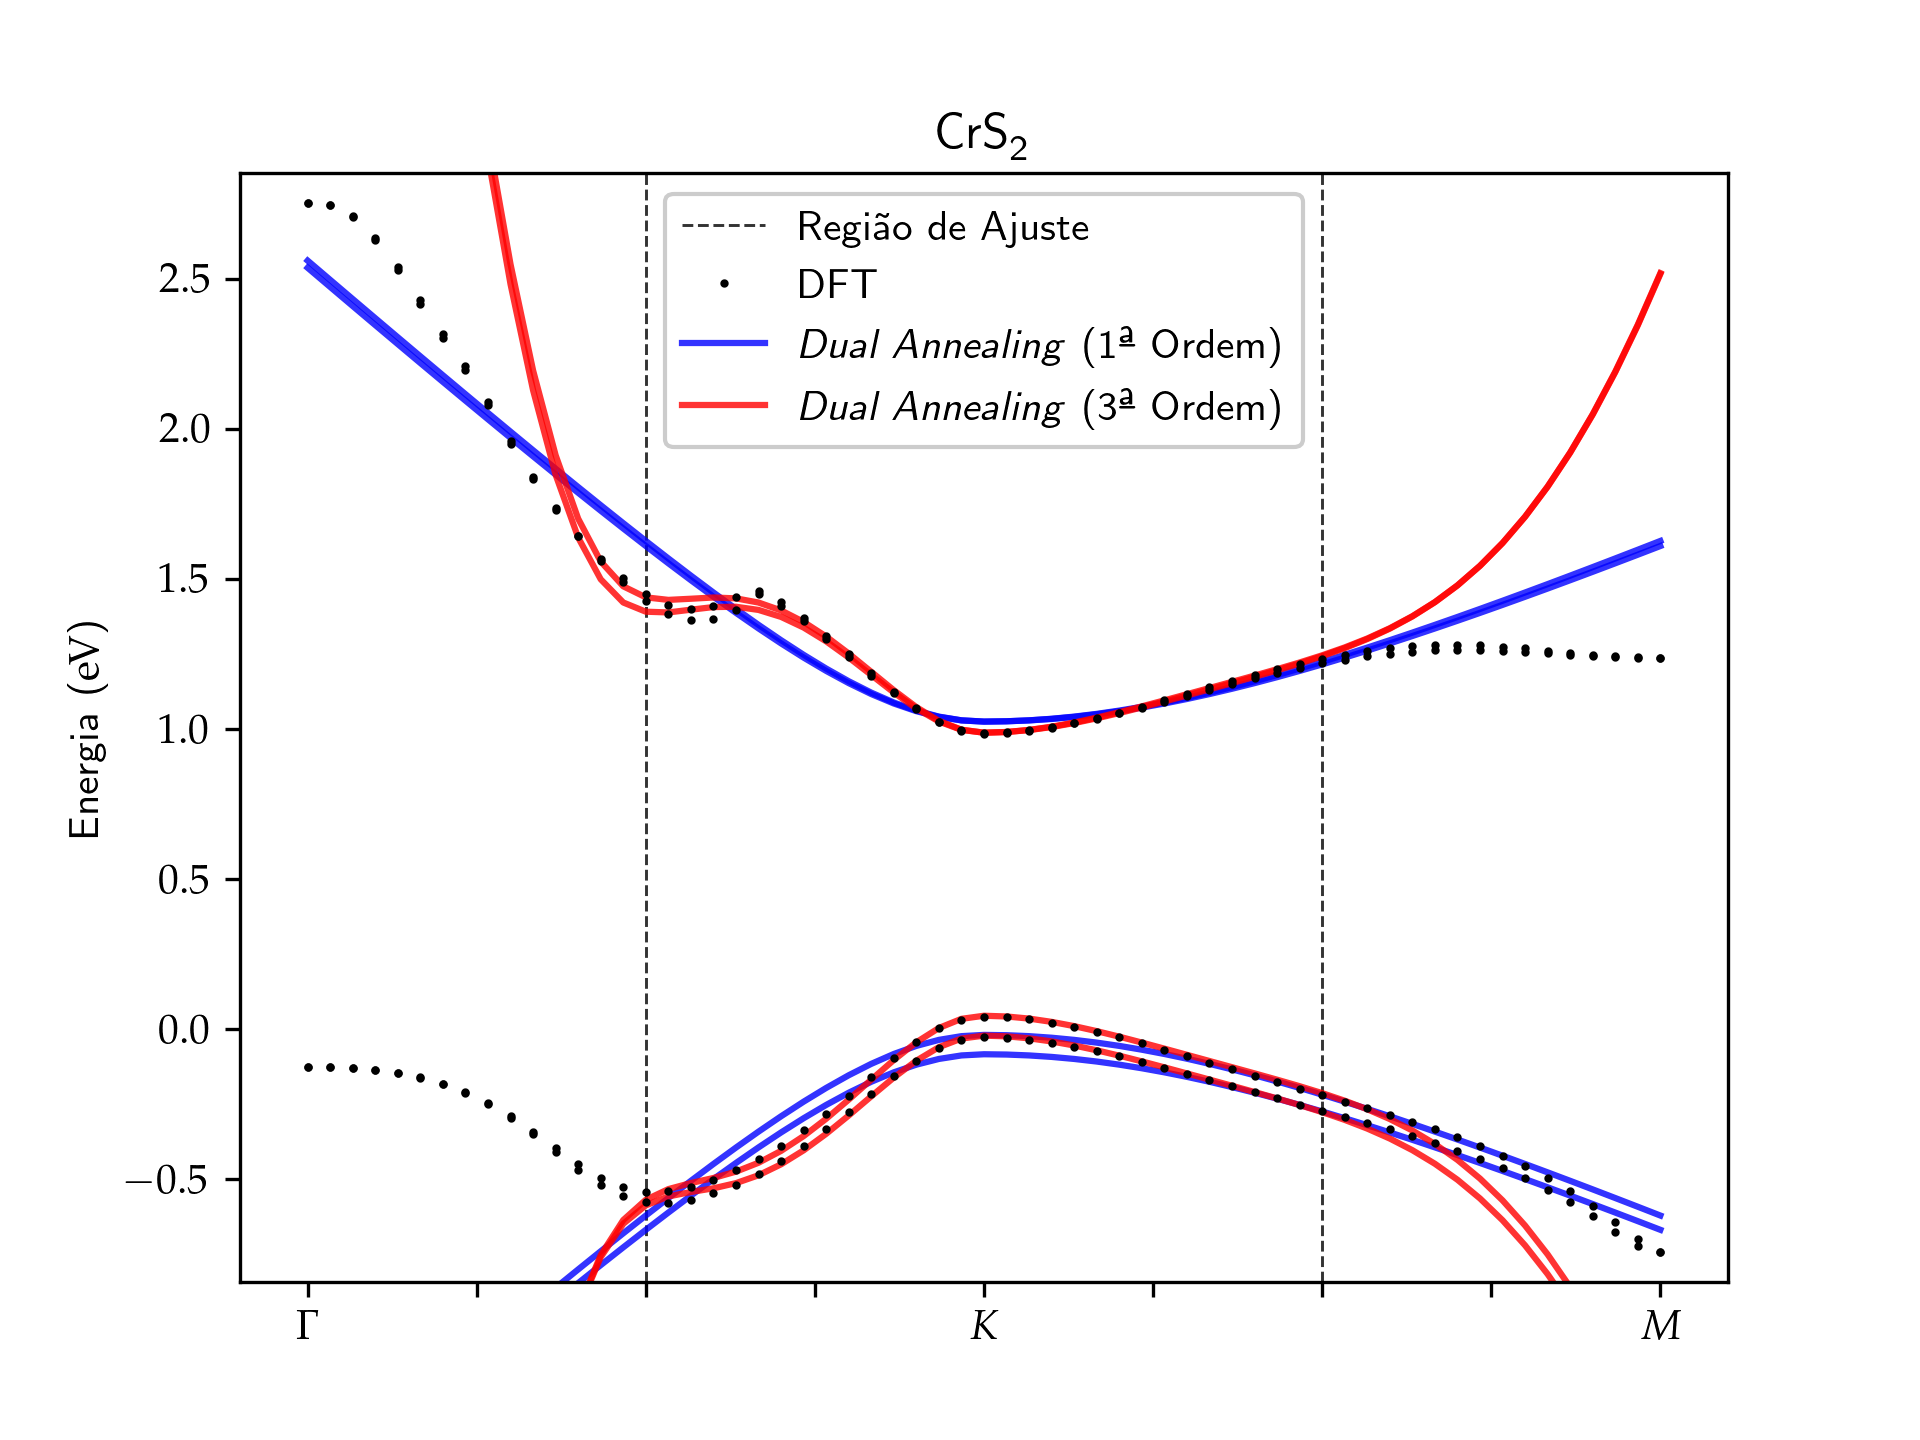
\includegraphics[trim=0 0.6cm 0 0.6cm,clip,width=\textwidth]{imagens/crs2_dual_annealing_order_13.png}
    \caption{}
    \label{fig:crs2_dual_annealing}
  \end{subfigure}
  \caption{
    Gráficos das bandas de energia ajustadas para \ch{CrS2} via Algoritmo Genético
    \subref{fig:crs2_genetic_algorithm} e via \textit{Dual Annealing} \subref{fig:crs2_dual_annealing}
    usando as expansões de 1ª e 3ª ordem de $ \hat{H}_{kp} $.
  }
  \label{fig:crs2}
\end{figure}

\begin{figure}[p]
  \centering
  \begin{subfigure}{\textwidth}
    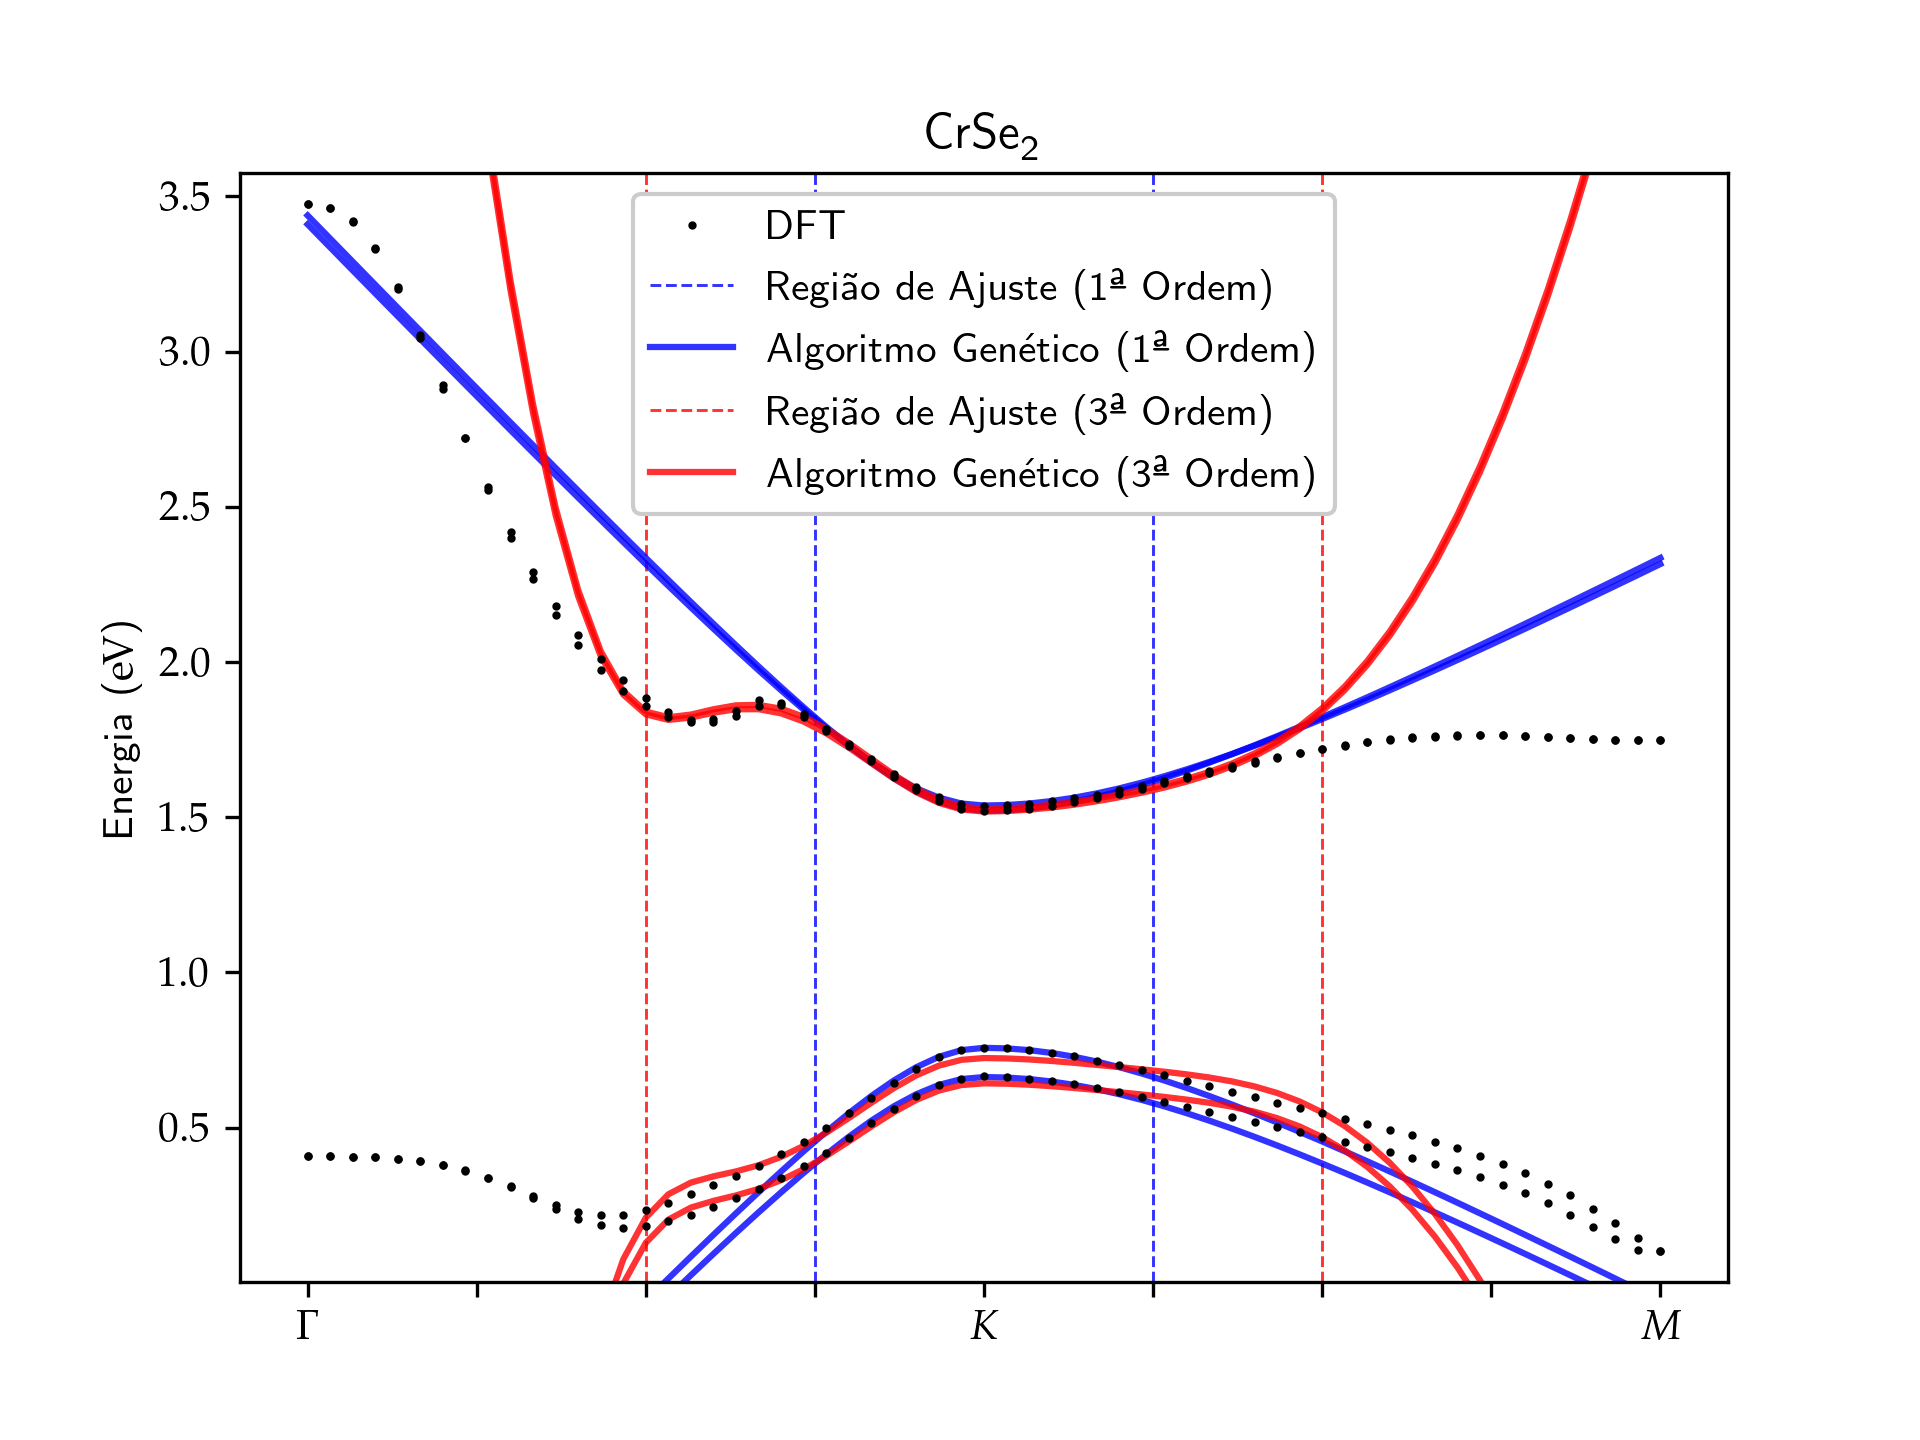
\includegraphics[trim=0 0.6cm 0 0.6cm,clip,width=\textwidth]{imagens/crse2_genetic_algorithm_order_13.png}
    \caption{}
    \label{fig:crse2_genetic_algorithm}
  \end{subfigure}
  \begin{subfigure}{\textwidth}
    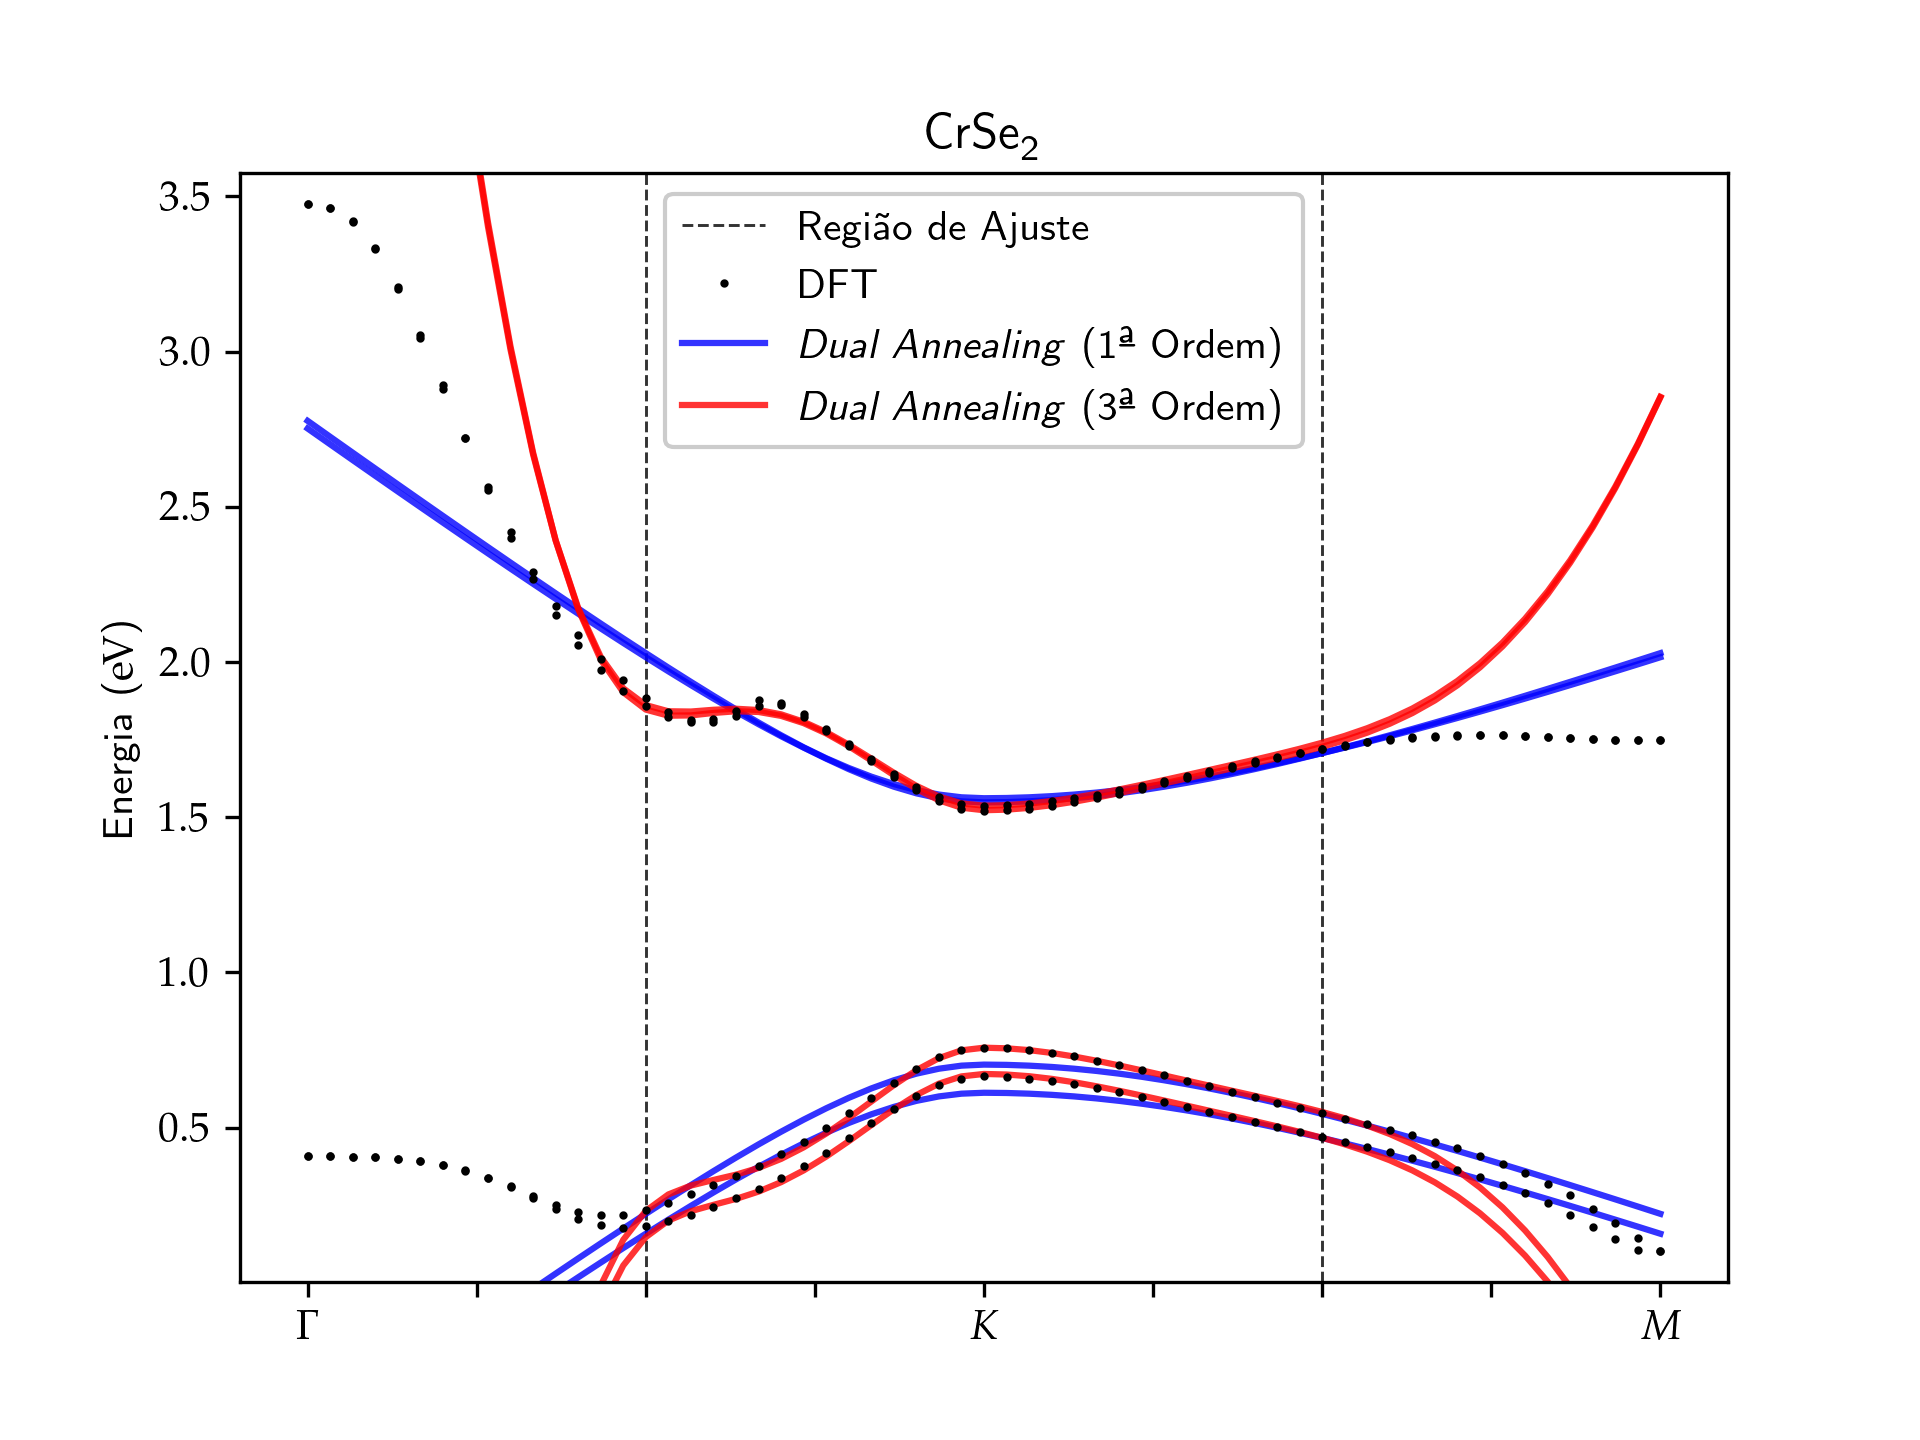
\includegraphics[trim=0 0.6cm 0 0.6cm,clip,width=\textwidth]{imagens/crse2_dual_annealing_order_13.png}
    \caption{}
    \label{fig:crse2_dual_annealing}
  \end{subfigure}
  \caption{
    Gráficos das bandas de energia ajustadas para \ch{CrSe2} via Algoritmo Genético
    \subref{fig:crse2_genetic_algorithm} e via \textit{Dual Annealing}
    \subref{fig:crse2_dual_annealing} usando as expansões de 1ª e 3ª ordem de $ \hat{H}_{kp} $.
  }
  \label{fig:crse2}
\end{figure}

\begin{figure}[p]
  \centering
  \begin{subfigure}{\textwidth}
    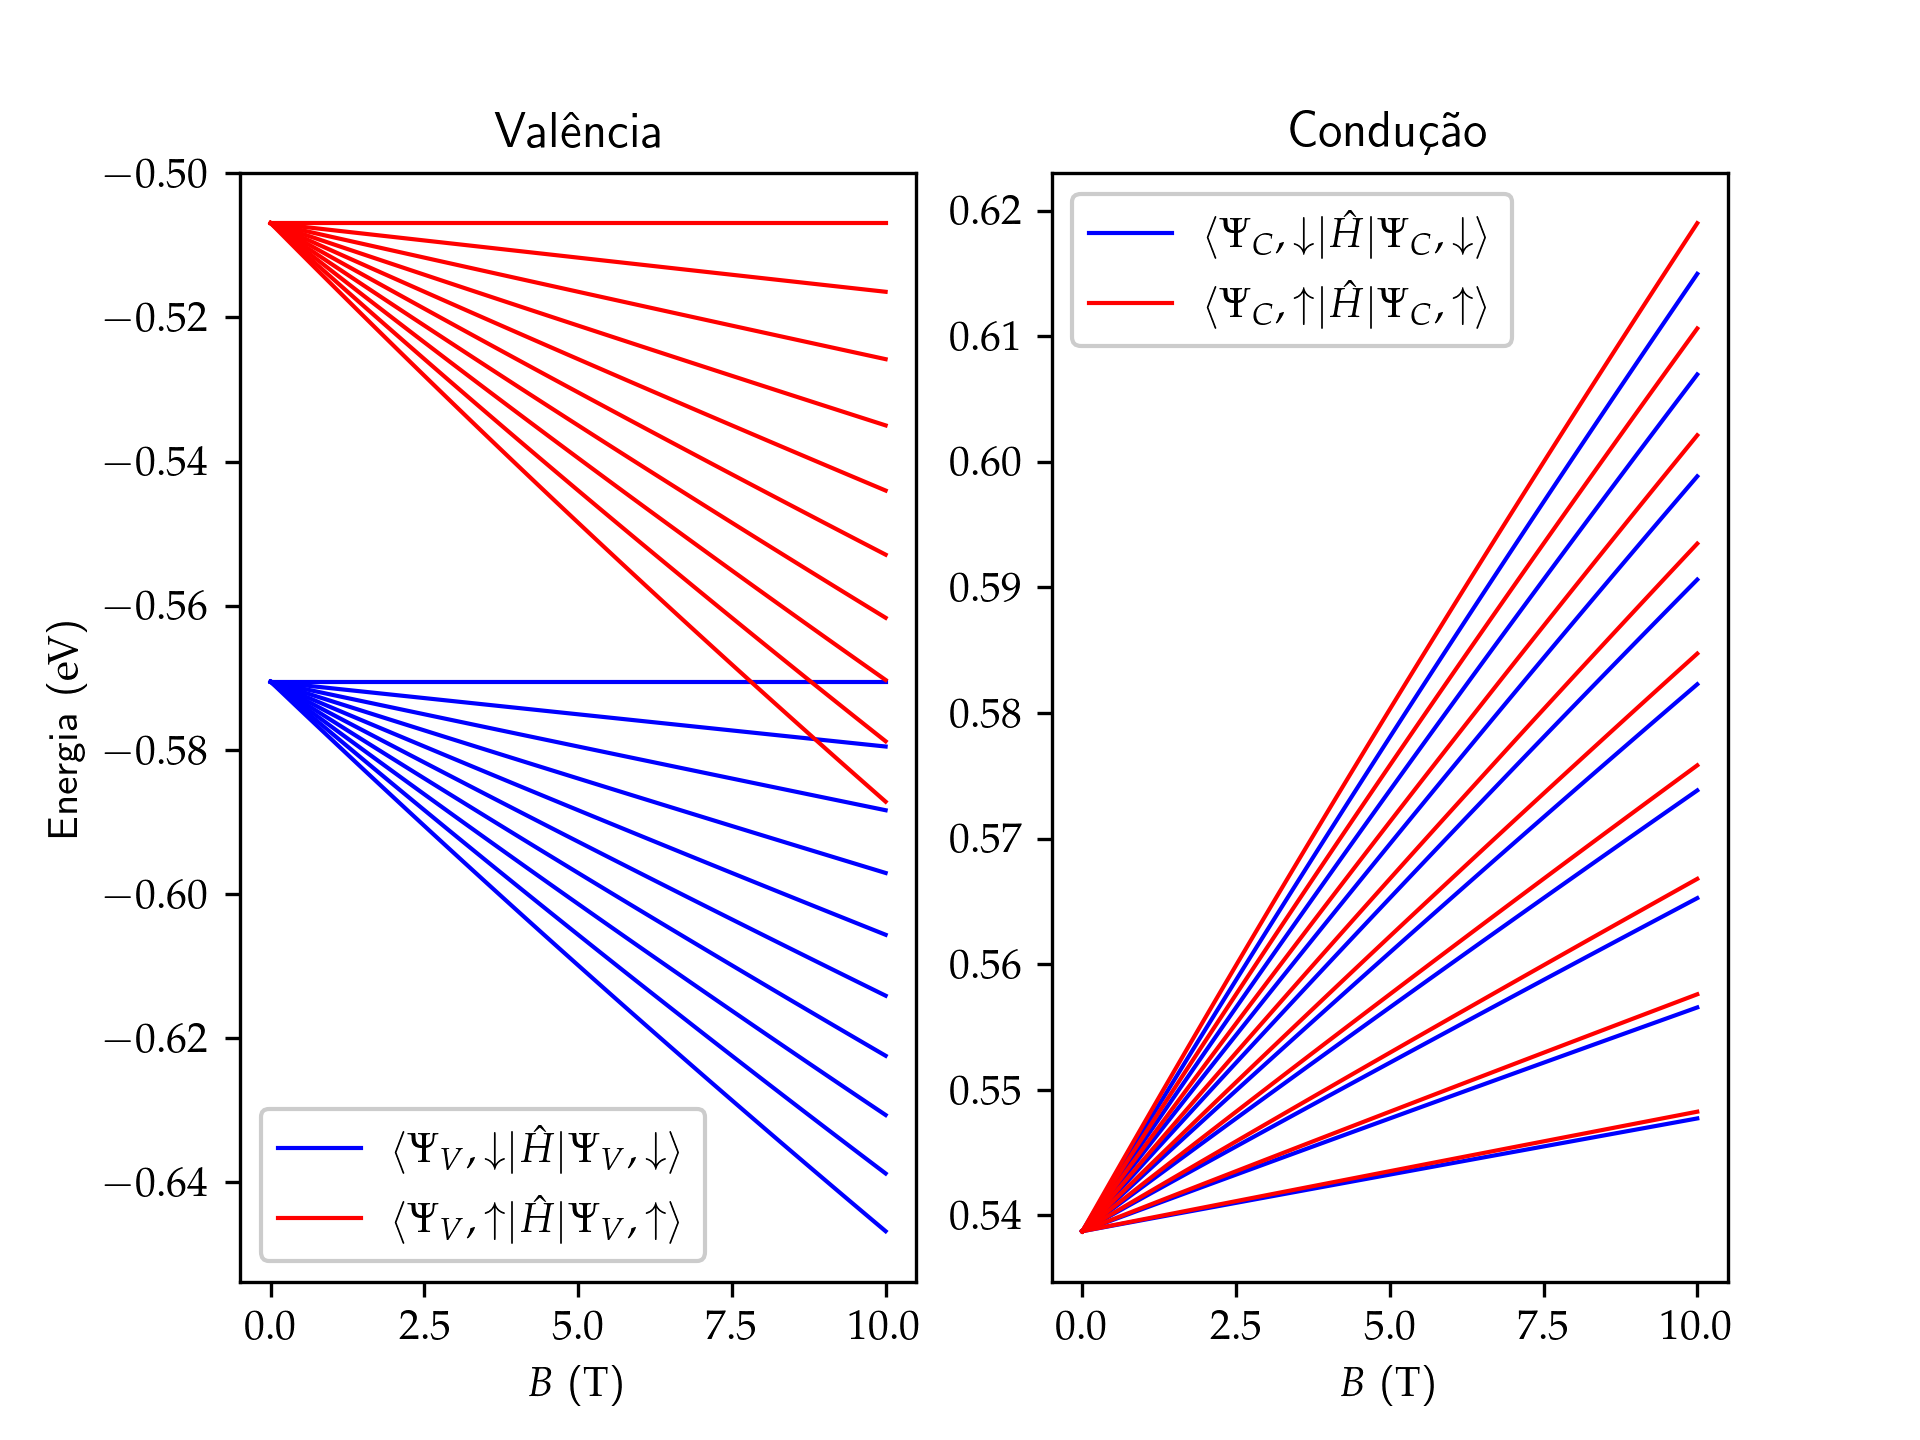
\includegraphics[trim=0 0.28cm 0 0.9cm,clip,width=\textwidth]{imagens/crs2_k_valley_landau_levels.png}
    \caption{}
    \label{fig:crs2_k_valley_landau_levels}
  \end{subfigure}
  \begin{subfigure}{\textwidth}
    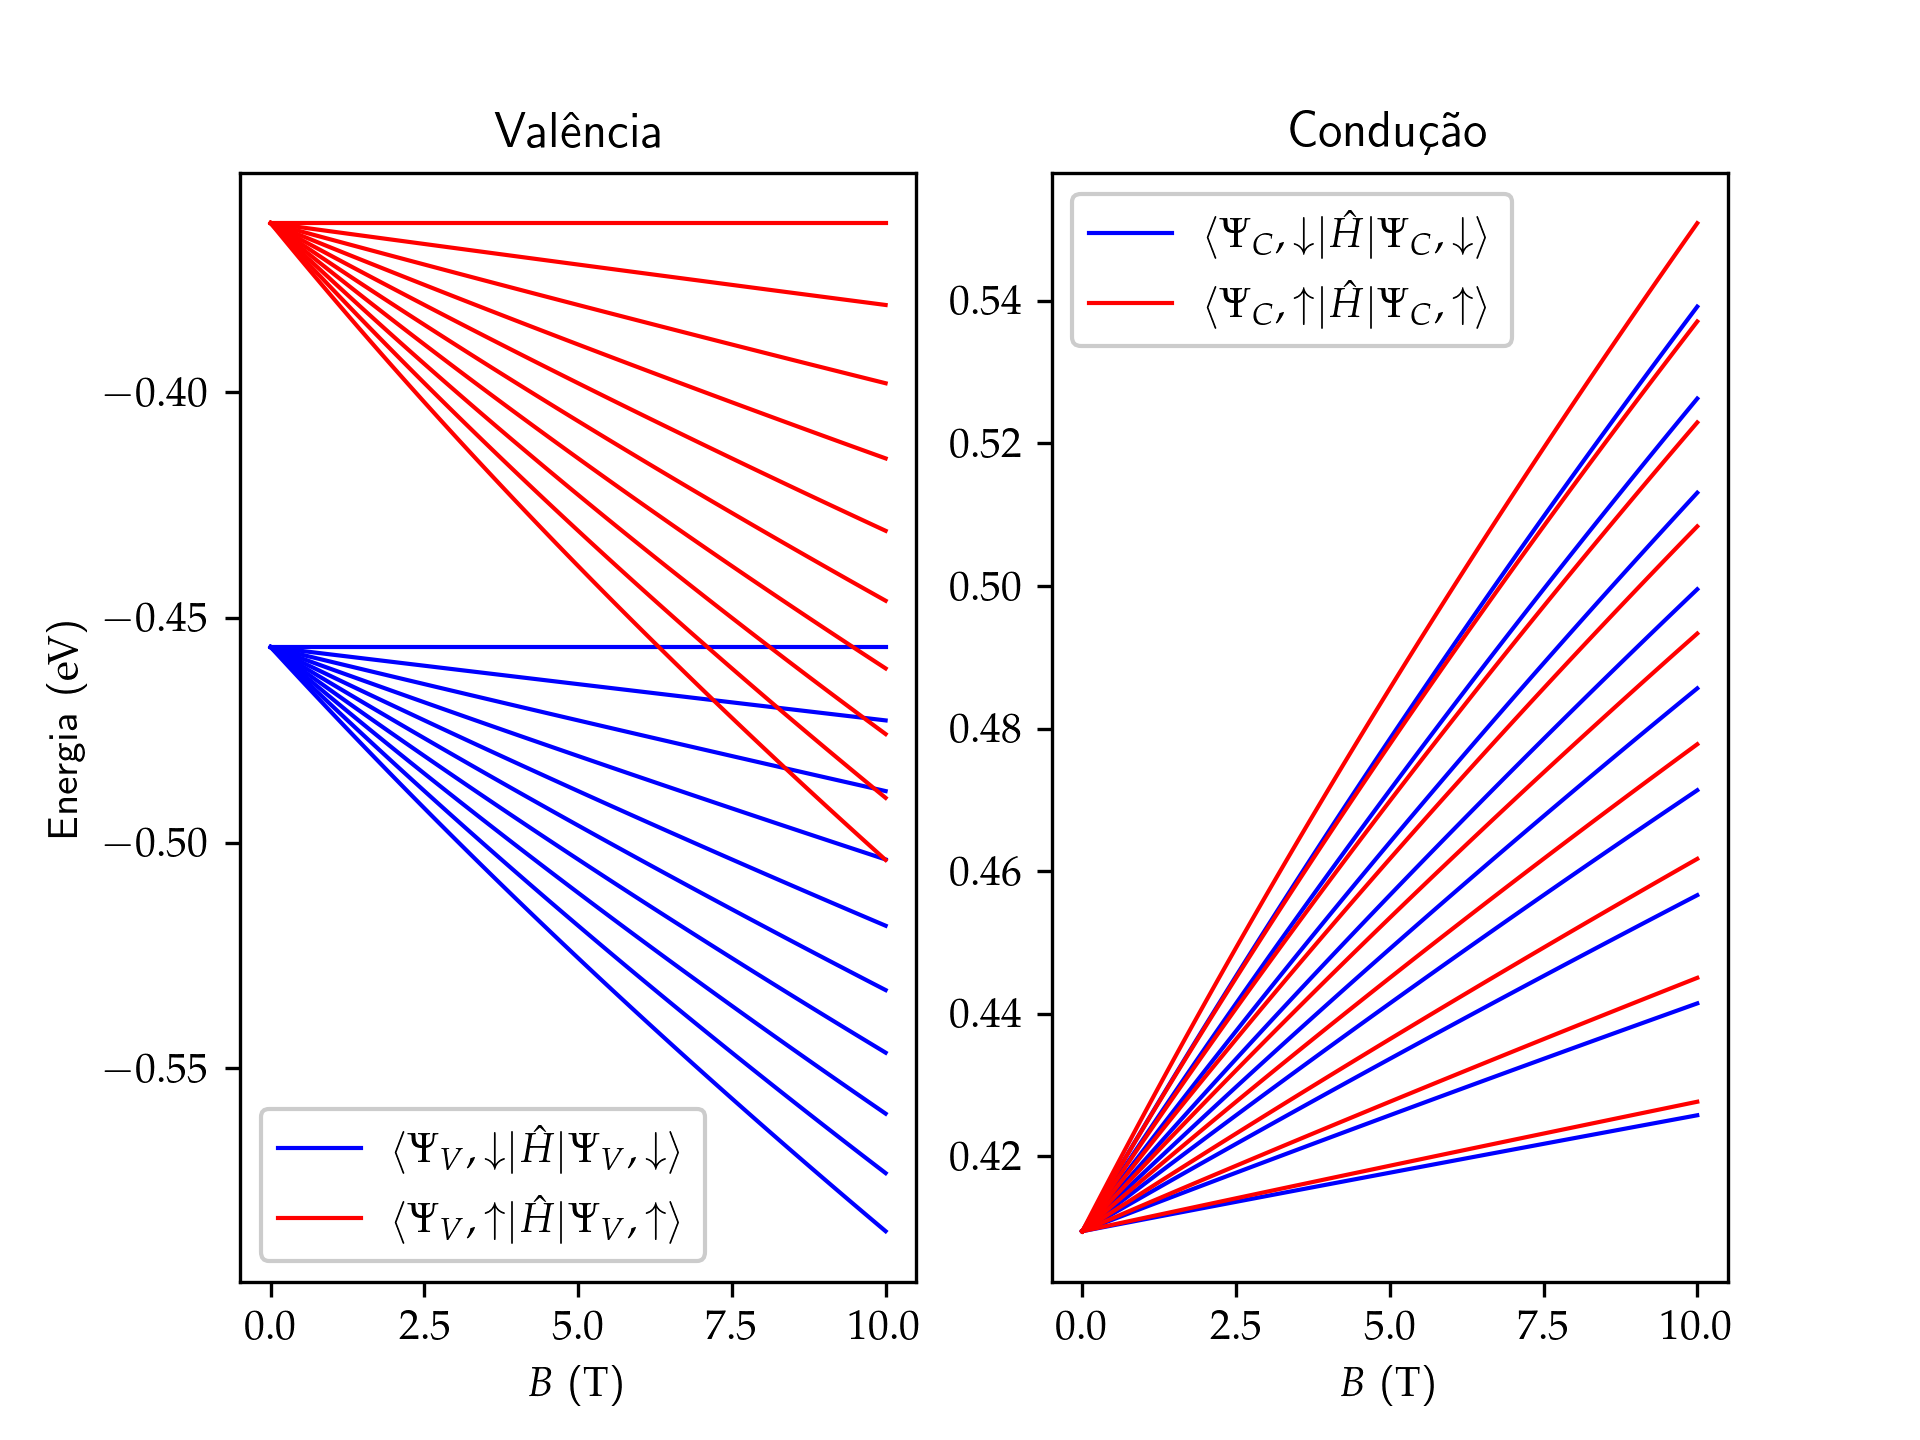
\includegraphics[trim=0 0.28cm 0 0.9cm,clip,width=\textwidth]{imagens/crse2_k_valley_landau_levels.png}
    \caption{}
    \label{fig:crse2_k_valley_landau_levels}
  \end{subfigure}
  \caption{
    Gráficos dos níveis de Landau no vale $K$ para os materiais
    \subref{fig:crs2_k_valley_landau_levels} \ch{CrS2} e
    \subref{fig:crse2_k_valley_landau_levels} \ch{CrSe2} em termos da magnitude
    do campo magnético externo aplicado na direção normal a respectiva
    monocamada.
  }
  \label{fig:k_valley_landau_levels}
\end{figure}

\begin{figure}[p]
  \centering
  \begin{subfigure}{\textwidth}
    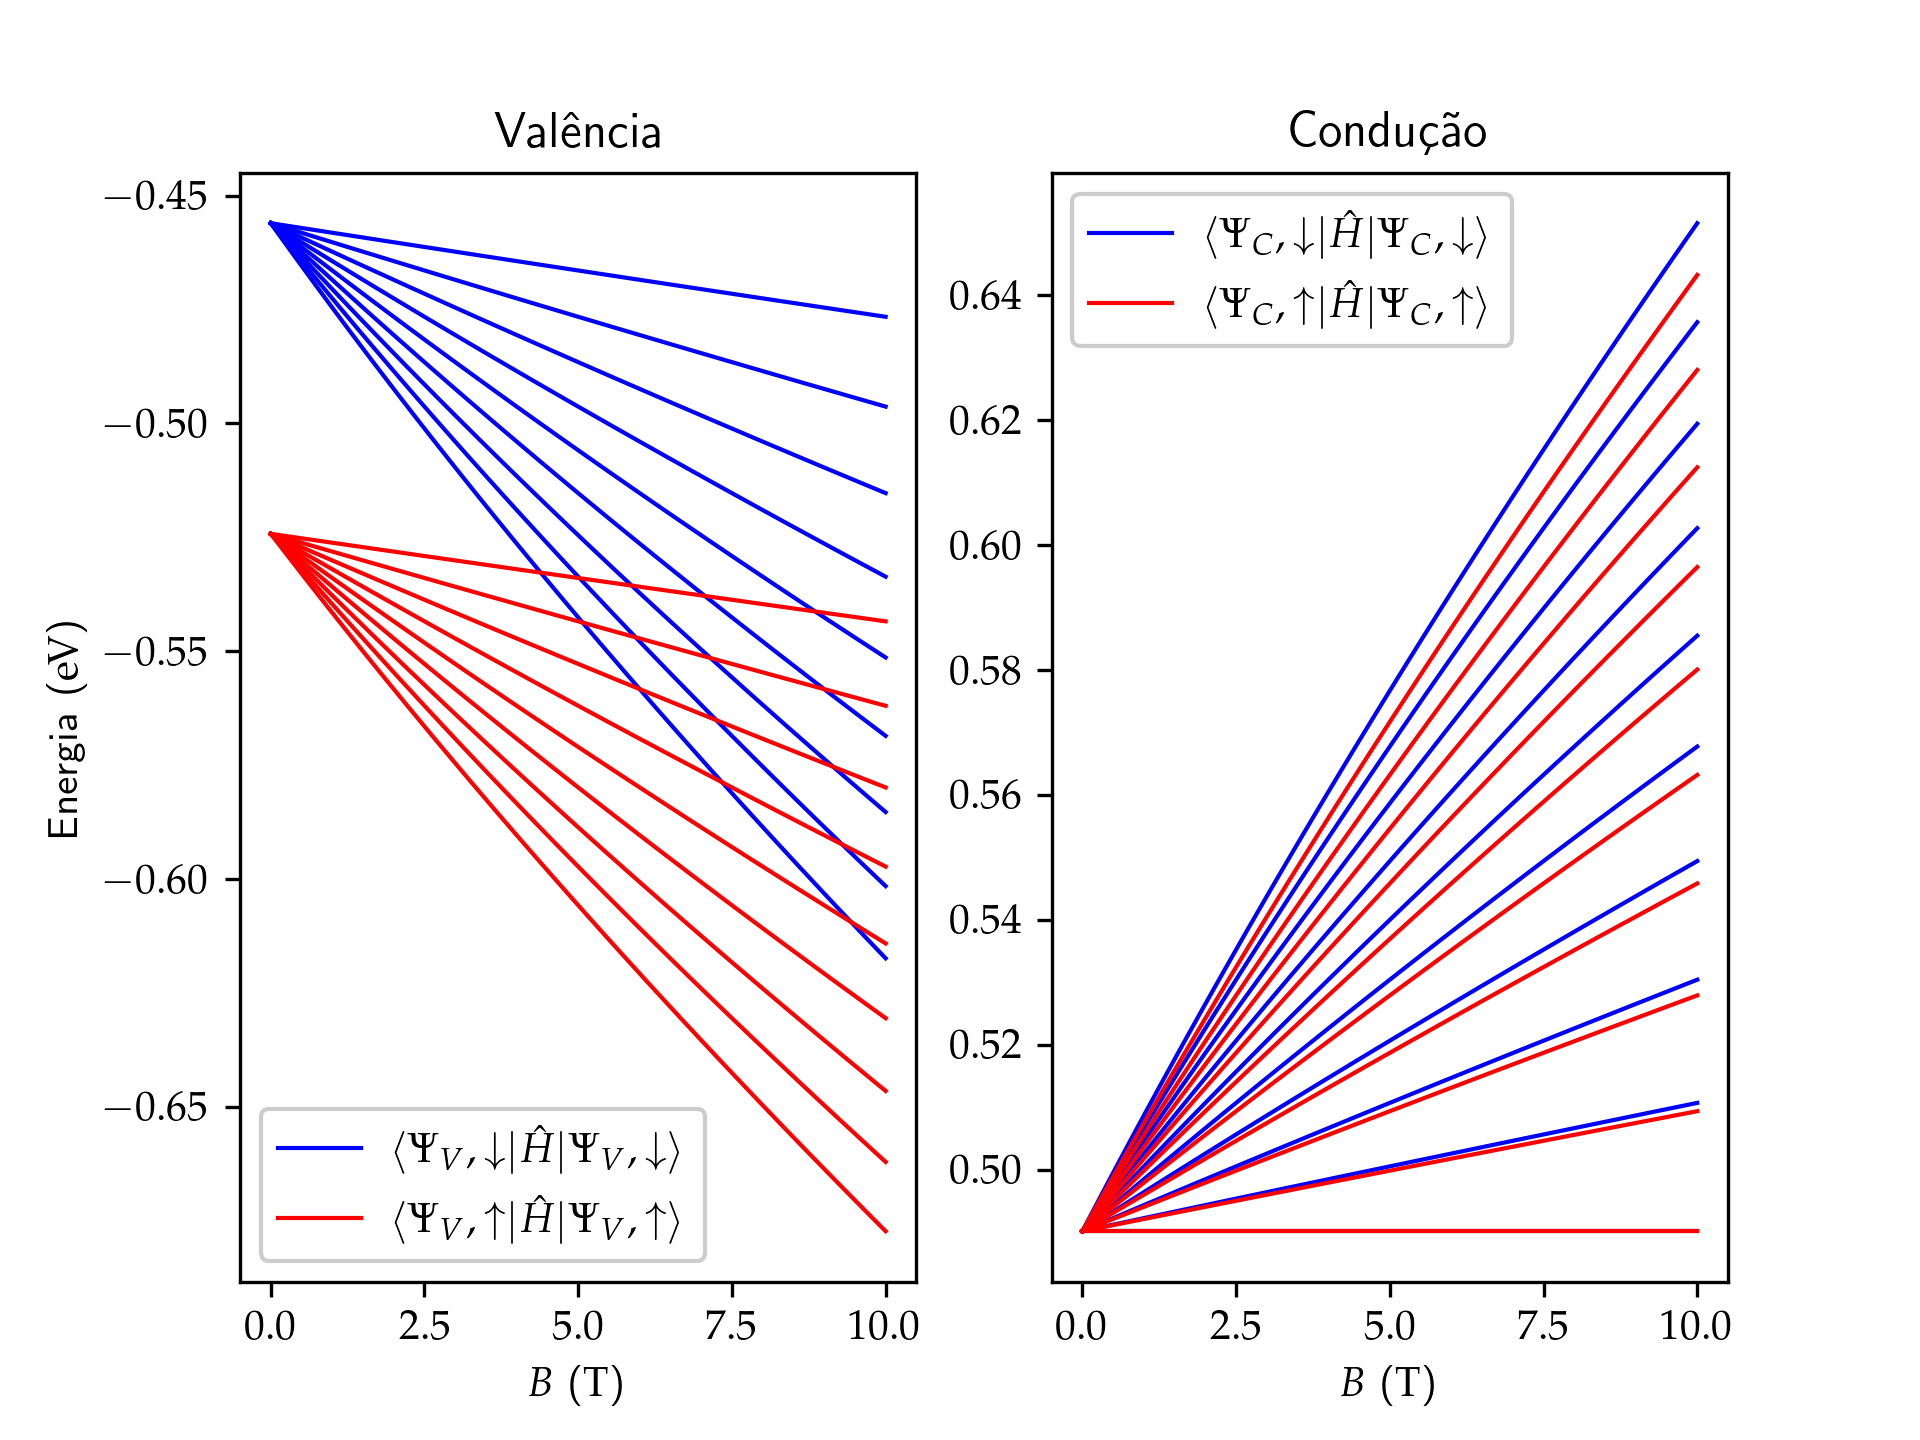
\includegraphics[trim=0 0.28cm 0 0.9cm,clip,width=\textwidth]{imagens/crs2_k_prime_valley_landau_levels.png}
    \caption{}
    \label{fig:crs2_k_prime_valley_landau_levels}
  \end{subfigure}
  \begin{subfigure}{\textwidth}
    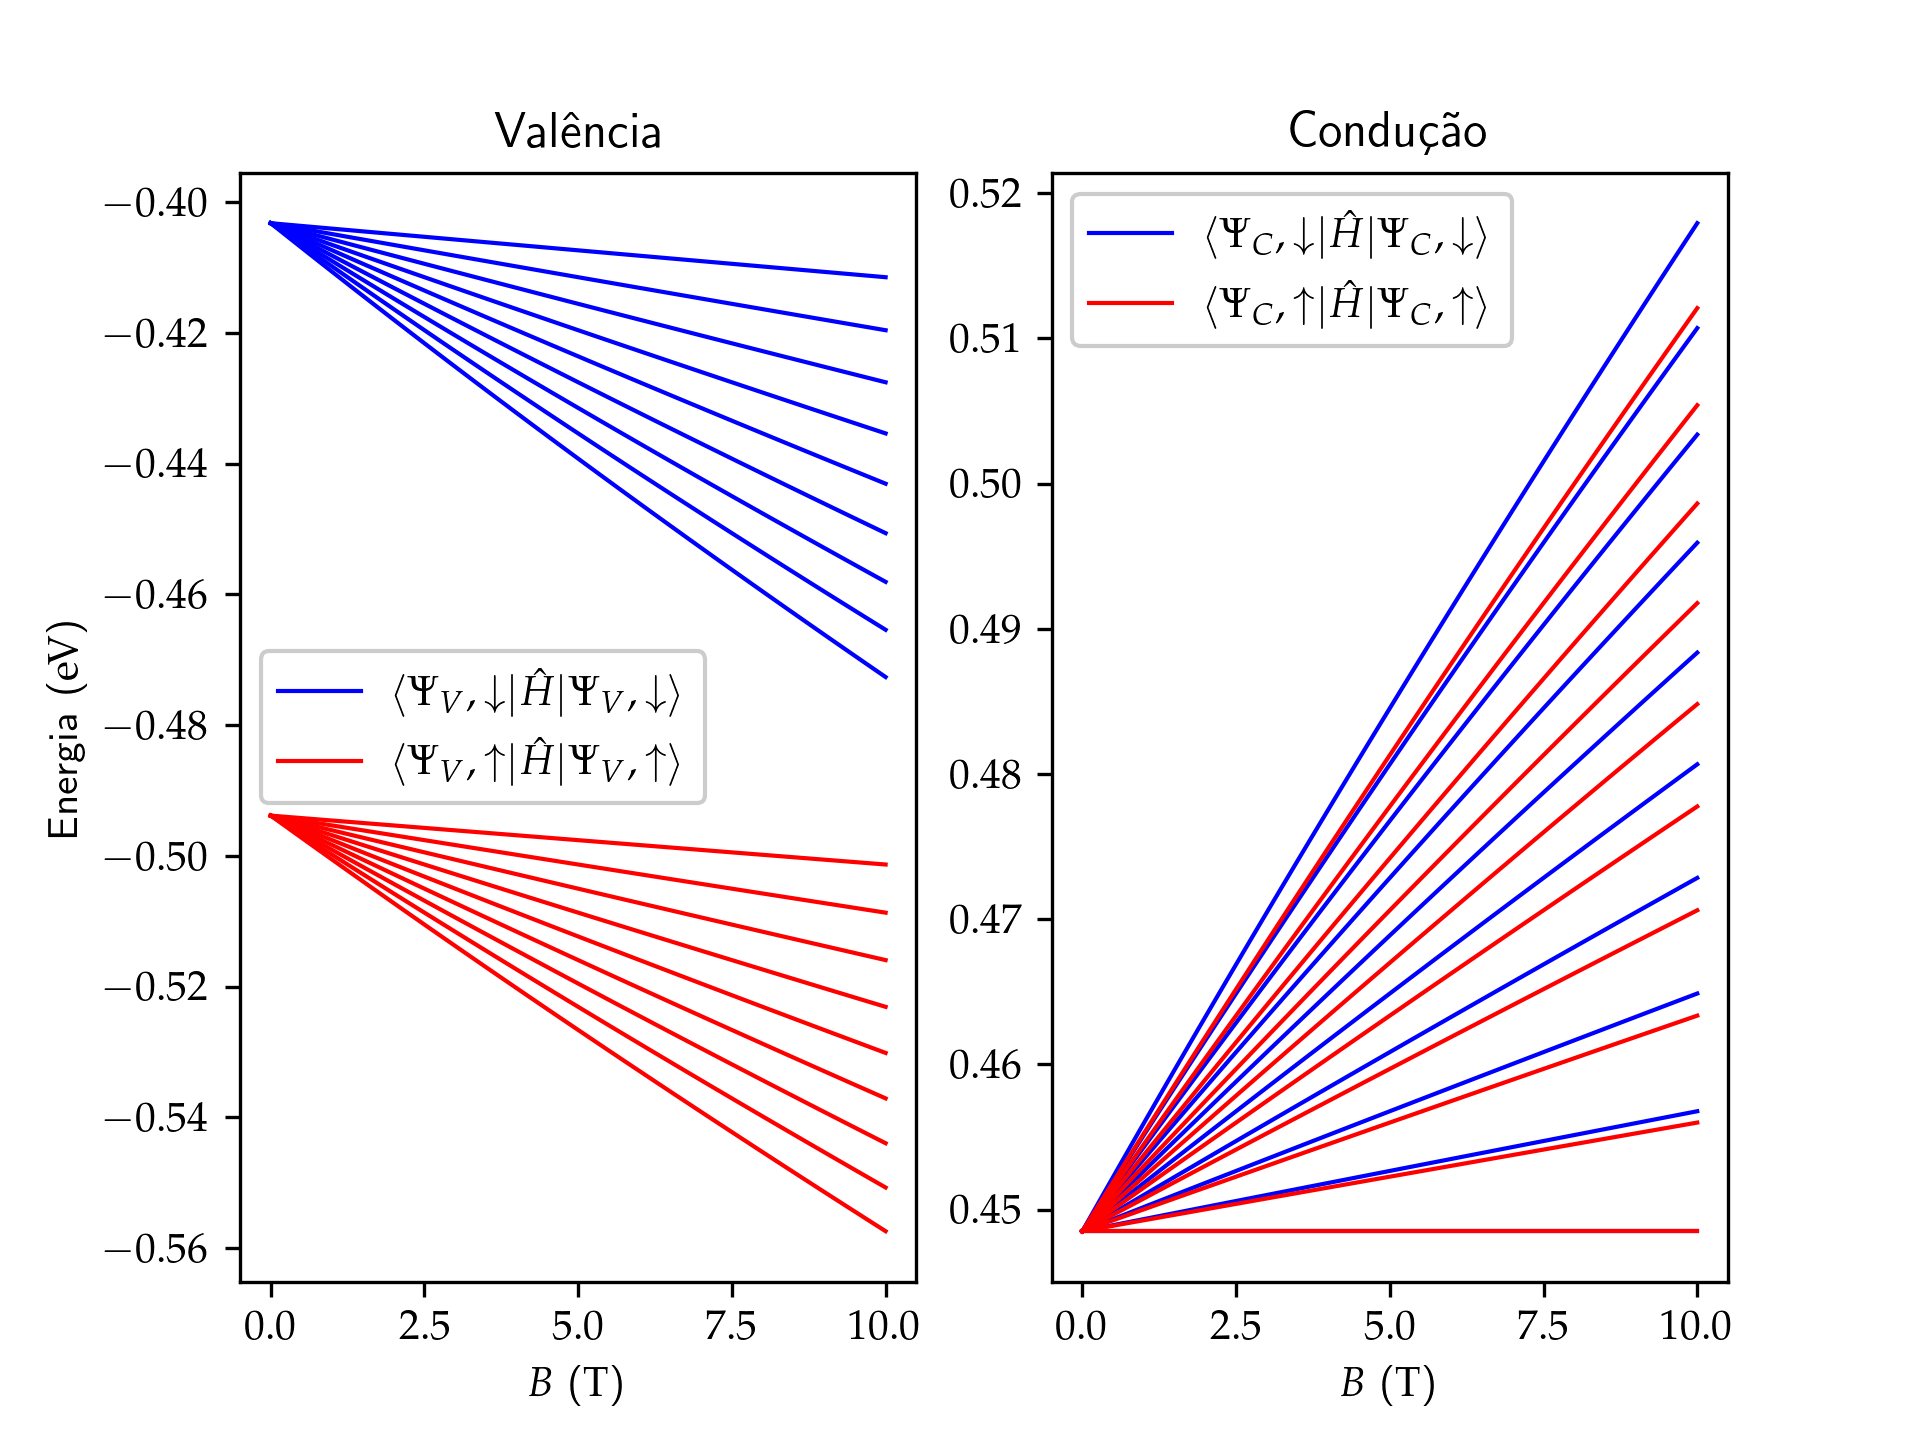
\includegraphics[trim=0 0.28cm 0 0.9cm,clip,width=\textwidth]{imagens/crse2_k_prime_valley_landau_levels.png}
    \caption{}
    \label{fig:crse2_k_prime_valley_landau_levels}
  \end{subfigure}
  \caption{
    Gráficos dos níveis de Landau no vale $K'$ para os materiais
    \subref{fig:crs2_k_prime_valley_landau_levels} \ch{CrS2} e
    \subref{fig:crse2_k_prime_valley_landau_levels} \ch{CrSe2} em termos da
    magnitude do campo magnético externo aplicado na direção normal a respectiva
    monocamada.
  }
  \label{fig:k_prime_valley_landau_levels}
\end{figure}

\begin{figure}[p]
  \centering
  \begin{subfigure}{\textwidth}
    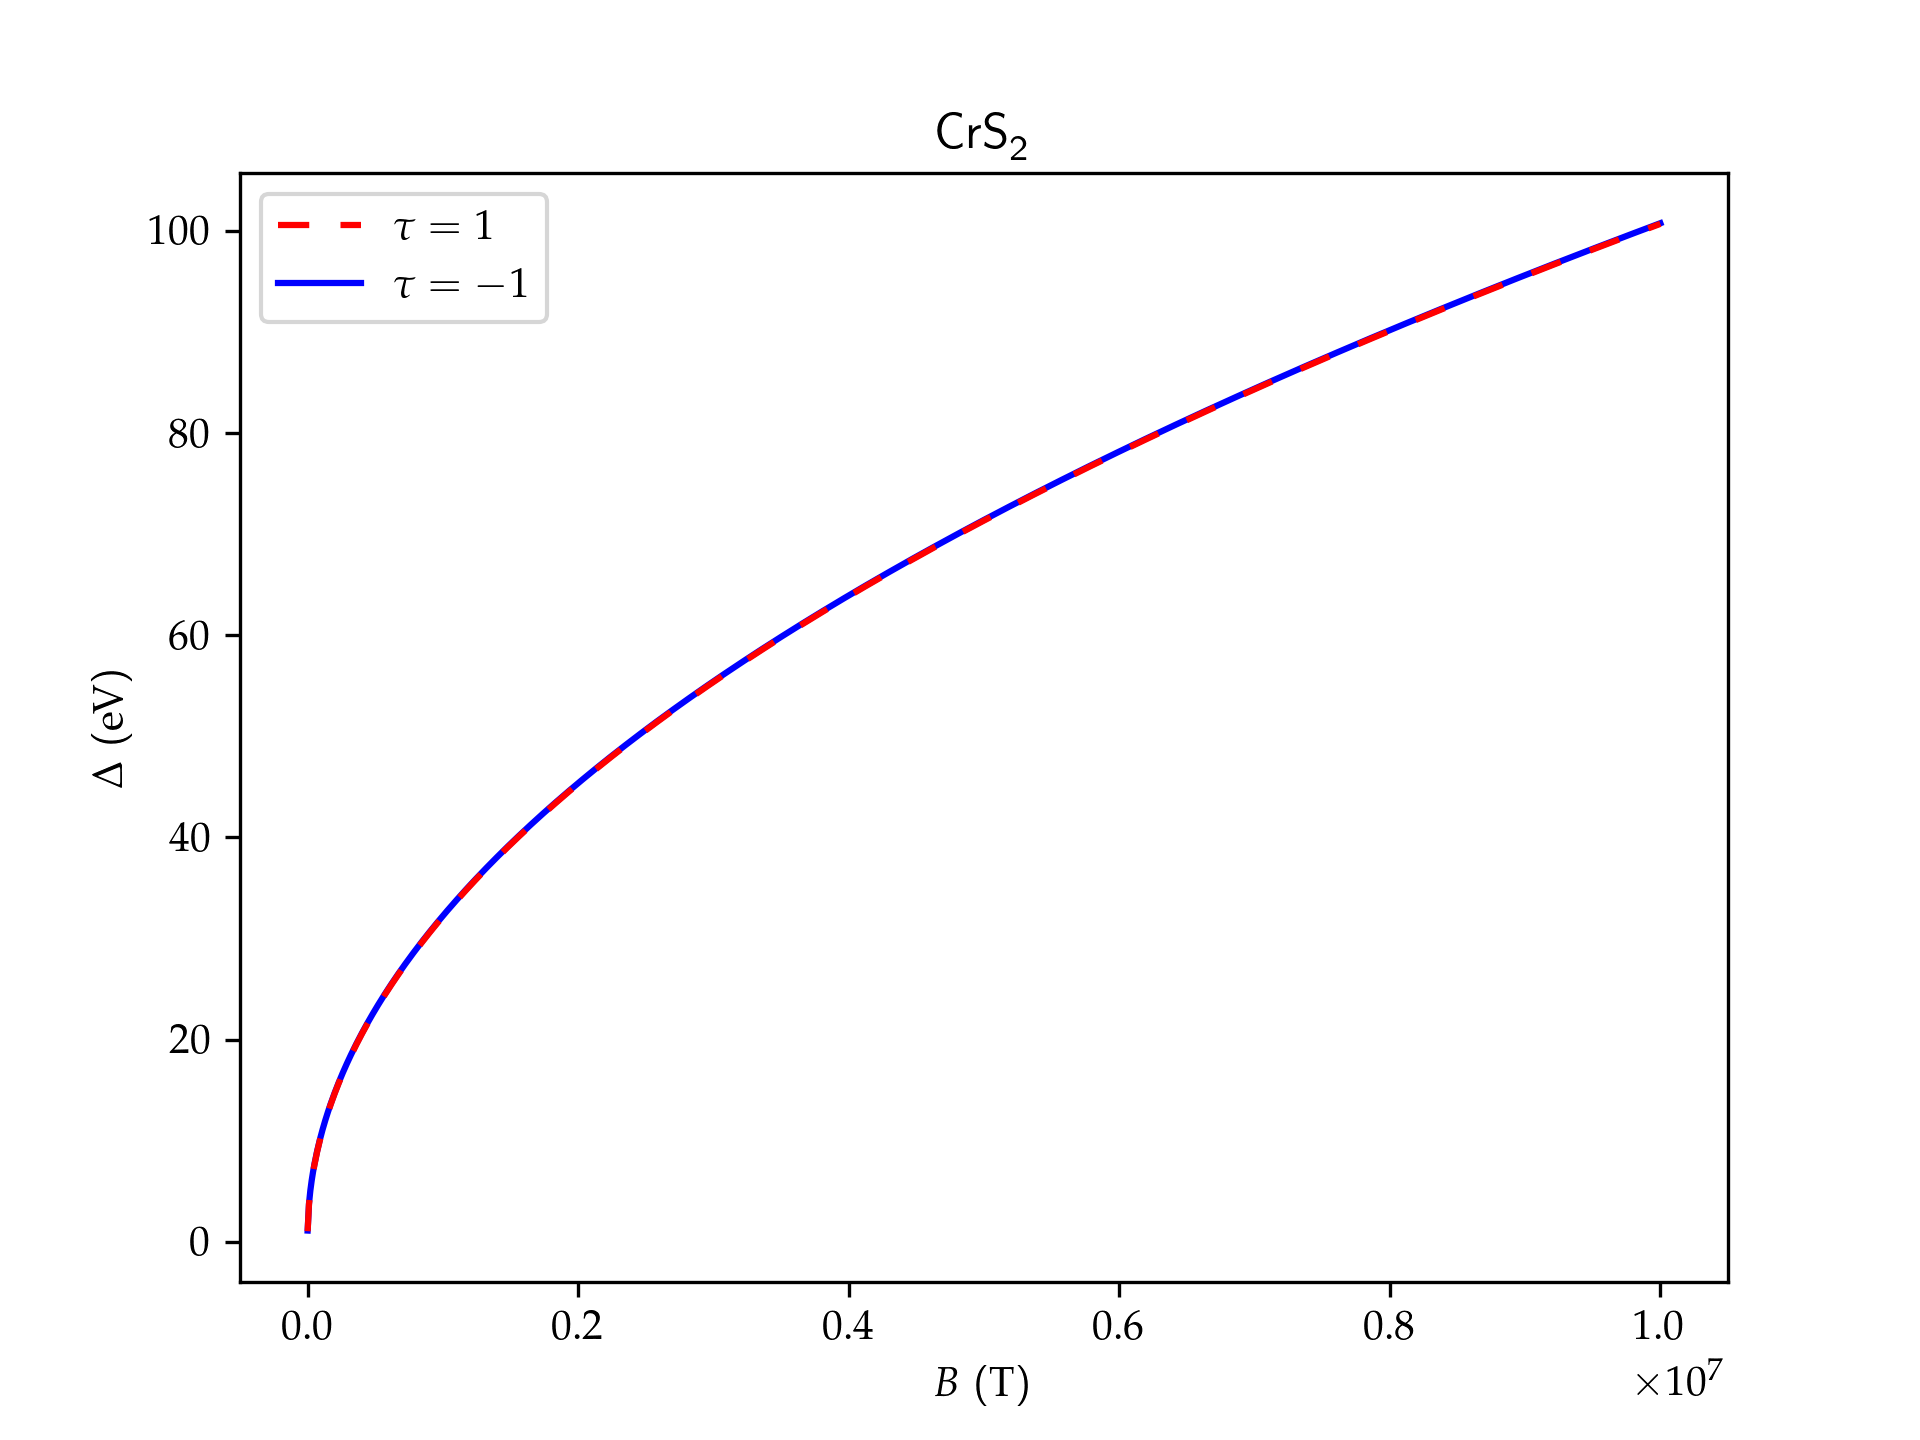
\includegraphics[trim=0 0 0 1.0cm,clip,width=\textwidth]{imagens/crs2_bandgap_field.png}
    \caption{}
    \label{fig:crs2_bandgap_field}
  \end{subfigure}
  \begin{subfigure}{\textwidth}
    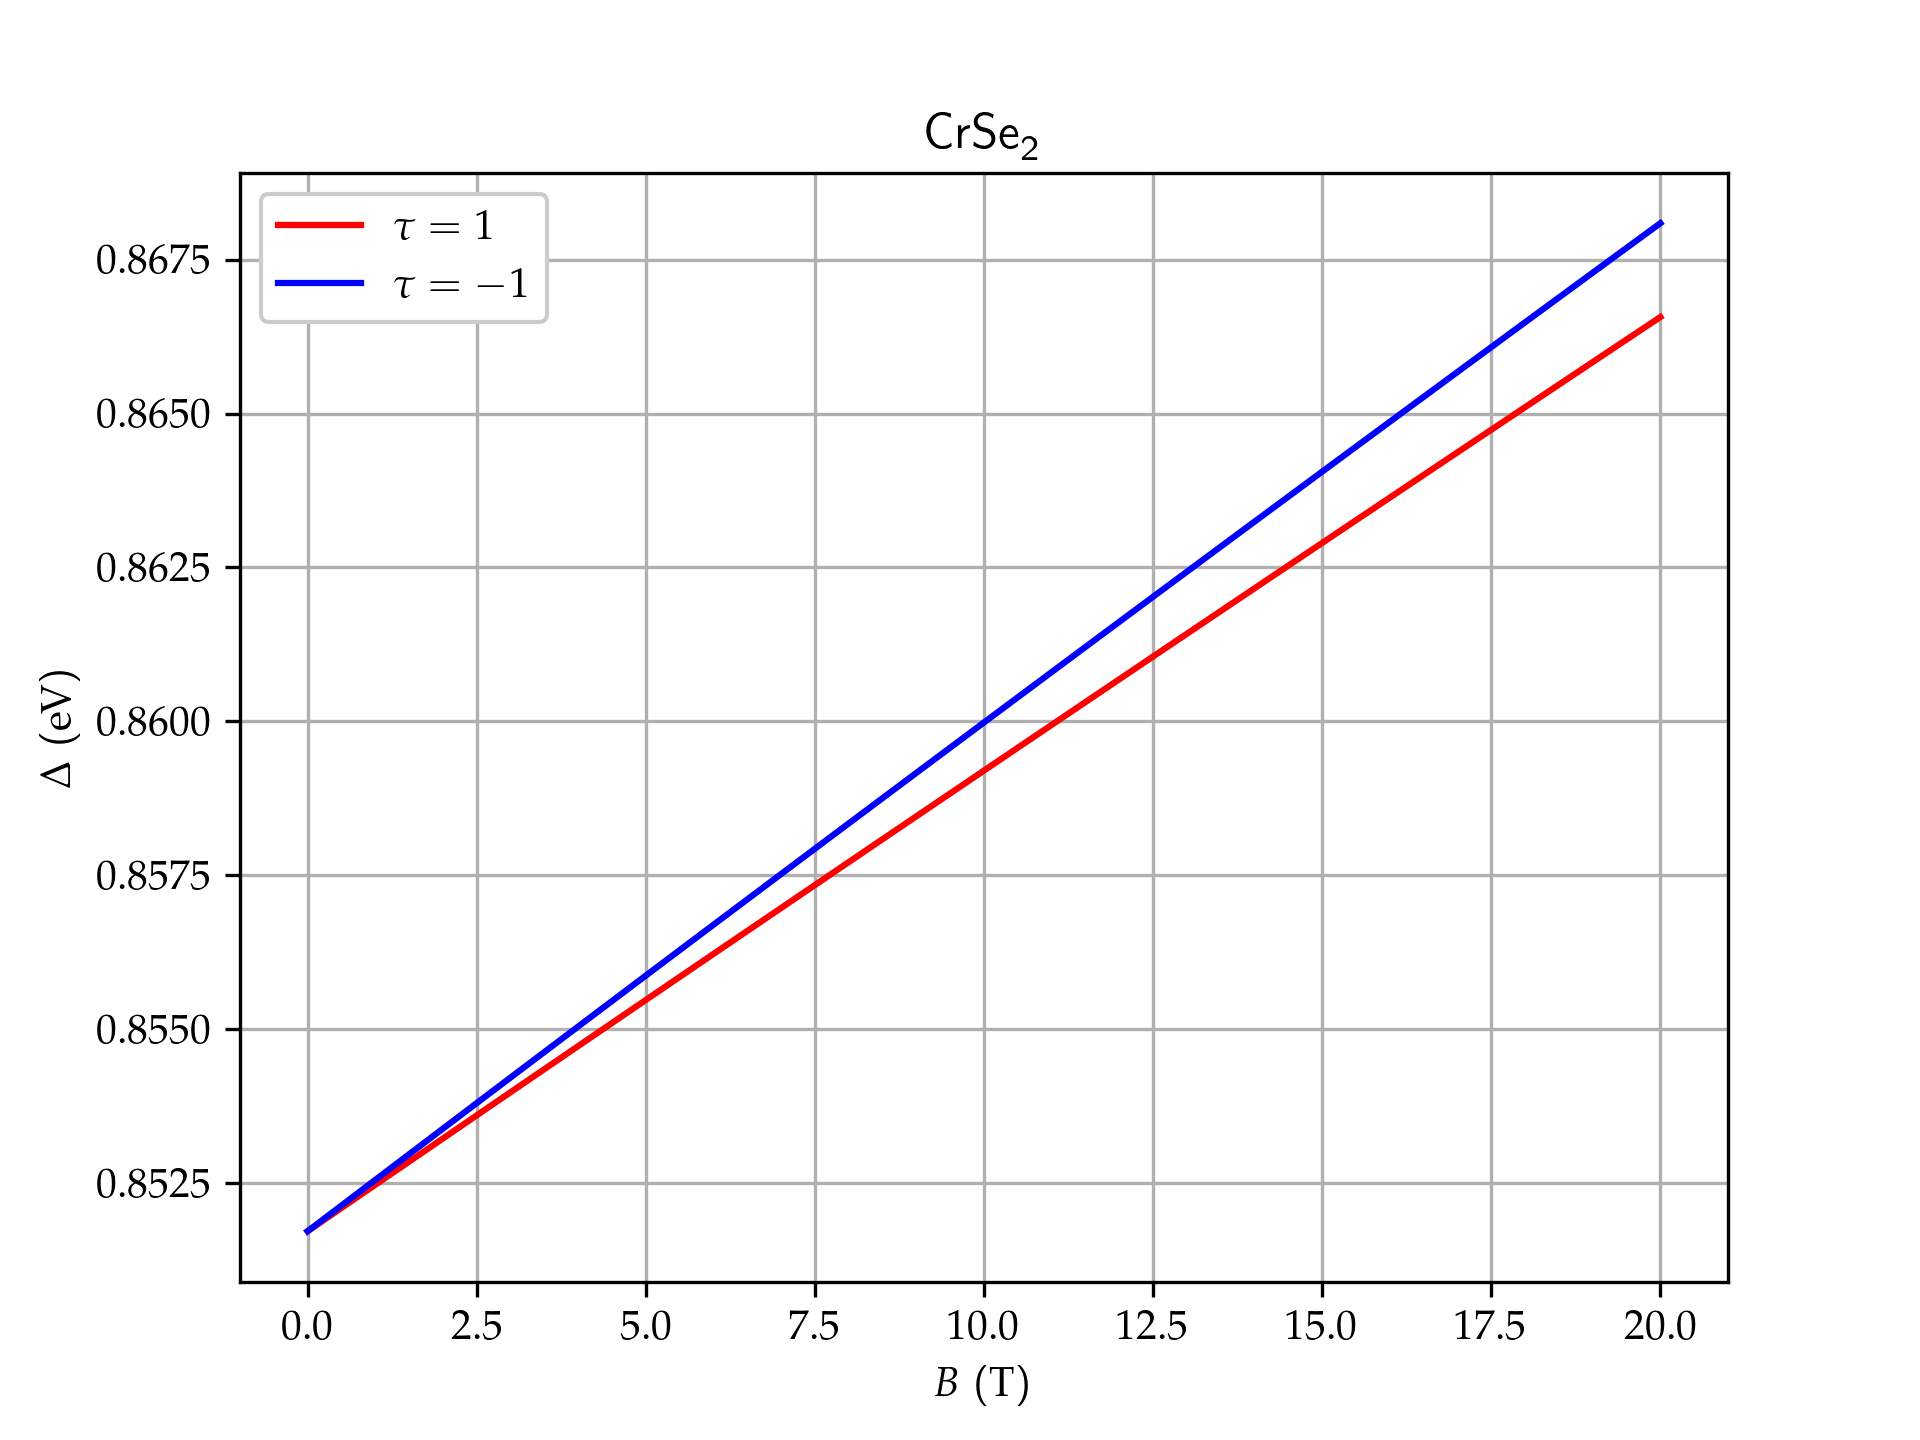
\includegraphics[trim=0 0 0 1.0cm,clip,width=\textwidth]{imagens/crse2_bandgap_field.png}
    \caption{}
    \label{fig:crse2_bandgap_field}
  \end{subfigure}
  \caption{
    Gráficos de $\Delta$ nos vales $K$ e $K'$ para as monocamadas de
    \subref{fig:crs2_bandgap_field} \ch{CrS2} e \subref{fig:crse2_bandgap_field}
    \ch{CrSe2} em termos da magnitude do campo magnético externo.
  }
  \label{fig:bandgap_field}
\end{figure}

\section{Testes de Performance}

Em testes de tempo de execução o algoritmo desenvolvido escalou bem, sendo sua
complexidade temporal $\mathcal{O}(n)$ para o tamanho de população, e
$\mathcal{O}(g)$ para número de gerações decorridas. 

Nas figuras exibidas na
Seção \ref{sec_test_functions}, o tempo médio decorrido na evolução das
populações de 1000 indivíduos foi de 15 segundos\footnote{
  Tempo obtido usando uma máquina com processador Intel® Core™ i7-8550U com 8
  processadores lógicos com frequência base de operação de 1,8GHz e frequência
  máxima de 4GHz. É importante frisar aqui as evoluções das 8 populações ocorreram
  em 8 processos concorrentes. Assim, é possível que, para uma única população, os
  tempos de execução sejam ligeiramente menores, abdicando da escala da população. 
} enquanto que o tamanho da população necessário
para que o processo tomasse mais de uma hora foi superior a $n = 10^5$, para o
mesmo número de gerações.

Já para os ajustes feitos na Seção \ref{sec_resultados_tmdcs}, o tempo médio
demandado para a evolução dos 16000 indivíduos pelas 200 gerações foi cerca de
15 minutos para o ajuste de 1ª ordem e 25 minutos para o ajuste de 3ª ordem
\footnote{
  Tempo obtido usando uma máquina com processador  Intel® Xeon® E5-2650 v2 com 16
  processadores lógicos com frequência base de operação de 2,6GHz e frequência
  máxima de 3,4GHz. Novamente, as iterações de cada uma das 16 populações
  ocorreram em 16 processos concorrentes. As mesmas condições foram usadas
  para a otimização via \textit{Dual Annealing}.
}. Em contrapartida, os ajustes feitos pelo método alternativo 
\textit{Dual Annealing} tomaram em média um tempo de 2 minutos para a expansão de 1ª ordem e
10 minutos para os cálculos de 3ª ordem.

O fato desse método também ser implementado em Python via NumPy\footnote{
  Código-fonte disponível em \url{https://github.com/scipy/scipy/blob/main/scipy/optimize/_dual_annealing.py}.
} sugere que melhorias podem ser feitas na implementação realizada para a confecção
deste trabalho, de forma a melhorar o desempenho. Isso deve ser feito reformulando
os códigos-fonte em questão de forma a abusar ao máximo das estruturas de dados e
funções da biblioteca NumPy, uma vez que estes agregam mais performance.

Todavia, esta diferença no tempo de execução de ambos os métodos não faz do
algoritmo proposto no Capítulo \ref{cap_metodologia} uma estratégia ineficaz, já
que foram atingidos resultados favoráveis. Resultados com valores ainda menores
para $f$ podem ser atingidos com o uso de mais iterações e de outras combinações
de valores para $p_2$, $p_3$, $e_1$, $e_2$, $e_3$ e $h$, po que não foi explorado
na obtenção dos resultados da seção anterior.
\chapter{Conclusão}\label{cap_conclusao}

Texto da conclusão. 


\chapter{Cronograma}\label{cap_cronograma}

Neste capítulo são apresentadas as atividades realizadas até o momento da confecção deste
trabalho, bem como as perspectivas para o próximo período.

\begin{itemize}
  \item Período 2021/02\trav Nesse período foi feita a leitura da bibliografia citada neste
        texto, e então foi implementada a primeira versão do algoritmo. 
        Posteriormente, foi feita uma série de testes com diferentes funções, dentre as quais
        estão as citadas nesse trabalho. Finalmente, foi confeccionado este texto.
  \item Período 2022/01\trav No período subsequente, planeja-se escolher um problema físico
        que envolva a otimização de funções, realizar uma consulta sobre referências bibliográficas
        relacionadas, fazer a leitura dos dos textos encontrados e aplicar o programa na solução
        do problema. Por fim, o Trabalho de Conclusão de Curso será elaborado acerca dos
        resultados obtidos e a defesa dessa tese será apresentada.
\end{itemize}


% ---
% Finaliza a parte no bookmark do PDF
% para que se inicie o bookmark na raiz
% e adiciona espaço de parte no Sumário
% ---
\phantompart

% ---
% Conclusão (outro exemplo de capítulo sem numeração e presente no sumário)
% ---
% \include{conclusao.tex}
% ---

% ---
% Elementos Pós Textuais
% ---
\postextual

% ---
% Referências bibliográficas
% ---
\bibliography{bibliografia.bib}

\end{document}
